% !TEX program = lualatex
\documentclass[11pt,twoside]{thesisA4}
\usepackage{rotating}
\usepackage{csquotes}
\usepackage[type={CC},modifier={by-sa},version={4.0}]{doclicense}
\usepackage{tikz}
\usetikzlibrary{shapes.geometric, arrows.meta, positioning}
\makeatletter\def\abx@dot{.}\makeatother
\addbibresource{references.bib} % duplicate for VS Code intellisense (also in thesis.cls)

% lualatex -interaction=nonstopmode main.tex
% makeglossaries main
% biber main
% lualatex -interaction=nonstopmode main.tex
% lualatex -interaction=nonstopmode main.tex

\loadglsentries{acronyms}
\loadglsentries{terms}

\begin{document}

\blankpage



\makefrontcover

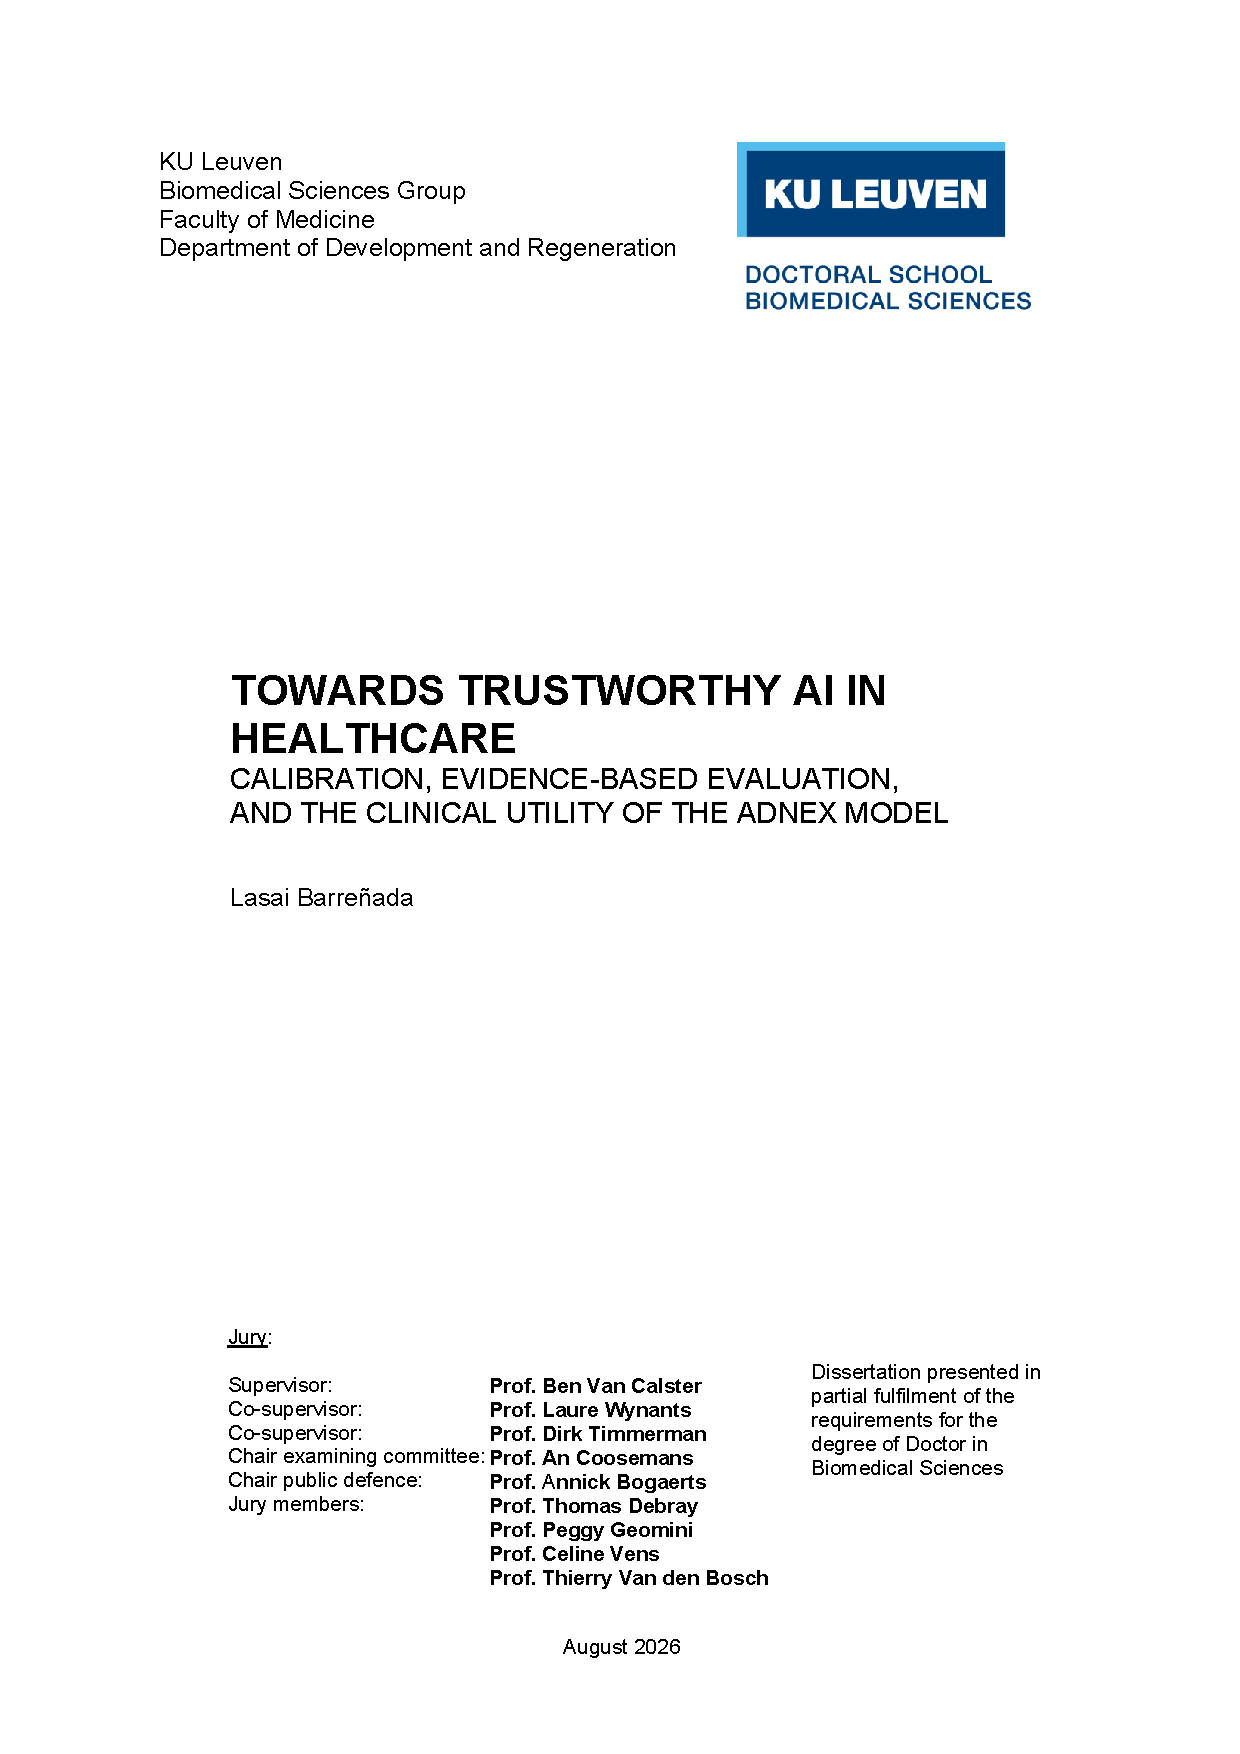
\includepdf[pages=-]{title_page/title_page.pdf}

\makecopyrightpage{Lasai Barreñada}{Herestraat 49, 3000 Leuven (Belgium)}

\newpage
\thispagestyle{empty}

\vspace*{\fill}
\begin{center}
	\begin{minipage}{0.85\textwidth}
		\itshape\large
		We shall try not to use statistics as a drunken man uses lamp-posts,
		for support rather than for illumination.

		\par\vspace{1em}
		\raggedleft\normalfont
		-- Andrew Lang, Scottish poet and novelist
	\end{minipage}
\end{center}
\vspace*{\fill}

\blankpage
\newpage

\pagenumbering{roman}

% \chapter*{Acknowledgments}
\addcontentsline{toc}{chapter}{Acknowledgments}

Hello everyone,

This is me expressing my heartfelt gratitude to all those who have supported me throughout my PhD journey.

First and foremost, I would like to thank my supervisor, Prof. Dr. Jane Smith, for her unwavering support, guidance, and encouragement. Her expertise and insights have been invaluable in shaping my research and academic growth.
I am also deeply grateful to my colleagues and friends at the Research Lab for creating a collaborative and stimulating environment. Special thanks to John Doe and Emily Davis for their assistance with experiments and data analysis.
Finally, I would like to extend my sincere thanks to my family for their love and support throughout this journey. Their belief in me has been a constant source of motivation.
End of acknowledgments.



{\raggedleft
holahoal \\ % tighten space here
Lasai Barreñada \\
August 2026 \\
}
\chapter*{Abstract}
\addcontentsline{toc}{chapter}{Abstract}
The ADNEX model, introduced in 2014, has demonstrated good diagnostic ability for five ovarian tumor types: benign, borderline, stage I invasive, stage II-IV invasive, and secondary metastasis. However, ADNEX should be further improved based on previous findings. First, despite excellent overall performance, we should understand and reduce observed differences between centers. Second, ADNEX was developed on patients selected for surgery, and should be adapted to work for all patients with a newly detected tumor. Third, we need to understand whether ADNEX works less well when used by clinicians with limited experience. Fourth, we should compare different statistical algorithms for developing the model. Finally, ADNEX is the fruitful result of a combination of clinical and statistical research. Therefore, we need to continue the statistical research on prediction modeling. In particular, we are interested in development and validation of machine learning models in the presence of multicenter (i.e. clustered) data, and in variable selection methods based criteria for clinical utility rather than for statistical performance.
\chapter*{Samenvatting}
\addcontentsline{toc}{chapter}{Samenvatting}
Klinische voorspellingsmodellen kunnen evidence-based klinische besluitvorming ondersteunen door het ziekterisico van een patiënt in te schatten. Voor een veilig en effectief gebruik ervan is echter meer nodig dan alleen een goede gemiddelde onderscheidingskracht: de voorspelde waarschijnlijkheden moeten nauwkeurig (d.w.z. gekalibreerd) en klinisch bruikbaar zijn, en voldoende robuust om rekening te houden met verschillen tussen centra, meetprocedures en patiëntenpopulaties.

Dit proefschrift combineert toegepast en methodologisch onderzoek om de besluitvorming voor vrouwen met adnexale massa's te verbeteren, met een focus op het Assessment of Different NEoplasias in the adneXa (\gls{ADNEX})-model voor de diagnose van eierstokkanker.

Ten eerste heb ik het bewijsmateriaal uit externe validatiestudies voor \gls{ADNEX} samengevat. Een systematische review en meta-analyse van 47 studies met in totaal meer dan 17.000 tumoren bevestigde een sterke onderscheidende waarde (AUC 0,93 voor goedaardige versus kwaadaardige gezwellen), maar toonde ook aan dat de kwaliteit van de methodologische rapportage te wensen overlaat: 91\% van de validaties vertoonde een hoog risico op vertekening en de kalibratie werd zelden beoordeeld. Ten tweede presteerde \gls{ADNEX} in een rechtstreekse systematische review en meta-analyse van 11 studies (8271 tumoren) consequent beter dan de Risk of Malignancy Index (\gls{RMI}) wat betreft discriminatievermogen en klinisch nut; bij een drempelwaarde van 10\% voor het risico op maligniteit was de kans dat de test bruikbaar zou zijn in een hypothetisch nieuw centrum 96\% voor \gls{ADNEX} en 15\% voor \gls{RMI}. Ten derde heb ik \gls{ADNEX} geüpdatet naar \emph{ADNEX2} met behulp van prospectieve gegevens uit meerdere centra, waaronder ook conservatief behandelde patiënten, waardoor het model beter kan worden ingezet in een tweestappenstrategie die begint met de goedaardige, eenvoudige descriptoren. 


Het methodologische deel van dit proefschrift behandelt bredere uitdagingen op het gebied van waarschijnlijkheidsschatting en modelevaluatie. Ik heb onderzocht waarom random forest-modellen met uitstekende trainingsprestaties toch onstabiele of misleidende waarschijnlijkheden kunnen opleveren, en heb aangetoond hoe random forests lokale waarschijnlijkheidspieken kunnen leren waarvoor gangbare standaardinstellingen (volledig volgroeide bomen) contraproductief kunnen zijn wanneer het doel een goed gekalibreerde risicoschatting is. Vervolgens heb ik geclusterde kalibratiemethoden ontwikkeld die expliciet rekening houden met een multicenterstructuur, waardoor kalibratie niet alleen op basis van het gemiddelde kan worden samengevat, maar ook met voorspellingsintervallen die de verwachte variabiliteit tussen centra kwantificeren. Ten slotte stelde ik een raamwerk voor onzekerheid in individuele risicoschattingen voor en illustreerde ik empirisch dat, zelfs met grote trainingssteekproeven, de onzekerheid ongerustmakend groot is. Dit ondersteunt het idee dat modellen altijd met de nodige voorzichtigheid moeten worden geïnterpreteerd en dat beslissingen moeten worden genomen door deskundige artsen die de risicoschatting in de juiste context kunnen plaatsen. Tot slot introduceer ik een algoritme voor variabele selectie dat het klinisch nut optimaliseert, waarbij wordt gewaarborgd dat de geselecteerde voorspellende variabelen klinisch relevant zijn, rekening houdend met de kosten van het meten ervan.

Dit proefschrift levert een bijdrage aan het vakgebied van klinische voorspellingsmodellen door nieuw bewijs te leveren over de prestaties van \gls{ADNEX} en door de ontwikkeling van \emph{ADNEX2}, en door nieuwe methoden te ontwikkelen voor het opstellen en valideren van voorspellingsmodellen die in een breed scala aan klinische contexten kunnen worden toegepast. De bevindingen hebben belangrijke implicaties voor de ontwikkeling en validatie van klinische voorspellingsmodellen, zodat deze uitgroeien tot betrouwbare en bruikbare hulpmiddelen voor de klinische besluitvorming.

\tableofcontents

\addcontentsline{toc}{chapter}{Glossary}
\renewcommand*{\glossarypreamble}{\noindent\textit{Terms shown in bold at first mention are defined in this glossary. Definitions in this glossary are provided in the context of clinical prediction modelling and are tailored to the scope of this thesis.}\par\medskip}
\printglossary[title={Glossary}]
\renewcommand*{\glossarypreamble}{}
\newpage

\addcontentsline{toc}{chapter}{List of Acronyms}
\glsaddall
\printglossary[type=\acronymtype, title={List of Acronyms}]
\newpage

\addcontentsline{toc}{chapter}{List of Figures}
\listoffigures
\newpage

\addcontentsline{toc}{chapter}{List of Tables}
\listoftables
\blankpage

\newpage


\pagenumbering{arabic}

\part{Introduction and research objectives}
\label{part:intro}

\chapter{Introduction}
\label{sec:general_introduction}

\section{Clinical prediction models}

Clinical prediction models are statistical tools that combine multiple predictors to estimate the probability of a specific outcome for an individual patient \cite{steyerbergClinicalPredictionModels2009}. These models are widely used in medicine to assist clinicians in making informed decisions about diagnosis, prognosis, and treatment. This thesis will focus on prediction models for diagnosis. By integrating various patient characteristics and clinical findings, prediction models can provide personalized risk assessments that guide clinical management. Succesful and widely used clinical prediction models include the Framingham Risk Score (cardiovascular disease) \cite{dagostinoGeneralCardiovascularRisk2008}, the APACHE II score (critical care) \cite{knausAPACHEIISeverity1985}, and the \gls{ADNEX} model (ovarian masses) \cite{vancalsterEvaluatingRiskOvarian2014}, which gives this thesis its title.




\subsection{Discrimination}

\subsection{Calibration}

\subsection{Clinical utility}


\section{Ovarian masses}

\section{Models to diagnose ovarian masses}

\section{Open science}
\chapter{Research Objectives}
\label{sec:research_objectives}

The primary aim of this PhD project is to enhance informed decision-making in the diagnosis of ovarian cancer by improving the \gls{ADNEX} model, ensuring that it can be used safely and effectively across diverse clinical settings. The project integrates both applied (clinical) and methodological aspects, which must be clearly distinguished. Although the main focus is on the \gls{ADNEX} model in ovarian cancer, the methodological work is conducted in such a way that the insights of this PhD can be applied generally to the clinical prediction model field.

On the applied side, the aim is to evaluate, update, and externally validate the \gls{ADNEX} model to minimise performance heterogeneity and improve generalisability. The first step is to systematically review and meta-analyse \gls{ADNEX} model performance across settings, identifying sources of heterogeneity such as hospital type and examiner expertise (Chapters~\ref{sec:chp_ADNEXSR} and~\ref{sec:chp_ADNEXvsRMI}). Building on these findings, the next steps are to update the \gls{ADNEX} model with the insights obtained during the ten years that the model has been used in clinic and with more recent data that also includes patients that are not operated, to externally validate the updated model using new \gls{IOTA} studies employing techniques that quantify performance heterogeneity, and, if required, to develop a new prediction model with an optimised set of predictors.

On the methodological side, the aim is to advance approaches for evaluating and improving clinical prediction models, with a primary focus on accurate predicted probabilities, also known as model calibration, in clustered settings. A first objective is to investigate the impact of different algorithms and hyperparameter settings on predicted probabilities (Chapters~\ref{sec:chp_RFOverfitting} and~\ref{sec:chp_FundamentalProblem}). A second objective is to develop methods for calibration plots that integrate clustering information, enabling improved calibration assessment in studies with clustered data (Chapter~\ref{sec:chp_ClusteredCalibration}). A third objective is to explore approaches for incorporating clinical utility into model development, including designing a variable selection algorithm that prioritises clinical usefulness over purely statistical fit.

The expected outcome is a robust, well-calibrated, and clinically useful prediction model for ovarian cancer diagnosis with demonstrated generalisability, supporting informed decision-making in ovarian cancer management across different centres and examiners.


\part{Applied studies: developing and validating clinical prediction models in ovarian cancer}
\label{part:applied}

\chapter[ADNEX model systematic review and meta-analysis]{The ADNEX risk prediction model for ovarian cancer diagnosis: A systematic review and meta-analysis of external
validation studies}
% Only include if the thesis is written as a collection of papers
%_________________________
\includegraphics*[width=0.8\linewidth]{logos/BMJ_Medicine.png}
\label{sec:chp_ADNEXSR}

\glsunset{ADNEX}
\glsunset{AUC}
\glsunset{CHARMS}
\glsunset{CI}
\glsunset{CrI}
\glsunset{ESGE}
\glsunset{ESGO}
\glsunset{GRADE}
\glsunset{IOTA}
\glsunset{ISUOG}
\glsunset{JAGS}
\glsunset{NB}
\glsunset{OSF}
\glsunset{PI}
\glsunset{PRISMA}
\glsunset{PROBAST}
\glsunset{QUADAS}
\glsunset{ROC}
\glsunset{RU}
\glsunset{TRIPOD}


published as: 
\begin{quote}
 \textbf{Barreñada L}, Ledger A, Dhiman P et al. ADNEX
risk prediction model for diagnosis of ovarian cancer: systematic review and
meta-analysis of external validation studies. \textit{BMJ Medicine}. 2024;3:e000817. \url{https://doi.org/10.1136/bmjmed-2023-000817}

\end{quote}
\begin{quote}
 \textbf{Supplementary material and code} available in the online version and at \url{https://osf.io/jtsvd/}.
\end{quote}
\vspace{-0.5em}
\noindent\scriptsize\textit{Submitted: 17/11/2023 \quad Published: 17/02/2024 \quad (123 days) \quad APC: 3580 \pounds}
\normalsize\vspace{-0.5 em}
%_________________________
\section*{Summary}
We conducted a systematic review and meta-analysis of 47 studies externally validating the model for ovarian cancer diagnosis in more than 17,000 tumours. 91\% of validations were at high risk of bias, mainly due to the unexplained exclusion of incomplete cases, low sample size, or absent calibration assessment and methodological reporting was poor. The model performed well to distinguish benign from malignant tumours in populations from different countries and settings regardless of whether CA125 was used or not. A key limitation is that calibration was rarely assessed. 

\newpage

\section{Introduction}

The optimal management of patients with an ovarian mass depends on the histology
of the mass. Patients with a benign mass can be managed non-surgically with
clinical and ultrasound follow-up or using conservative surgical techniques 
 \cite{carleyLaparoscopyLaparotomyManagement2002,
froymanRiskComplicationsPatients2019}.
Malignant tumours benefit from management in specialised oncology centres, but
borderline malignancies, stage I primary invasive tumours, and advanced primary
invasive tumours may require different surgical approaches
 \cite{wooCentralisationServicesGynaecological2012,
timmermanESGOISUOGIOTA2021}.
To optimise patient triage without operating on all masses, diagnostic models
can be used to estimate the likelihood of malignancy and so be used to plan
treatment for patients.

Given the potential advantages of accurately predicting risk of malignancy, the
International Ovarian Tumour Analysis (\gls{IOTA}) group developed the Assessment of
Different NEoplasias in the adneXa (\gls{ADNEX}) risk prediction model, using three
clinical and six ultrasound predictor variables
 \cite{vancalsterEvaluatingRiskOvarian2014}. The clinical variables are age,
serum CA-125 level, and type of centre (oncology centre vs other). An oncology
centre is defined as a tertiary referral centre with a specific gynaecology
oncology unit. The ultrasound variables are the maximal diameter of the lesion,
proportion of solid tissue (defined as the largest diameter of the largest solid
component divided by the largest diameter of the lesion), number of papillary
projections, presence of more than 10 cyst locules, presence of acoustic
shadows, and ascites.

\gls{ADNEX} is a multinomial logistic regression model that estimates the risk of five
tumour types: benign, borderline, stage I primary invasive, stage II-IV primary
invasive, and secondary metastatic. The total risk of malignancy calculated by
\gls{ADNEX} is the sum of the risks for each malignant subtype. \gls{ADNEX} has two
versions: one with and one without CA125 as a predictor (the \gls{ADNEX} formulas are
provided in Supplementary material S1)
 \cite{vancalsterEvaluatingRiskOvarian2014}. When we refer to ‘the \gls{ADNEX} model’
or “\gls{ADNEX}”, we refer to both versions of the model. The model was developed on
data from 5909 patients with an adnexal mass that subsequently underwent surgery
and that were recruited at 24 centres across 10 countries (Belgium, Italy, Czech
Republic, Poland, Sweden, China, France, Spain, UK and Canada). Although
developed on data from patients that underwent surgery, the performance of \gls{ADNEX}
has been evaluated also on cohorts that included non-surgically managed patients
 \cite{vancalsterValidationModelsDiagnose2020,
hackExternalValidationORADS2022,
jeongValidationIOTAADNEXModel2020,
quarantaSurgeryBenignOvarian2020}.

\gls{ADNEX} is included in national guidelines, e.g. in Belgium, The Netherlands and
Sweden
 \cite{RegionalaCancercentrumSamverkan2023,
ignaceEierstokkankerDiagnoseBehandeling2016,geominipZonMwProjACCEPTAccuracy2021}.
It is recommended by scientific societies, such as International Society of
Ultrasound in Obstetrics and Gynecology (\gls{ISUOG}), European Society of
Gynaecological Oncology (\gls{ESGO}), European Society for Gynaecological Endoscopy
(\gls{ESGE}), and the American College of Radiology
 \cite{timmermanESGOISUOGIOTA2021,
andreottiORADSUSRisk2020}. In addition,
manufacturers of ultrasound machines have begun to incorporate \gls{ADNEX} directly
into their machines.

Several external validation studies of \gls{ADNEX} have been carried out. To date,
five published systematic reviews and meta-analyses of \gls{ADNEX} have summarised
between 3 and 22 external validation studies
 \cite{cuiDiagnosticAccuraciesUltrasound2022,
davenportMenopausalStatusUltrasound2022,
huangDiagnosticAccuracyADNEX2021,
westwoodRiskScoresGuide2018,
yueValueAssessmentDifferent2022}.
All systematic reviews evaluated \gls{ADNEX} solely as a diagnostic test, reporting a
summary sensitivity and specificity at a threshold for the estimated risk of
malignancy of 10\% or 15\%
 \cite{cuiDiagnosticAccuraciesUltrasound2022,
davenportMenopausalStatusUltrasound2022,
huangDiagnosticAccuracyADNEX2021,
westwoodRiskScoresGuide2018,
yueValueAssessmentDifferent2022}.
However, the \gls{ADNEX} model is not only a test to classify masses as benign or
malignant. It is a risk prediction model to provide probability estimates of
five different tumour types at the individual patient level. Only focusing on
classification performance leads to a loss of useful information
 \cite{onbehalfofthetopicgroupevaluatingdiagnostictestsandpredictionmodelsofthestratosinitiativeThreeMythsRisk2019}.
When validating \gls{ADNEX} as a diagnostic test at a 10\% threshold, the performance
metrics (i.e. sensitivity/specificity) do not take into account the individual
risks predicted but the same weight is given to a misclassified patient with
11\% risk as with 99\% risk. This means that these meta-analyses have not fully
validated the diagnostic performance of \gls{ADNEX}. For example, pooling
discrimination performance (area under the receiver operating characteristic
curve, \gls{AUC}) allows us to determine the ability of the model to differentiate
between patients with and without the outcome across different thresholds.

There are now guidelines on how to evaluate the quality and risk of bias of
external validation studies of risk prediction models
 \cite{debrayGuideSystematicReview2017,
wolffPROBASTToolAssess2019,
snellTransparentReportingMultivariable2023}.
These should be used in meta-analyses of validation studies. The objective of
this study is to conduct a systematic review of studies that externally validate
\gls{ADNEX}, to describe reporting completeness and risk of bias of the validation
studies, and to conduct meta-analyses of model performance measures.

\section{Methods}

\subsection{Protocol registration}
We report this study according to the \gls{PRISMA} (Preferred Reporting Items for
Systematic reviews and Meta-Analysis) and \gls{TRIPOD}-SRMA (Transparent Reporting of
multivariable prediction models for Individual Prognosis Or Diagnosis: checklist
for Systematic Reviews and Meta-Analyses) checklists
 \cite{snellTransparentReportingMultivariable2023,
pagePRISMA2020Statement2021}.
The study protocol was prospectively registered in the International prospective
register of systematic reviews (PROSPERO; ID CRD42022373182).

\subsection{Eligibility criteria}
Any study that carried out an external validation to evaluate the performance of
the \gls{ADNEX} model using any study design and any study population was eligible for
inclusion in the systematic review. The exclusion criteria were (1) studies that
did not evaluate the model performance of \gls{ADNEX} in any way; (2) studies that
evaluated the predictive performance only of updated versions of \gls{ADNEX}; (3)
studies for which only an abstract is available, or the full text cannot be
obtained; (4) case studies presenting \gls{ADNEX} performance for individual patients
(this criterion was not pre-specified in the protocol but was added post hoc
upon review of the search results). Updating can refer to recalibration,
refitting, or extension with additional predictors
 \cite{steyerbergClinicalPredictionModels2009}. Studies that conduct comparisons
of \gls{ADNEX} with other models reporting performance metrics are similarly eligible
for inclusion.

\subsection{Information sources and search strategy}
We created a search string and overall search strategy with the help of
biomedical reference librarians of the KU Leuven Libraries. We searched the
electronic databases Medline (via PubMed), EMBASE, Web of Science, and Scopus
for published articles, and EuropePMC for preprints. The search dates were from
the publication of the first \gls{ADNEX} paper (15/10/2014) until 15/05/2023 (date the
final search was run). We also screened all articles citing the original \gls{ADNEX}
paper \cite{vancalsterEvaluatingRiskOvarian2014}. The reference lists of
relevant review and opinion articles retrieved by the search strings were
checked for other potentially eligible articles. Forward and backward
snowballing (forward/back cross-reference checking) of the included articles was
performed to identify additional publications
 \cite{wohlinGuidelinesSnowballingSystematic2014}. There was no language
restriction, but for papers in languages other than English, Spanish, Dutch,
French or Swedish an automatic translation tool (deepl.com) was used to decide
whether to include or exclude a paper and to extract information. The full
search strategy is provided in Supplementary Material S2.

\subsection{Study selection}
The studies we identified in our search were imported into Zotero reference
manager, where they were automatically de-duplicated. The de-duplicated records
were then imported into Rayyan web application for manual de-duplication (LB)
and subsequent screening of title and abstract by two independent authors with
any conflicts being resolved by discussions between them (LB, AL)
 \cite{ouzzaniRayyanWebMobile2016}.

As three authors (BVC, LV, DT) are members of the \gls{IOTA} group that developed
\gls{ADNEX}, we separated the studies as linked or not linked to \gls{IOTA}. A study was
\gls{IOTA}-linked if it was co-authored by a member of the \gls{IOTA} steering committee
(Supplementary Material S3). \gls{IOTA}-linked papers, as well as a few others with a
potential conflict of interest (i.e., including authors that are or were \gls{IOTA}
collaborators), were independently assessed by authors PD and GSC, two medical
statisticians with expertise in prediction modelling and unrelated to \gls{IOTA}. All
other studies were independently assessed by authors LB and AL. Conflicts were
resolved through discussion between reviewers and for the non-\gls{IOTA} papers also
through discussion with authors BVC, LV and JYV.

\subsection{Data extraction and data items}
Data was extracted and entered into a standardised data extraction form in
Microsoft Excel. The data extraction focused on general and design
characteristics of studies, target population, reference standard, sample size,
performance results, reporting quality, methodological quality, and risk of bias
(Table S1). The extraction form was based on and adapted from the \gls{CHARMS}
(CHecklist for critical Appraisal and data extraction for systematic Reviews of
prediction Modelling Studies), \gls{TRIPOD} (Transparent Reporting of a multivariable
prediction model for Individual Prognosis Or Diagnosis), and \gls{PROBAST} (Prediction
model Risk Of Bias ASsessment Tool) tools
 \cite{wolffPROBASTToolAssess2019,
moonsCriticalAppraisalData2014,
collinsTransparentReportingMultivariable2015}.

To describe model performance, we extracted information on any reported measure
related to discrimination, calibration, diagnostic accuracy, or clinical
utility. The reference standard could be binary (e.g., benign vs malignant) or
multinomial (e.g., the five tumour types predicted by \gls{ADNEX}). Performance data
was extracted for all reported validations (i.e., for both \gls{ADNEX} with and
without CA125), subgroup analyses, sensitivity analyses, and centre-specific
results in multicentre studies.

For each study we assessed the reporting of all \gls{TRIPOD} items that are applicable
to external validation studies (Table S2). We also checked \gls{PROBAST}’s ‘signalling
questions’ and evaluated risk of bias for each subdomain (participants,
predictors, outcome, and analysis) and overall. We included rationale for the
risk of bias classification. We contacted study authors to obtain further
information or results in the following situations: (1) when centre-specific
results were not reported in multicentre studies, (2) the type of centre was not
explicitly reported (in case of nonresponse, the clinical co-authors, JYV, DT,
and LV, classified the centre), (3) overall performance was reported but not
performance by menopausal status, or (4) performance was not reported for
operated patients separately in studies including both surgically and
non-surgically managed patients. Details on all extracted items are available in
Supplementary Material (Table S1) and Open Science Framework repository
(Extraction sheet) \cite{barrenadaADNEXRiskModel2025}.

\subsection{Statistical analysis and quantitative data synthesis}
Data were summarised with descriptive statistics and data visualisations.
Meta-analysis of performance, using centre-specific results for multicentre
studies where possible, was performed using random effects meta-analysis
methods. Meta-analysis was done separately for \gls{ADNEX} with and without CA125. In
addition to 95\% confidence intervals (\gls{CI}) for the summary performance, we
assessed heterogeneity using tau squared and 95\% prediction intervals (\gls{PI}).
Supplementary Material S4-S6 provides details on the statistical methodology,
including meta-analysis methods, explanations of Net Benefit and Relative
Utility, and publication bias assessment.

Meta-analysis of the \gls{AUC} for benign versus malignant tumours was done on the
logit scale. Meta-analysis for sensitivity and specificity was also performed on
the logit scale using random effects meta-analysis
 \cite{rileyBivariateRandomeffectsMetaanalysis2007}. As the meta-analysis was
only conducted for the 10\% threshold for the risk of malignancy we did not need
the 95\% confidence ellipse in \gls{ROC} space, so we did not use the bivariate random
effects model as specified in the protocol. The 10\% threshold was most commonly
used in the articles included in our systematic review, and is a commonly
recommended threshold \cite{timmermanESGOISUOGIOTA2021}. Meta-analysis of Net
Benefit (\gls{NB}) \cite{vickersDecisionCurveAnalysis2006} and Relative Utility (\gls{RU})
 \cite{bakerPuttingRiskPrediction2009} at the 10\% risk of malignancy threshold
was performed using Bayesian trivariate random effects meta-analysis of
sensitivity, specificity and prevalence of malignancy
 \cite{wynantsRandomeffectsMetaanalysisClinical2018}. For Bayesian methods, 95\%
credible intervals (\gls{CrI}) are reported instead of 95\% \glspl{CI}. The Bayesian approach
allowed to estimate the probability that the model is useful in a new center,
i.e. the probability that \gls{RU} is >0.

To address multinomial discrimination performance, meta-analysis of \glspl{AUC} between
pairs of tumour outcomes (‘pairwise \glspl{AUC}’) was conducted on logit scale. We only
included studies that used the “conditional risk method” to calculate pairwise
\glspl{AUC} \cite{vancalsterAssessingDiscriminativeAbility2012}. Subgroups are defined
based on geographical location, type of centre, and menopausal status.
Sensitivity analyses are based on the risk of bias judgment and on whether the
study was \gls{IOTA} linked or not. As pre-specified in the protocol, we only
meta-analysed performance if at least three estimates in a specific analysis
could be retrieved from the included studies. To assess the association of
prevalence of malignancy with the \gls{AUC} and sensitivity and specificity at the
10\% risk of malignancy threshold, we used meta-regression
 \cite{thompsonHowShouldMetaregression2002}.

Reporting bias and small study effects were visually explored using funnel plots
adapted for the \gls{AUC}. The body of evidence was assessed using an adapted version
of \gls{GRADE} \cite{guyattGRADEEmergingConsensus2008}. All analyses were performed in
R version 4.2.2 using package “metamisc” for the \gls{AUC}, “meta” and “mada” for
sensitivity and specificity, and rjags for \gls{NB} and \gls{RU}
 \cite{debrayFrameworkMetaanalysisPrediction2019,
schwarzerMetaAnalysis2015,
doeblerMetaanalysisDiagnosticAccuracy2025,
plummerRjagsBayesianGraphical2023}.
Bayesian methods were computed using \gls{JAGS} version 4.3.1
 \cite{plummerRjagsBayesianGraphical2023}.

 \begin{table}[h!]
\small
\centering
\caption{Characteristics of the 47 included studies.}
\label{tab:1}
\begin{tabularx}{\linewidth}{l c >{\raggedright\arraybackslash}X}
\toprule
\textbf{Study characteristic} & \textbf{N (\%)} & \textbf{Comments} \\ 
\midrule
\textbf{Unit of analysis} & & \\
\quad Patient & 42 (89) & 1 tumour per patient \\
\quad Tumour & 5 (11) & >1 tumour per patient possible \\
\addlinespace
\textbf{Region} & & \\
\quad Asia & 24 (51) & Common countries: China (12), South Korea (3) \\
\quad Europe & 18 (38) & Common countries: Poland (7), Italy (4), Spain (4), UK (3), Sweden (3) \\
\quad South America & 3 (6) & \\
\quad North America & 2 (4) & \\
\addlinespace
\textbf{Number of centres} & & \\
\quad 1 & 37 (79) & \\
\quad 2-5 & 7 (15) & \\
\quad >5 & 3 (6) & Range: 8-17 \\
\addlinespace
\textbf{Type of centre} & & \\
\quad Oncology centre(s) & 35 (74) & \\
\quad Non-oncology centre(s) & 2 (4) & \\
\quad Both types of centres & 4 (9) & \\
\quad Unclear & 6 (13) & \\
\addlinespace
\textbf{ADNEX version} & & \\
\quad \gls{ADNEX} with CA125 & 37 (79) & 21 only used \gls{ADNEX} with CA125, 16 used both \\
\quad \gls{ADNEX} without CA125 & 19 (40) & 3 only used \gls{ADNEX} without CA125, 16 used both \\
\quad Mixed & 3 (6) & \gls{ADNEX} with CA125 used if CA125 was available \\
\quad  Unclear & 4 (9) & \\
\addlinespace
\textbf{Selection based on histology} & & \\
\quad No & 39 (83) & \\
\quad Yes & 8 (17) & e.g., borderlines excluded, only invasive tumours \\
\addlinespace
\textbf{Focus only on clinical subgroup} & & \\
\quad No & 42 (89) & \\
\quad Yes & 5 (11) & e.g., only pregnant patients \\
\addlinespace
\textbf{Target population} & & \\
\quad Surgically managed patients & 43 (91) & \\
\quad Surgically and non-surgically managed patients & 4 (9) & \\
\bottomrule
\end{tabularx}
\end{table}


\section{Results}

\begin{figure}
\centering
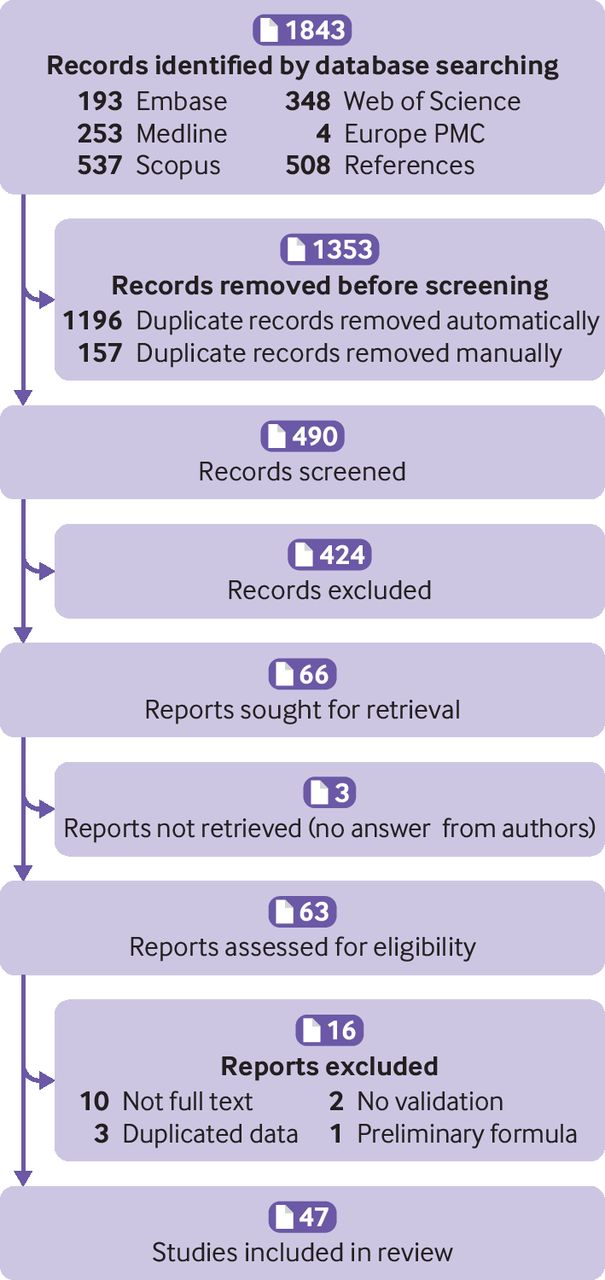
\includegraphics[scale=1]{figures/ADNEXSR/F1.jpg}
\caption[PRISMA flowchart]{PRISMA (Preferred Reporting Items for Systematic Reviews and Meta-Analyses) flowchart of study inclusions and exclusions.}
\label{fig:1:1}
\end{figure}



We identified 1843 records and screened 490 after de-duplication. Forty-seven
studies met our inclusion criteria and were included in this systematic review
(Figure \ref{fig:1:1}, Table S3)
 \cite{vancalsterValidationModelsDiagnose2020,
hackExternalValidationORADS2022,
jeongValidationIOTAADNEXModel2020,
quarantaSurgeryBenignOvarian2020,
araujoPerformanceIOTAADNEX2017,
behnamfarComparisonUltrasoundTumor2022,
budianaSkorAssessmentDifferent2022,
butureanuOvarianMassesapplicableIota2021,
chenComparisonORADSADNEX2022,
chenPerformanceIOTAADNEX2019,
czekierdowskiSonographicAssessmentComplex2021,
czekierdowskiPerformanceIOTASimple2023,
diazOvarianTumorsRisk2017a,
epsteinSubjectiveUltrasoundAssessment2016,
esquivelvillabonaTwoStepStrategyOptimizing2022,
gaurilcikasPerformanceIOTAADNEX2020,
heEstimatingRiskMalignancy2021,
hiettPerformanceIOTASimple2022,
huComparisonUltrasoundbasedADNEX2023,
jiangOvarianSexCord2021,
jianhongComparisonPerformanceORADS2022,
joyeuxSurgeryPredictabilityMalignant2016,
laiComparisonORADSGIRADS2022,
lamhuongOptimalCutOffPoint2022,
leeUltrasonographicEvaluationOvarian2021,
liuADNEXModelbasedDiagnosis2021,
meysEstimatingRiskMalignancy2017,
namAssessmentDifferentNEoplasias2021,
nohuzReliabilityIOTAScore2019,
pelayoComparisonUltrasoundScores2023,
pengEvaluationDiagnosticValue2021,
poonyakanokPreoperativeEvaluationADNEX2021,
qianComparisonDiagnosticPerformances2021,
rashmiDiagnosticPerformanceUltrasoundBased2023,
sandalComparisionRiskMalignancy2018a,
sayasnehEvaluatingRiskOvarian2016,
stukanDevelopmentValidationModel2019,
stukanUltrasoundClinicalPreoperative2019,
szubertExternalValidationIOTA2016,
szubertPerformanceSelectedModels2020,
tavoraiteUltrasoundAssessmentAdnexal2021,
tugPreoperativeDiscriminatingPerformance2020,
velayoDiagnosticPerformancesUltrasoundBased2023,
vioraADNEXModelTriage2020,
wangEvaluatingRiskMalignancy2023,
yangPerformanceIOTAADNEX2022,
zhangExternalValidationAssessment2022}.
Three studies were excluded because they used the same data as in another
included study, and one study was excluded because a preliminary formula of
\gls{ADNEX} was used
 \cite{landolfoBenignDescriptorsADNEX2023,
poonyakanokProspectiveComparativeTrial2023,
froymanRiskComplicationsPatients2019,
wynantsClinicalUtilityRisk2017}.
The data of three studies that were \gls{IOTA}-linked and three other studies with a
potential conflict of interest were extracted by authors PD and GSC
 \cite{vancalsterValidationModelsDiagnose2020,
epsteinSubjectiveUltrasoundAssessment2016,
meysEstimatingRiskMalignancy2017,
sayasnehEvaluatingRiskOvarian2016,
stukanDevelopmentValidationModel2019,
szubertPerformanceSelectedModels2020}.




Key study characteristics are summarised in Table \ref{tab:1} (Table S3 shows
study-specific details). The unit of analysis was the patient in 42 (89\%)
studies and the tumour in five (11\%) studies. When tumour was the unit of
analysis, multiple tumours for the same patient could be included. The 47
studies reported on 17007 tumours, with a median study sample size of 261
tumours (range 24 to 4905). The validations were conducted in 28 countries with
most studies being conducted in Asia (51\%) and Europe (38\%). Supplementary
Material S7 presents a list of reporting inconsistencies. All studies classified
borderline tumours as malignant tumours.



\gls{ADNEX} with CA125 was validated in 37 (79\%) studies, and \gls{ADNEX} without CA125 in
19 (40\%) studies (16 studies evaluated both versions). Three (6\%) studies
conducted a mixed validation, using \gls{ADNEX} with CA125 when CA125 was available.
For four (9\%) studies, the \gls{ADNEX} version was unclear. In total, 63 validations
of \gls{ADNEX} were performed after distinguishing between the \gls{ADNEX} versions used
(Table S4). When also including reported results for subgroups (e.g., by
menopausal status, or by centre in multicentre studies), the total number of
validations reported across the 47 studies was 159. Five (11\%) studies focused
only on a specific clinical subgroup, such as pregnant women or tumours for
which the clinician’s subjective assessment of the outcome was uncertain
 \cite{quarantaSurgeryBenignOvarian2020,
  czekierdowskiSonographicAssessmentComplex2021,
  leeUltrasonographicEvaluationOvarian2021,nohuzReliabilityIOTAScore2019,
  szubertPerformanceSelectedModels2020}.
Eight (17\%) studies selected patients based on histology (Table S3 for
details).

\begin{sidewaystable}[h!]
\centering
\caption[Meta-analysis of AUC]{Meta-analysis of the AUC to discriminate between benign and malignant tumours, including sensitivity and subgroup analyses.}
\label{tab:2}
\footnotesize
\begin{tabularx}{\textheight}{>{\raggedright\arraybackslash}X c c c c}
\toprule
\textbf{Meta-analysis} & \textbf{Studies (centres)} & \textbf{Summary estimate (95\% \gls{CI})} & \textbf{95\% PI} & \textbf{$\tau^2$} \\
\midrule
\textbf{Main analysis} & & & & \\
Operated patients, with CA125 & 21~(43) & 0.93~(0.92-0.94) & 0.85~to~0.98 & 0.25 \\
Operated patients, without CA125 & 12~(31) & 0.93~(0.91-0.94) & 0.85~to~0.98 & 0.21 \\
\addlinespace
\textbf{Sensitivity analyses (operated patients)} & & & & \\
High or Unclear risk of bias studies, with CA125 & 19~(23) & 0.93~(0.91-0.95) & 0.84~to~0.99 & 0.33 \\
Low risk of bias studies, with CA125 & 2~(20) & 0.93~(0.91-0.94) & 0.87~to~0.97 & 0.12 \\
\gls{IOTA} studies, with CA125 & 4~(23) & 0.92~(0.91-0.94) & 0.88~to~0.97 & 0.09 \\
Non-\gls{IOTA} studies, with CA125 & 17~(20) & 0.93~(0.91-0.95) & 0.83~to~0.99 & 0.38 \\
High or Unclear risk of bias studies, without CA125 & 10~(11) & 0.94~(0.92-0.96) & 0.86~to~0.99 & 0.26 \\
Low risk of bias studies, without CA125 & 2~(20) & 0.91~(0.90-0.93) & 0.85~to~0.96 & 0.11 \\
\gls{IOTA} studies, without CA125 & 2~(20) & 0.91~(0.89-0.93) & 0.85~to~0.97 & 0.14 \\
Non-\gls{IOTA} studies, without CA125 & 10~(11) & 0.94~(0.92-0.96) & 0.86~to~0.99 & 0.26 \\
\addlinespace
\textbf{Subgroup analyses (operated patients)} & & & & \\
Asian centres, with CA125 & 11~(13) & 0.94~(0.91-0.96) & 0.81~to~>0.99 & 0.54 \\
Asian centres, without CA125 & 7~(8) & 0.95~(0.93-0.97) & 0.89~to~0.99 & 0.19 \\
Chinese centres, with CA125 & 5~(5) & 0.94~(0.91-0.97) & 0.87~to~0.99 & 0.25 \\
Chinese centres, without CA125 & 4~(4) & 0.94~(0.90-0.97) & 0.85~to~0.99 & 0.33 \\
European centres, with CA125 & 8~(28) & 0.92~(0.91-0.94) & 0.88~to~0.96 & 0.07 \\
European centres, without CA125 & 3~(21) & 0.91~(0.89-0.93) & 0.84~to~0.97 & 0.16 \\
Non-oncology centres, with CA125 & 2~(9) & 0.91~(0.88-0.94) & 0.85~to~0.97 & 0.11 \\
Non-oncology centres, without CA125 & 1~(8) & 0.90~(0.86-0.95) & 0.80~to~0.99 & 0.24 \\
Oncology centres, with CA125 & 18~(31) & 0.93~(0.92-0.95) & 0.84~to~0.98 & 0.29 \\
Oncology centres, without CA125 & 12~(23) & 0.93~(0.91-0.94) & 0.85~to~0.98 & 0.22 \\
Postmenopausal patients, with CA125 & 11~(32) & 0.92~(0.90-0.94) & 0.83~to~0.98 & 0.25 \\
Postmenopausal patients, without CA125 & 4~(22) & 0.90~(0.87-0.93) & 0.81~to~0.97 & 0.19 \\
Premenopausal patients, with CA125 & 11~(32) & 0.91~(0.89-0.94) & 0.81~to~0.98 & 0.28 \\
Premenopausal patients, without CA125 & 4~(22) & 0.91~(0.89-0.93) & 0.85~to~0.96 & 0.08 \\
\addlinespace
\textbf{Target population\textsuperscript{a}} & & & & \\
Operated and non-surgically managed patients, with CA125 & 2~(18) & 0.94~(0.93-0.96) & 0.88~to~0.99 & 0.22 \\
Operated and non-surgically managed patients, without CA125 & 1~(17) & 0.94~(0.91-0.95) & 0.82~to~0.98 & 0.27 \\
\bottomrule
\addlinespace[0.5em]
\multicolumn{5}{l}{\textsuperscript{a}Follow up time was 10-14 months (1 year) or 2 years}
\end{tabularx}
\end{sidewaystable}



Thirty-six (77\%) studies did not focus on a specific clinical subgroup and did
not select tumours based on histology. In these 36 studies that were eligible
for the meta-analysis, the median sample size was 284 tumours (range 50-4905),
the median number of malignant tumours was 68 (7-1041) and the median prevalence
of malignancy 28\% (3\%-57\%). Fourteen of the 36 (39\%) studies had at least
100 benign and at least 100 malignant tumours. The target population of the
studies could be surgically managed patients or surgically and non-surgically
managed patients. The reference standard for determining the tumour type in
surgically managed patients was always histopathology. Four (9\%) studies
included surgically and non-surgically managed patients. In non-surgically
managed patients, the outcome determination was the clinician’s subjective
assessment of the tumour as benign or malignant or spontaneous resolution of the
tumour during follow-up. The required follow-up time to determine the outcome
was 3-4 months, 1 year, or 2 years, depending on the study
 \cite{vancalsterValidationModelsDiagnose2020,hackExternalValidationORADS2022,
  jeongValidationIOTAADNEXModel2020,quarantaSurgeryBenignOvarian2020}.

The most commonly reported performance measure was the \gls{AUC} for benign vs
malignant tumours (72\%) (Table S5). About two-thirds of studies (66\%)
presented a receiver operating characteristic curve, 31 (66\%) reported
sensitivity and specificity performance at the 10\% threshold for the risk of
malignancy, 12 (26\%) reported measures for multinomial discrimination and four
(9\%) studies reported calibration performance.

\subsection{Critical appraisal: reporting and risk of bias}
Completeness of reporting the \gls{TRIPOD} items was assessed for the 63 validations.
Adherence to \gls{TRIPOD} items was on average 61\%: studies reported on average 16.5
out of 27 items (Figures \ref{fig:1:2} and S1). The least commonly reported items were
‘comparison of demographics, predictors and outcome between the model
development and external validation data’ (item 13c; 5\%), ‘the reporting of
performance measures with confidence intervals’ (item 16; 11\%), ‘specification
of all performance measures’ (item 10d; 11\%), ‘rationale for study sample size’
(item 8; 13\%), and ‘description of how missing data were handled’ (item 9;
22\%).
\begin{figure}
\centering
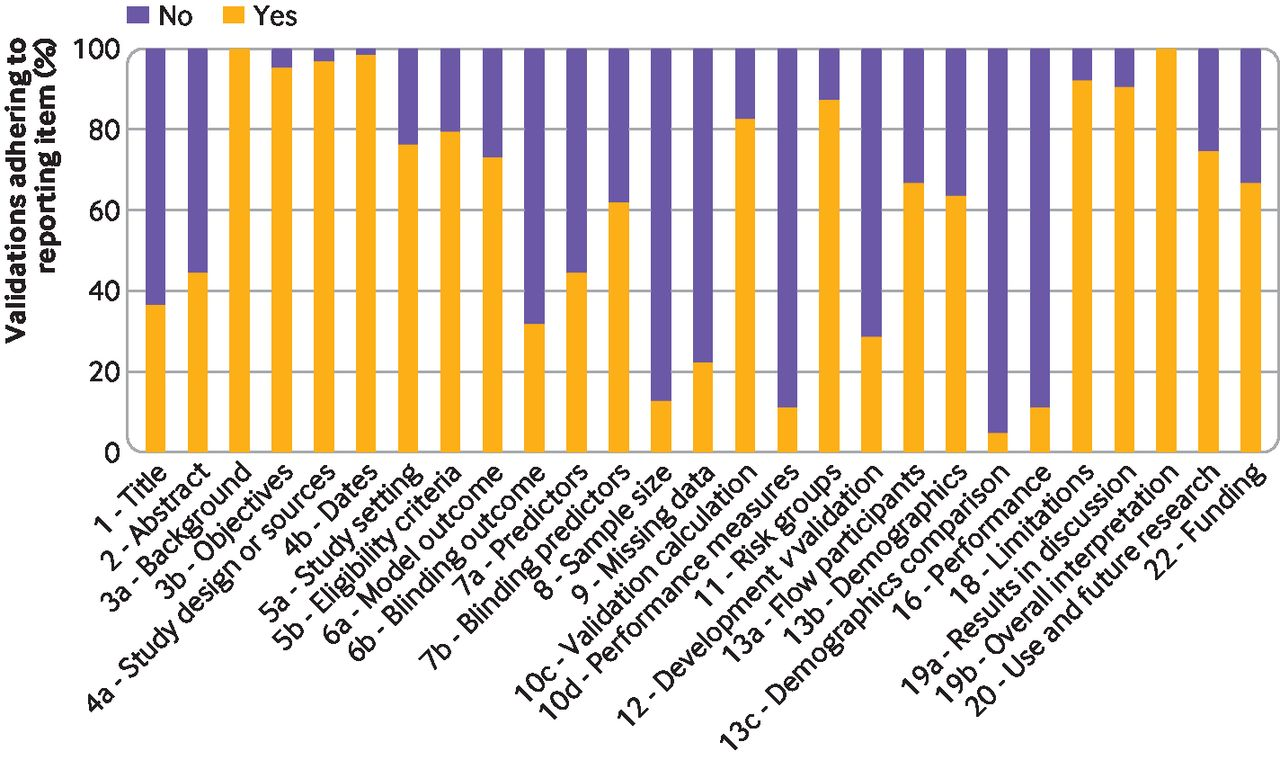
\includegraphics[width=0.8\textwidth]{figures/ADNEXSR/F2.large.jpg}
\caption[Adherence to TRIPOD]{Adherence to reporting the TRIPOD (Transparent Reporting of a multivariable prediction model for Individual Prognosis Or Diagnosis) items in 63 validations.}
\label{fig:1:2}
\end{figure}

\begin{figure}
\centering
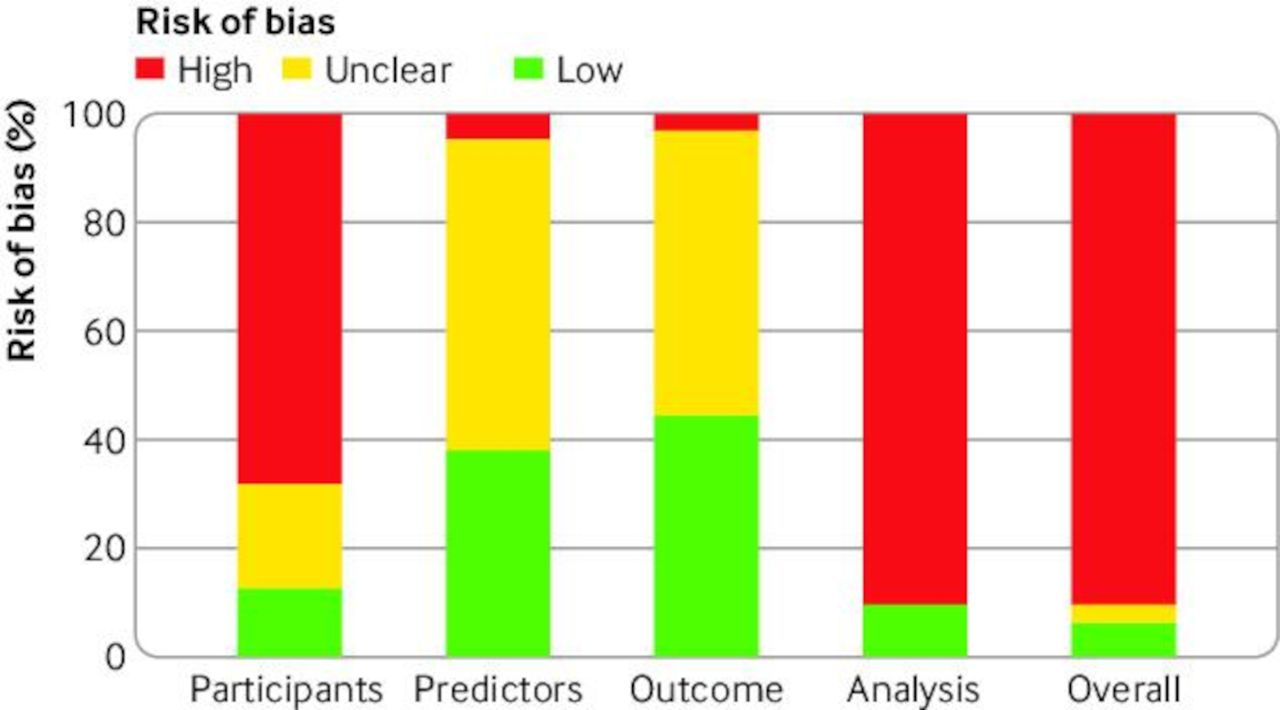
\includegraphics[width=0.8\textwidth]{figures/ADNEXSR/F3.large.jpg}
\caption[Risk of bias overall and by subdomain in 63 validations, assessed by PROBAST]{Risk of bias overall and by subdomain in 63 validations, assessed by PROBAST (Prediction model Risk Of Bias Assessment Tool).}
\label{fig:1:3}
\end{figure}
Fifty-seven (90\%) of 63 validations were rated at high risk of bias, two (3\%)
at uncertain risk of bias, and four (6\%) at low risk of bias (Figures \ref{fig:1:3}, S2-5,
\gls{OSF} Extraction sheet) \cite{barrenadaADNEXRiskModel2025}. 43 (68\%) validations
were at high risk of bias for the participant domain, mostly by having
incomplete data as an exclusion criterion. Fifty-seven (90\%) validations were
at high risk of bias for the analysis domain, mostly due to small sample size
(69\%; i.e. less than 100 tumours in the smallest group), not including all
participants in the analysis (85\%), inappropriate handling of missing data
(82\%), and incomplete evaluation of model performance - in most instances by
not reporting an assessment of calibration (89\%).

\gls{TRIPOD} adherence in 36 studies without focus on selected histologies or clinical
subgroups was on average 65\% (17.47 items out of 27). In these studies, two
where at low risk of bias, one at unclear risk of bias and 33 at high risk of
bias.

\subsection{Meta-analysis}
The meta-analysis included studies without post hoc selection based on histology
and without focus on a clinical subgroup only (n = 36) that reported the
meta-analysed metrics. Just two studies included in the meta-analysis used
tumour as unit of study
 \cite{behnamfarComparisonUltrasoundTumor2022,esquivelvillabonaTwoStepStrategyOptimizing2022}.

The \gls{AUC} for benign vs malignant tumours in operated patients was reported in 12
studies (6309 tumours, 31 centres, 13 countries) for \gls{ADNEX} without CA125 (Table
S4 and S6), and the summary \gls{AUC} was 0.93 (\gls{CI} 95\% 0.91-0.94, 95\% \gls{PI} 0.85-0.98)
(Table \ref{tab:2}, Figure \ref{fig:1:4})
 \cite{vancalsterValidationModelsDiagnose2020,chenComparisonORADSADNEX2022,
  diazOvarianTumorsRisk2017a,heEstimatingRiskMalignancy2021,
  hiettPerformanceIOTASimple2022,lamhuongOptimalCutOffPoint2022,
  pelayoComparisonUltrasoundScores2023,pengEvaluationDiagnosticValue2021,
  poonyakanokPreoperativeEvaluationADNEX2021,
  qianComparisonDiagnosticPerformances2021,
  sayasnehEvaluatingRiskOvarian2016,
  zhangExternalValidationAssessment2022}.
Twenty-one studies (9202 tumours, 43 centres, 18 countries) reported the \gls{AUC} for
benign vs malignant tumours in operated patients for \gls{ADNEX} with CA125,
 \cite{vancalsterValidationModelsDiagnose2020,araujoPerformanceIOTAADNEX2017,
  behnamfarComparisonUltrasoundTumor2022,chenPerformanceIOTAADNEX2019,
  diazOvarianTumorsRisk2017a,heEstimatingRiskMalignancy2021,
  joyeuxSurgeryPredictabilityMalignant2016,
  lamhuongOptimalCutOffPoint2022,meysEstimatingRiskMalignancy2017,
  namAssessmentDifferentNEoplasias2021,pengEvaluationDiagnosticValue2021,
  poonyakanokPreoperativeEvaluationADNEX2021,
  qianComparisonDiagnosticPerformances2021,
  sayasnehEvaluatingRiskOvarian2016,stukanDevelopmentValidationModel2019,
  szubertPerformanceSelectedModels2020,szubertExternalValidationIOTA2016,
  tugPreoperativeDiscriminatingPerformance2020,vioraADNEXModelTriage2020,
  yangPerformanceIOTAADNEX2022,zhangExternalValidationAssessment2022}
(Table S4 and S6) and the summary \gls{AUC} was 0.93 (\gls{CI} 95\% 0.92-0.94, 95\% \gls{PI}
0.85-0.98) (Table \ref{tab:2}, Figure \ref{fig:1:5}).

\begin{figure}
\flushleft
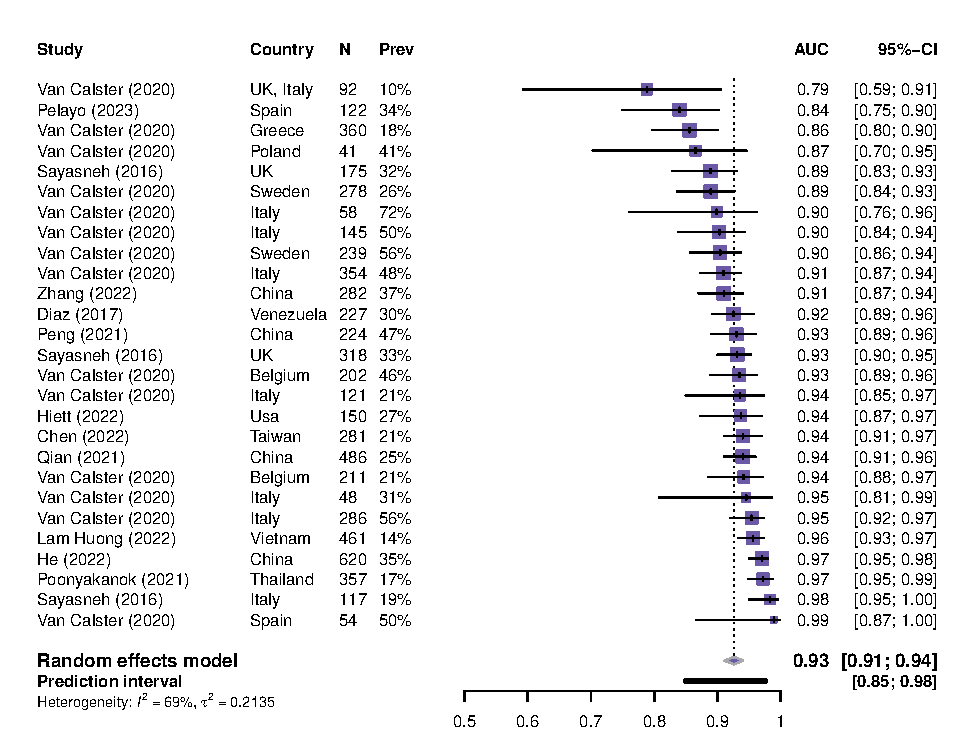
\includegraphics[width=1\textwidth]{figures/ADNEXSR/Figure4.pdf}
\caption[Forest plot AUC ADNEX without CA125]{Forest plot of area under the receiver operating curve in studies where the ADNEX (Assessment of Different Neoplasias in the adnexa) model was used without CA125 (cancer antigen 125). Results in the forest plot are centre specific results, so studies with more than one centre can appear multiple times. CI=confidence interval}
\label{fig:1:4}
\end{figure}

\begin{figure}
\flushleft
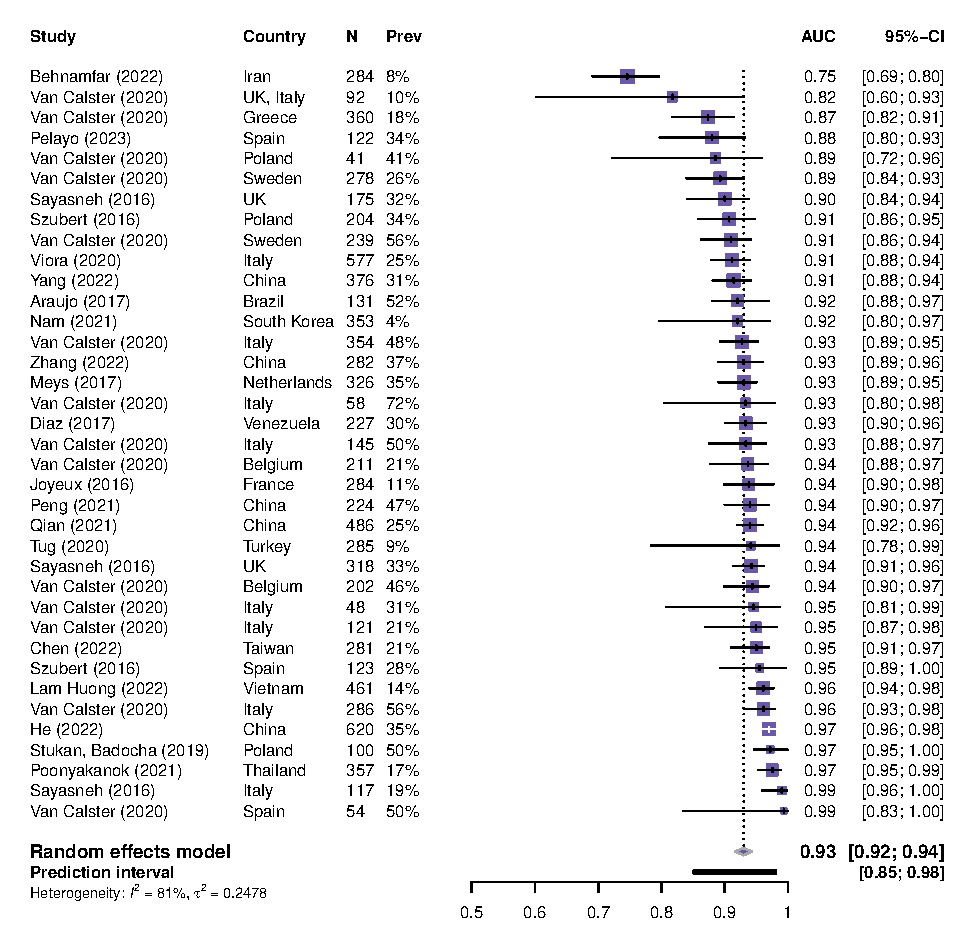
\includegraphics[width=1\textwidth]{figures/ADNEXSR/Figure5.pdf}
\caption[Forest plot AUC ADNEX with CA125]{Forest plot of area under the receiver operating characteristic curve in studies where the ADNEX (Assessment of Different Neoplasias in the adnexa) model was used with CA125 (cancer antigen 125). Results in the forest plot are centre specific results, so studies with more than one centre can appear multiple times. CI=confidence interval}
\label{fig:1:5}
\end{figure}




Sensitivity and specificity at the 10\% risk of malignancy threshold in operated
patients were reported in ten studies for \gls{ADNEX} without CA125 (Tables S4 and S7)
 \cite{vancalsterValidationModelsDiagnose2020,chenComparisonORADSADNEX2022,
  diazOvarianTumorsRisk2017a,hiettPerformanceIOTASimple2022,
  lamhuongOptimalCutOffPoint2022,pelayoComparisonUltrasoundScores2023,
  poonyakanokPreoperativeEvaluationADNEX2021,
  qianComparisonDiagnosticPerformances2021,
  sayasnehEvaluatingRiskOvarian2016,
  zhangExternalValidationAssessment2022}.
The summary sensitivity and specificity were 0.93 (95\% \gls{CI} 0.90-0.95, 95\% \gls{PI}
0.73-0.99) and 0.75 (95\% \gls{CI} 0.70-0.79, 95\% \gls{PI} 0.46-0.91), respectively (Table
S8, Figure \ref{fig:1:6}). For \gls{ADNEX} with CA125, sensitivity and specificity at the 10\%
risk of malignancy threshold in operated patients were reported in 24 studies
(Tables S4 and S7)
 \cite{vancalsterValidationModelsDiagnose2020,
  jeongValidationIOTAADNEXModel2020,araujoPerformanceIOTAADNEX2017,
  chenComparisonORADSADNEX2022,diazOvarianTumorsRisk2017a,
  heEstimatingRiskMalignancy2021,
  joyeuxSurgeryPredictabilityMalignant2016,laiComparisonORADSGIRADS2022,
  lamhuongOptimalCutOffPoint2022,meysEstimatingRiskMalignancy2017,
  namAssessmentDifferentNEoplasias2021,
  pelayoComparisonUltrasoundScores2023,pengEvaluationDiagnosticValue2021,
  poonyakanokPreoperativeEvaluationADNEX2021,
  qianComparisonDiagnosticPerformances2021,
  sandalComparisionRiskMalignancy2018a,sayasnehEvaluatingRiskOvarian2016,
  stukanDevelopmentValidationModel2019,szubertExternalValidationIOTA2016,
  tugPreoperativeDiscriminatingPerformance2020,vioraADNEXModelTriage2020,
  wangEvaluatingRiskMalignancy2023,yangPerformanceIOTAADNEX2022,
  zhangExternalValidationAssessment2022}.
The summary sensitivity and specificity were 0.94 (\gls{CI} 95\% 0.92-0.95; 95\% \gls{PI}
0.80-0.98) and 0.77 (\gls{CI} 95\% 0.73-0.81; 95\% \gls{PI} 0.47-0.93, respectively (Table
S8, Figure \ref{fig:1:7}).

\gls{NB} and \gls{RU} were calculated using studies that presented sensitivity and
specificity at the 10\% risk of malignancy threshold in operated patients (Table
S7). For \gls{ADNEX} without CA125, the summary \gls{NB} was 0.28 (95\% \gls{CrI} 0.22-0.35, 95\%
\gls{PI} 0.05-0.67) and the summary \gls{RU} 0.50 (95\% \gls{CrI} 0.36-0.62, 95\% \gls{PI} -0.41-0.81).
The probability that the model is clinically useful in a random new centre was
estimated to be 91\% (Table S9, Figures S6-7). For \gls{ADNEX} with CA125, the summary
\gls{NB} was 0.27 (95\% \gls{CrI} 0.23-0.33, 95\% \gls{PI} 0.06-0.64) and the summary \gls{RU} 0.54
(95\% \gls{CrI} 0.45-0.61, 95\% \gls{PI} -0.12-0.78). The probability that the model is
clinically useful in a random new centre was estimated to be 95\% (Table S9,
Figures S8-9).

Pairwise \glspl{AUC} in operated patients were reported in 4 studies for \gls{ADNEX} without
CA125 and in 5 studies for \gls{ADNEX} with CA125 (Table S10)
 \cite{vancalsterValidationModelsDiagnose2020,
  poonyakanokPreoperativeEvaluationADNEX2021,
  sayasnehEvaluatingRiskOvarian2016,vioraADNEXModelTriage2020,
  zhangExternalValidationAssessment2022}.
The summary pairwise \glspl{AUC} for \gls{ADNEX} without CA125 ranged from 0.66 (stage II-IV
primary invasive vs metastatic) to 0.97 (benign vs stage II-IV primary invasive)
(Table S11). For \gls{ADNEX} with CA125, the summary pairwise \glspl{AUC} ranged from 0.72
(borderline vs stage I primary invasive) to 0.98 (benign vs stage II-IV primary
invasive).

\begin{figure}
\flushleft
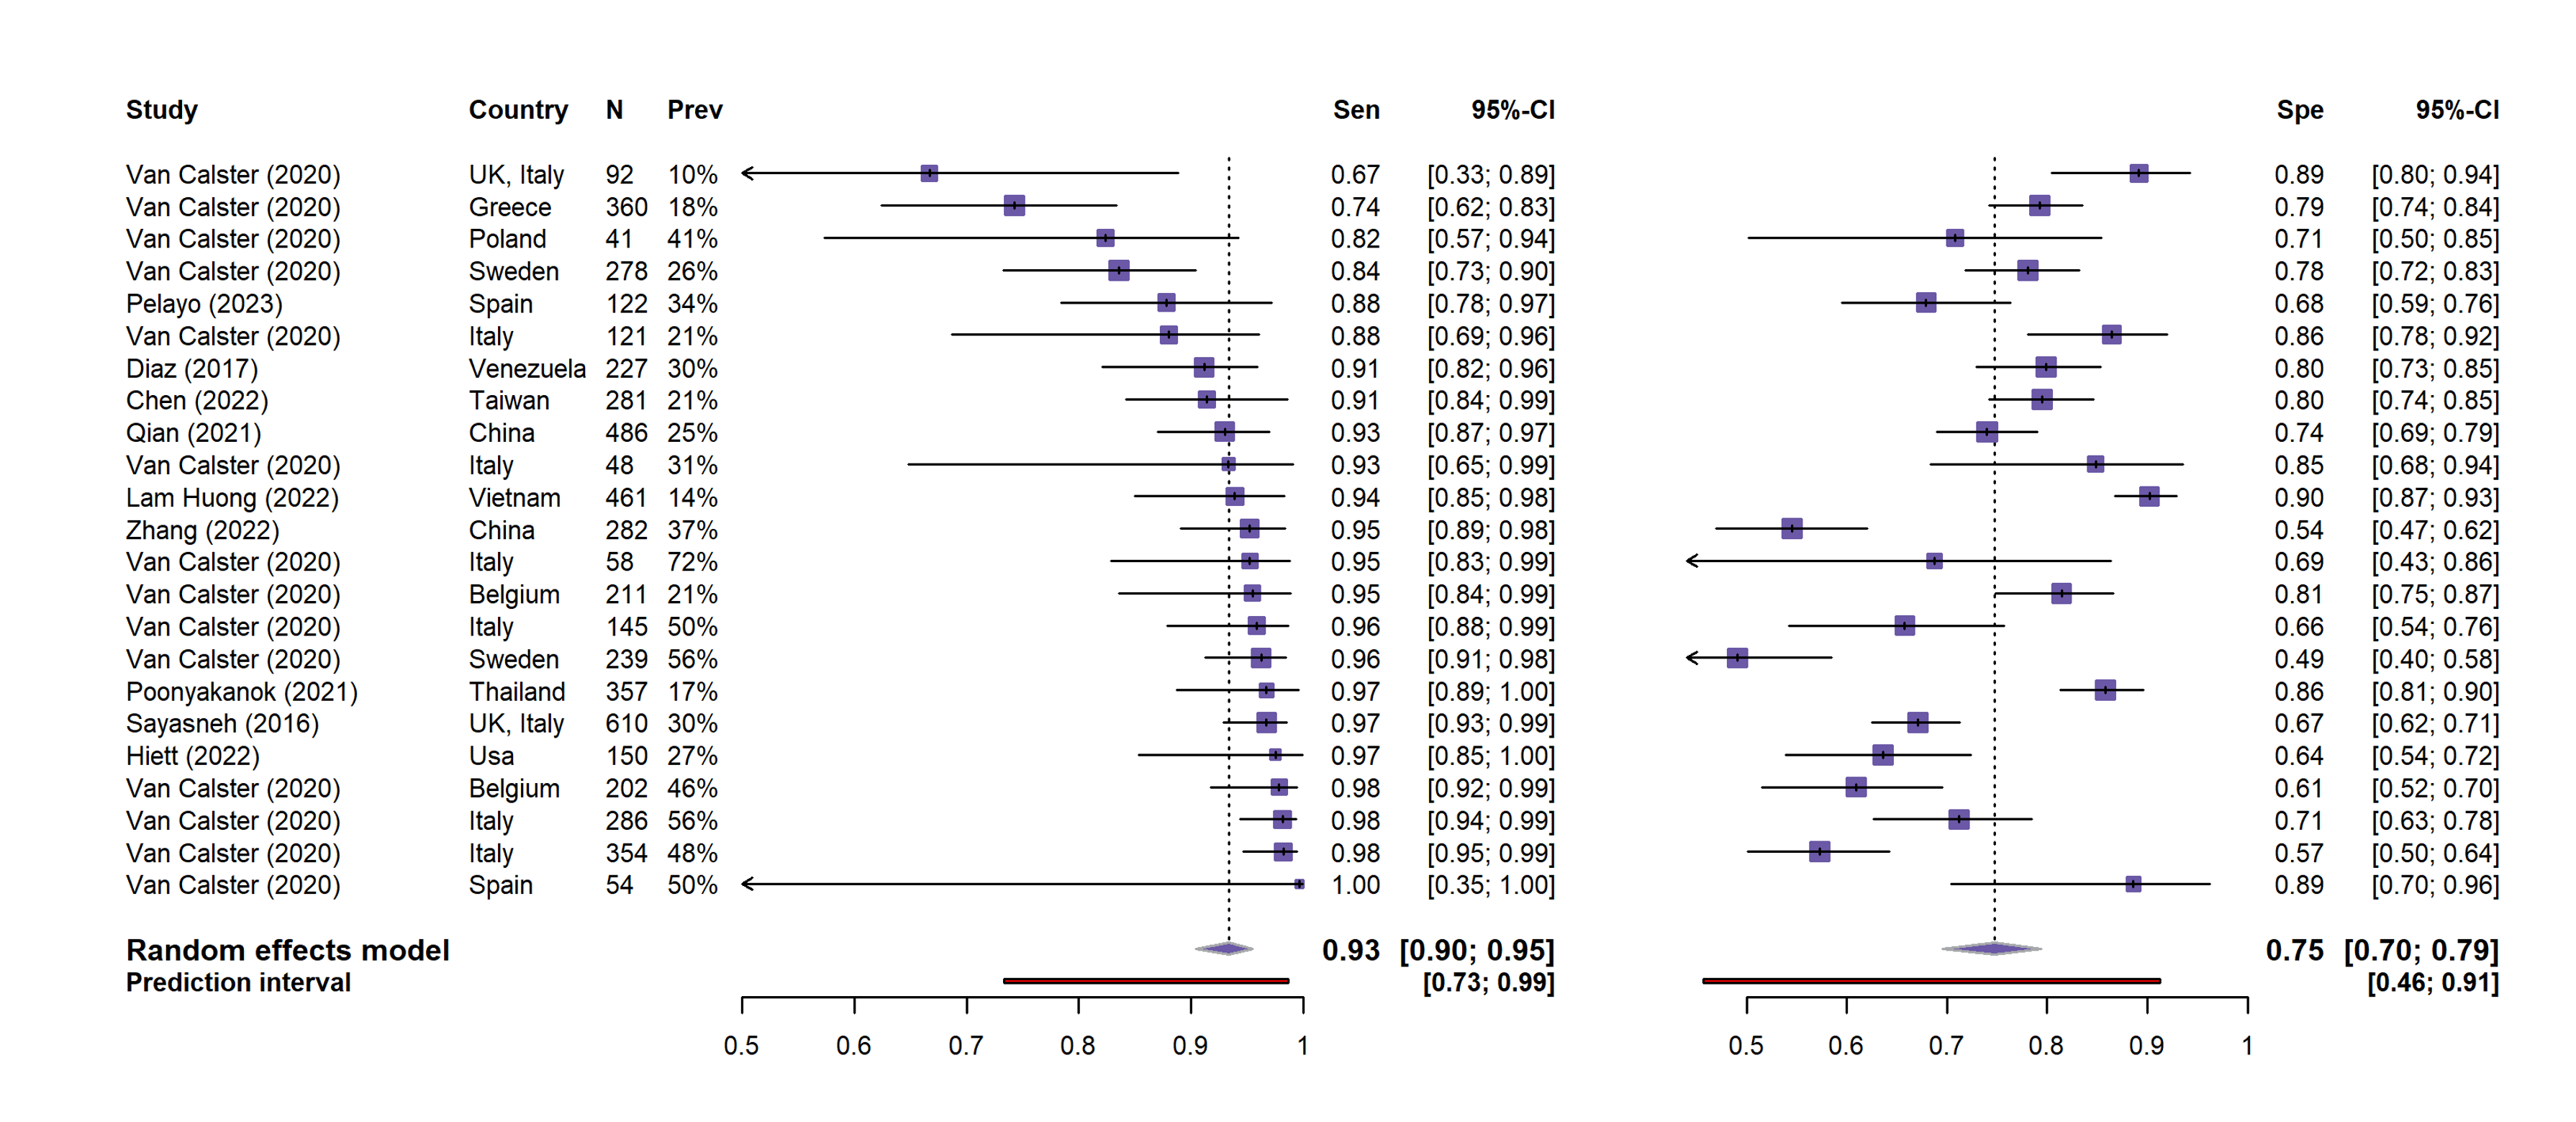
\includegraphics[width=1\textwidth]{figures/ADNEXSR/Figure6.png}
\caption[Forest plot sensitivity and specificity ADNEX without CA125 at 10\% risk of malignancy]{Forest plot of sensitivity and specificity at the 10\% risk of malignancy threshold in studies where the ADNEX (Assessment of Different Neoplasias in the adnexa) model was used without CA125 (cancer antigen 125). Results in the forest plot are centre specific results, so studies with more than one centre can appear multiple times. CI=confidence interval}
\label{fig:1:6}
\end{figure}

The \gls{AUC} for benign vs malignant tumours in operated and non-surgically managed
patients combined was reported in 2 studies (5167 tumours, 18 centres, 8
countries) with a summary estimate of 0.94 (95\% \gls{CI} 0.93-0.96, 95\% \gls{PI}
0.88-0.99) for \gls{ADNEX} with CA125 (Table \ref{tab:2})
 \cite{vancalsterValidationModelsDiagnose2020,hackExternalValidationORADS2022}.
\gls{ADNEX} without CA125 was assessed in only 1 study (4905 tumours, 17 centres, 7
countries) \cite{vancalsterValidationModelsDiagnose2020}. This study reported
summary \gls{AUC} 0.94 (95\% \gls{CI} 0.91-0.95, 95\% \gls{PI} 0.82-0.98).

Sensitivity and subgroup results for \gls{AUC}, specificity, sensitivity, \gls{NB} and \gls{RU}
are shown in Tables 2 and S6-9. These results showed that findings were robust
(\glspl{AUC} ranged from 0.90 to 0.95 across all analyses) and clinical utility was
suggested in all subgroups. When limiting the analyses to low RoB studies,
summary \glspl{AUC} were 0.93 (with CA125) and 0.91 (without CA125). Sensitivity was
higher and specificity lower in oncology versus non-oncology centres and in
postmenopausal versus premenopausal patients. In line with this, meta-regression
suggested that prevalence of malignancy was not related to \gls{AUC} but positively to
sensitivity and negatively to specificity (Figures S10-12).

\begin{figure}
\flushleft
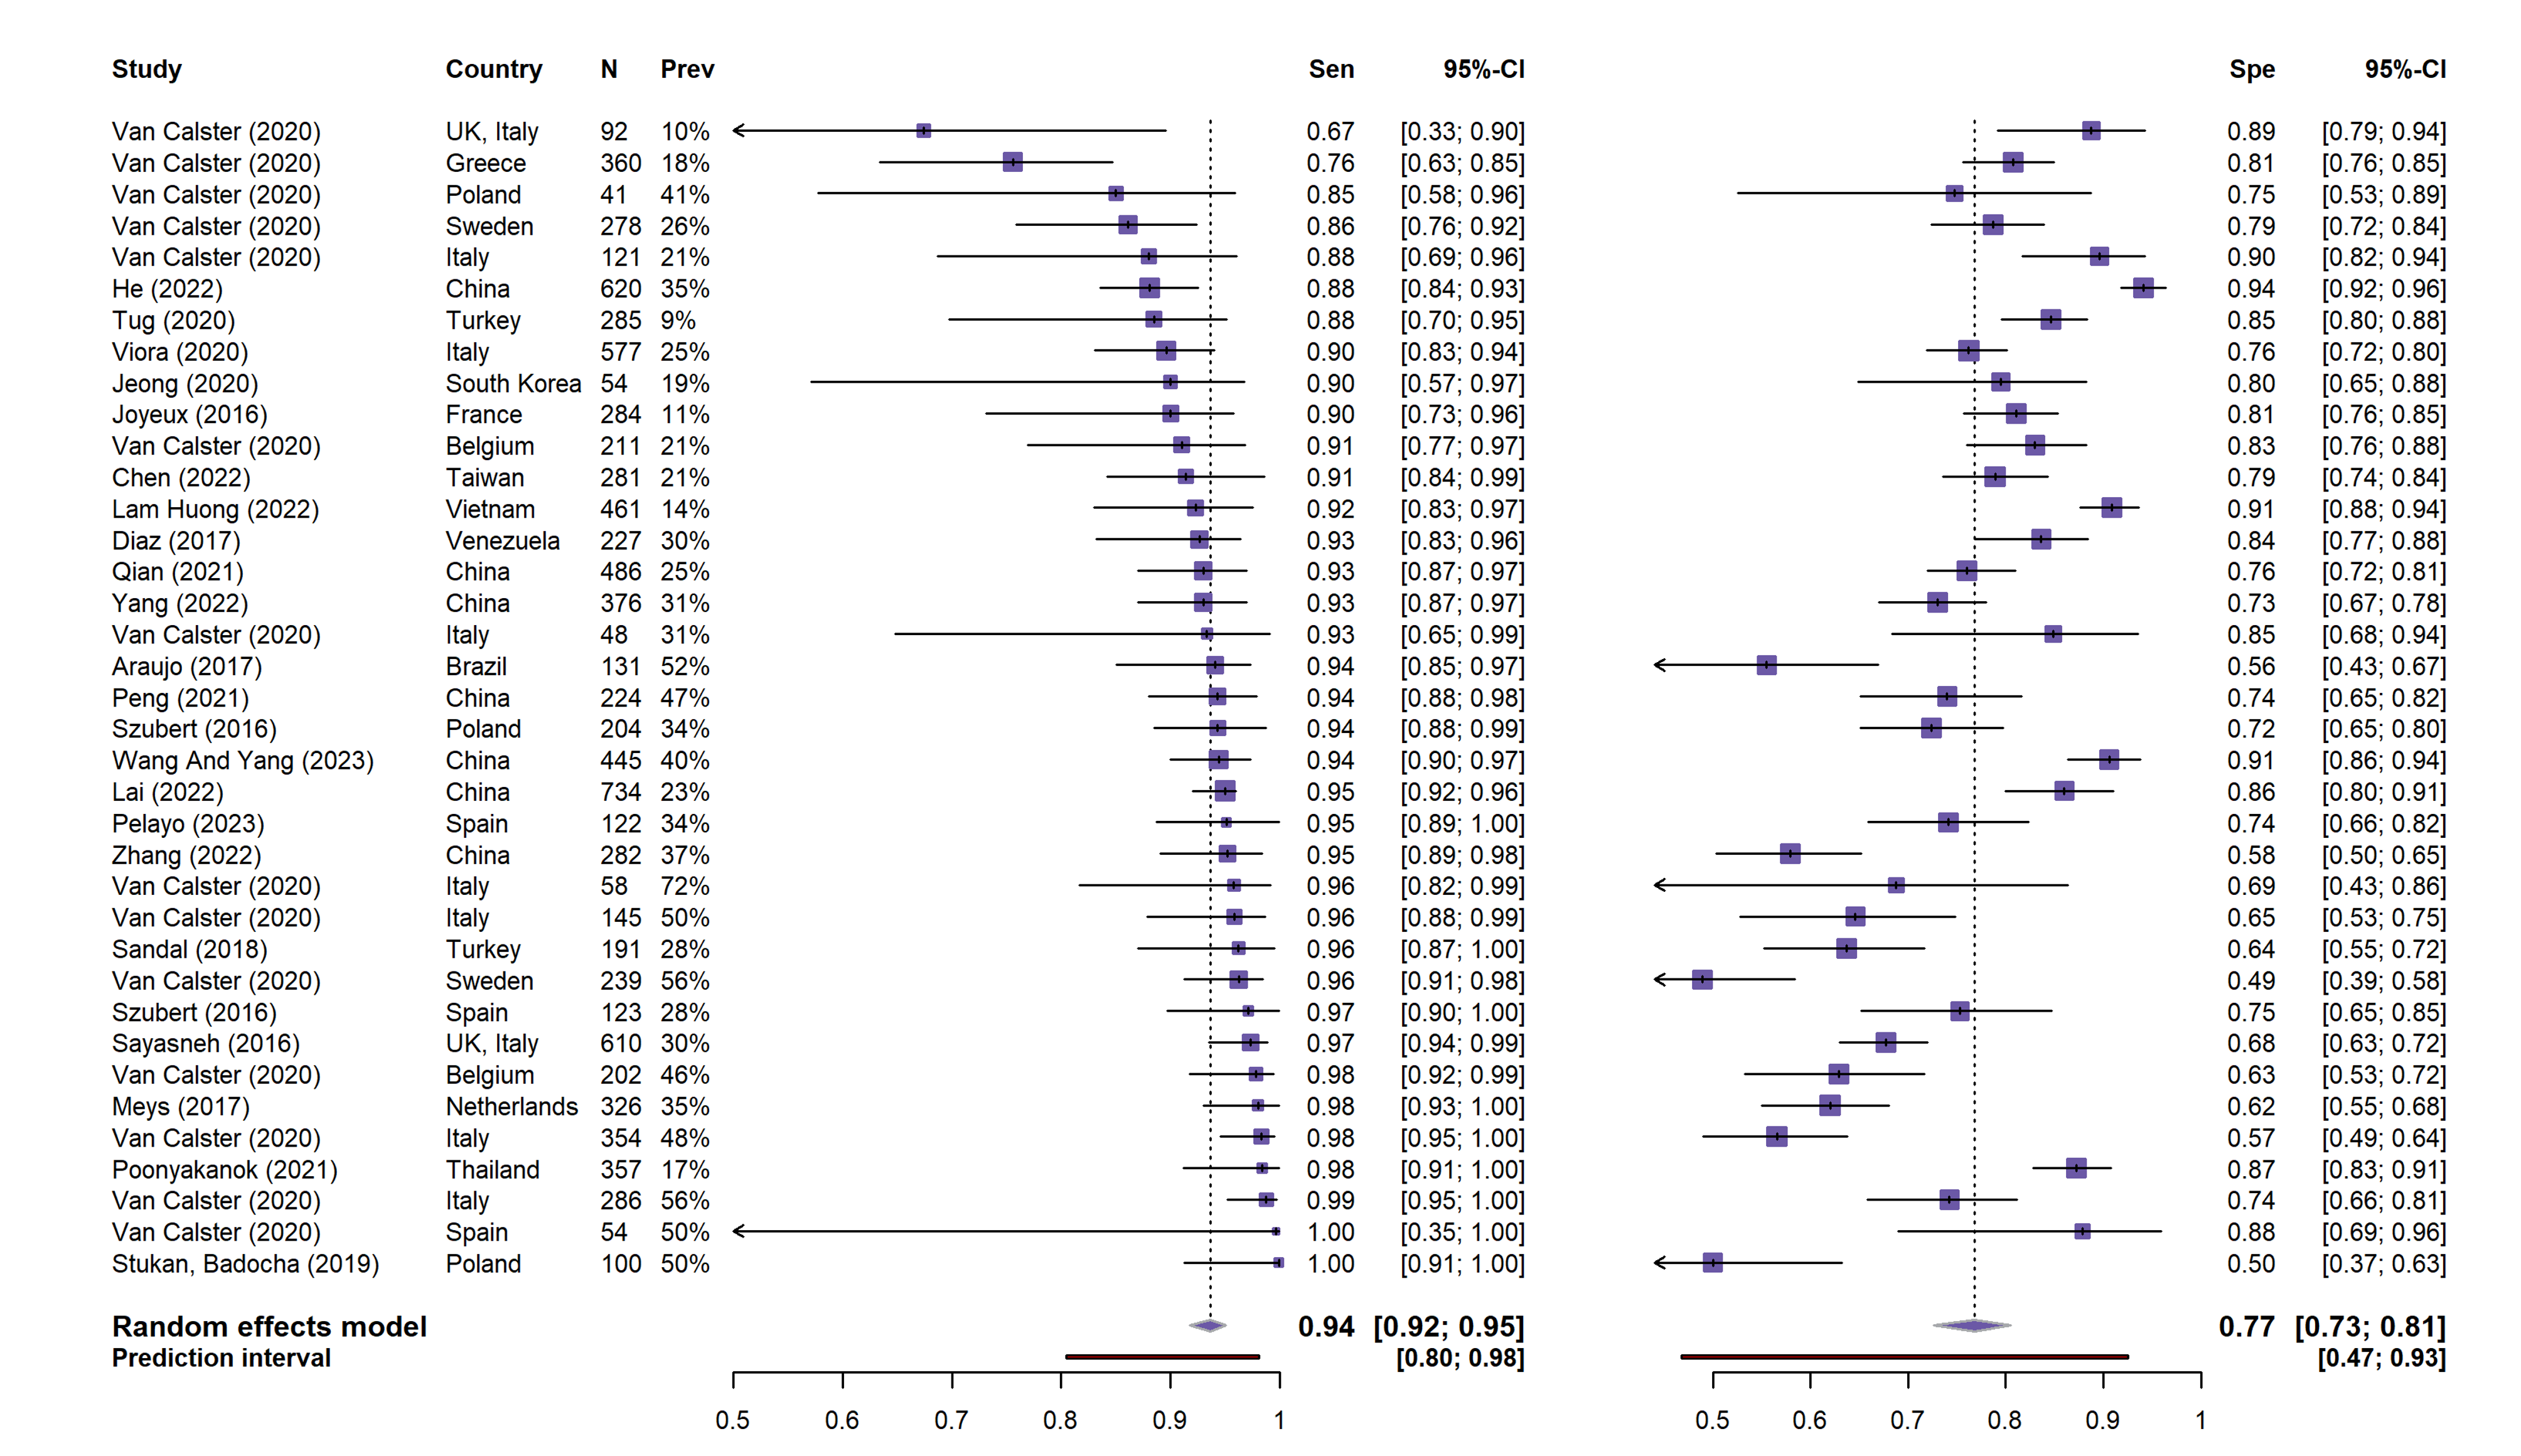
\includegraphics[width=1\textwidth]{figures/ADNEXSR/Figure7.png}
\caption[Forest plot sensitivity and specificity ADNEX with CA125 at 10\% risk of malignancy]{Forest plot of sensitivity and specificity at the 10\% risk of malignancy threshold in studies where the ADNEX (Assessment of Different Neoplasias in the adnexa) model was used with CA125 (cancer antigen 125). Results in the forest plot are centre specific results, so studies with more than one centre can appear multiple times. CI=confidence interval}
\label{fig:1:7}
\end{figure}



Meta-analysis of calibration in only operated patients was not feasible as only
one study reported calibration slope and intercept
 \cite{vancalsterValidationModelsDiagnose2020}. Four studies presented a
calibration plot: in three studies
 \cite{sayasnehEvaluatingRiskOvarian2016,vioraADNEXModelTriage2020,zhangExternalValidationAssessment2022}
the estimated risks were close to the observed ones, in one study
 \cite{vancalsterValidationModelsDiagnose2020} the risk of malignancy was
slightly underestimated (Supplementary material S8).

Based on the subdomains of \gls{GRADE} assessment, we have identified the risk of bias
in the studies included in this meta-analysis as a significant limitation
affecting the certainty of our meta-analysis results. Two studies (representing
5511 tumours or 32\% of total tumours included in this review) did not fall
under the classification of high risk of bias
 \cite{vancalsterValidationModelsDiagnose2020,sayasnehEvaluatingRiskOvarian2016}.
However, the sensitivity analysis according to risk of bias showed consistent
findings (Table \ref{tab:2}, Table S8 and S9). Funnel plots for the \gls{AUC} did not suggest
publication bias (Figure S13).

\section{Discussion}

The \gls{ADNEX} model exhibited robust discrimination and classification performance
between benign and malignant tumours across various settings and populations. In
addition, the results indicate that \gls{ADNEX} has clinical utility at the 10\% risk
of malignancy threshold, for example to help decide whether a patient should be
referred for assessment in a gynaecological oncology centre.

We found deficiencies in study reporting, and most studies were judged to be at
high risk of bias. However, our sensitivity analyses indicated that performance
was almost identical in low risk and high risk of bias studies. For \gls{ADNEX} with
CA125, the \gls{AUC} was 0.93 based on all studies vs 0.93 when based on only low risk
of bias studies. For \gls{ADNEX} without CA125, the \glspl{AUC} were 0.93 (all studies) and
0.91 (low risk of bias only). High risk of bias was mainly caused by low sample
size, absence of calibration performance, and unjustified use of complete case
analysis. Low sample size makes the estimated \gls{AUC} less precise but does not
systematically affect the \gls{AUC}, unless there is publication bias. The funnel
plots do not suggest publication bias. Absence of calibration does not affect
the \gls{AUC}. Using complete cases regarding CA125 or other predictors may lead to
underestimation of the \gls{AUC}, because missing values tend to be associated with
the examiner’s subjective impression that the tumour is benign
 \cite{landolfoBenignDescriptorsADNEX2023}. Complete case analysis would then
tend to exclude clearly benign tumours, which would make the sample more
homogeneous and reduce the \gls{AUC}. However, our results suggest that the impact of
complete case analysis on performance may have been minimal. The impact on
calibration could not be assessed. Taken together, the results presented in our
meta-analysis are reliable.

Strengths of our systematic review include the meta-analysis of \gls{ADNEX} both as a
risk model and as a diagnostic test, and the thorough critical appraisal
regarding risk of bias and reporting quality using recommended checklists
 \cite{wolffPROBASTToolAssess2019,collinsTransparentReportingMultivariable2015}.
Our study also has limitations. First, some study authors have a conflict of
interest because they were involved in developing \gls{ADNEX} or in some of the
included external validation studies. To address this, independent researchers
with expertise in study methodology and prediction modelling evaluated the
\gls{IOTA}-related studies. A limitation of our findings (but not of our study) is
that calibration performance was reported in only four studies so that
meta-analysis of calibration was not possible.

Previous systematic reviews have conducted meta-analyses of the diagnostic
performance of \gls{ADNEX} with CA125
 \cite{cuiDiagnosticAccuraciesUltrasound2022,
  davenportMenopausalStatusUltrasound2022,
  huangDiagnosticAccuracyADNEX2021,westwoodRiskScoresGuide2018,
  yueValueAssessmentDifferent2022}.
They used the \gls{QUADAS}-2 tool \cite{whitingQUADAS2RevisedTool2011} to assess risk
of bias, and found between 0 and 64\% of studies to be at high risk of bias in
at least one domain. We identified 45/47 studies as high risk of bias using the
\gls{PROBAST} tool designed for the appraisal of risk prediction models. None of the
previous meta-analyses of \gls{ADNEX} included clinical utility, calibration or \gls{AUC}.
Our results align with those of other systematic reviews of risk prediction
modelling studies in various domains. These consistently indicate that reporting
in the original studies was poor and that many studies were at high risk of bias
 \cite{collinsExternalValidationMultivariable2014,
  wynantsPredictionModelsDiagnosis2020,
  helmrichDoesPoorMethodological2022,
  dhimanReportingPrognosticClinical2021,andaurnavarroRiskBiasStudies2021,
  alloteyExternalValidationPrognostic2022,
  bouwmeesterReportingMethodsClinical2012}.
Still, the results in terms of sensitivity and specificity of \gls{ADNEX} in our
meta-analysis were similar to those in the other meta-analyses of \gls{ADNEX}
performance.

\gls{ADNEX} is intended for use by gynaecologists to help them decide on the most
appropriate management of an adnexal mass detected on ultrasound. Our findings
support the use of \gls{ADNEX} (1) to choose between surgery and conservative
follow-up, the latter in case of very low risk of malignancy, e.g. < 1\%
(meta-analysis in operated and non-surgically managed patients) (2) to decide on
the most appropriate management if conservative management is not suitable, e.g.
surgery at a local hospital if the risk of malignancy is less than 10\% or
referral to an oncology centre if the risk is >10\% (meta-analysis in operated
patients) \cite{timmermanESGOISUOGIOTA2021}. \gls{ADNEX} can also be helpful when
deciding on management of a suspected malignancy, i.e. investigations to find
the primary tumour if a metastasis in the ovary is likely, or fertility sparing
surgery if a borderline tumour is likely (meta-analysis in operated patients).
Because the \gls{AUC} of \gls{ADNEX} with and without CA125 are similar, and because adding
CA125 mainly helps to distinguish between different types of malignant tumours,
we argue that the main use of \gls{ADNEX} without CA125 is to help decide whether
conservative follow-up, surgery in a local centre or referral to an oncology
centre is appropriate. The main use of \gls{ADNEX} with CA125 is to help decide on
optimal management of a tumour suspected to be malignant, because it
differentiates better between malignant subtypes than \gls{ADNEX} without CA125.

While our findings suggest that \gls{ADNEX} has clinically utility, well conducted
validations of any model are always of value to monitor its performance in
diverse regions and clinical settings, and over time
 \cite{vancalsterThereNoSuch2023}. In line with this, to improve \gls{ADNEX}
performance even further, efforts to update the \gls{ADNEX} formula are of interest
 \cite{vancalsterThereNoSuch2023,
  onbehalfoftopicgroupevaluatingdiagnostictestsandpredictionmodelsofthestratosinitiativeCalibrationAchillesHeel2019}.
If further validation studies are conducted, we recommend to include a
validation of \gls{ADNEX} without CA125, to use a sufficiently large sample that
allows to assess calibration and multinomial discrimination, and to include
patients irrespective of whether they are managed surgically or non-surgically
(despite the challenges regarding reference standard for non-surgically managed
patients)
 \cite{vancalsterAssessingDiscriminativeAbility2012,vanhoordeAssessingCalibrationMultinomial2014}.
Methodological recommendations for validation studies include using available
tools to guarantee adequate sample size, describe missing data in detail and use
methods such as imputation when needed, and assess calibration performance
 \cite{steyerbergClinicalPredictionModels2009,
  onbehalfoftopicgroupevaluatingdiagnostictestsandpredictionmodelsofthestratosinitiativeCalibrationAchillesHeel2019,
  pateMinimumSampleSize2023,rileyMinimumSampleSize2021,
  siskImputationMissingIndicators2023}.
Finally, adherence to the \gls{TRIPOD} reporting checklists is important to maximise
the value of the validation study (www.tripod-statement.org).

\section{Conclusion}
\gls{ADNEX} has been widely validated with \gls{AUC} values >0.90 to discriminate between
benign and malignant tumours across various settings, and with strong results
regarding clinical utility at the 10\% risk of malignancy threshold. Due to lack
of calibration assessment in most studies, it was not possible to substantially
evaluate the accuracy of the estimated risks.

\section*{Acknowledgment}
The authors wish to thank Thomas Vandendriessche, Chayenne Van Meel and Krizia
Tuand, the biomedical reference librarians of the KU Leuven Libraries – 2Bergen
– learning Centre Désiré Collen (Leuven, Belgium), for their help in conducting
the systematic literature search. We gratefully acknowledge the authors of the
external validation of \gls{ADNEX} for providing their valuable data. This research
will be presented at \gls{ISUOG} World Congress 2023 in Seoul (October 2023).

\section*{Other information}
\subsection*{Funding}
This research was supported by the Research Foundation – Flanders (FWO) under
grant G097322N with BVC and DT as supervisors. LW and BVC were supported by
Internal Funds KU Leuven (grant C24M/20/064). JYV was supported by the National
Institute for Health and Care Research (NIHR) Community Healthcare MedTech and
In Vitro Diagnostics Co-operative at Oxford Health NHS Foundation Trust (N/A).
The views expressed are those of the author(s) and not necessarily those of the
NHS, the NIHR or the Department of Health and Social Care. GSC is supported by
Cancer Research UK (programme grant: C49297/A27294). PD is supported by CRUK
(project grant: PRCPJT-Nov21\textbackslash100021).

\subsection*{Conflicts of interest}
All authors have completed the ICMJE uniform disclosure form at
www.icmje.org/coi\_disclosure.pdf and declare: BVC, LV and DT are members of the
steering committee of the International Ovarian Tumour Analysis (\gls{IOTA})
consortium and were involved in the development of the \gls{ADNEX} model. BVC and DT
report consultancy work done by KU Leuven to help implementing and testing the
\gls{ADNEX} model in ultrasound machines by Samsung Medison, GE Healthcare, Canon
Medical Systems Europe, and Shenzhen Mindray Bio-medical Electronics, outside
the submitted work. GSC is a statistics editor for the BMJ. AL, LB, PD, LW and
JYV have nothing to declare.

\subsection*{Transparency declaration}
The lead authors affirm that this manuscript is an honest, accurate, and
transparent account of the study being reported; that no important aspects of
the study have been omitted; and that any discrepancies from the study as
planned (and, if relevant, registered) have been explained.

\subsection*{Availability of data and code}
Supplementary material is available online \cite{barrenadaADNEXRiskPrediction2024}.
The data and code used for the analysis and the generation of the figures is
publicly available in Open Science Framework (\url{https://osf.io/jtsvd/})
 \cite{barrenadaADNEXRiskModel2025}. This includes the extraction sheet, one
script for running the meta-analysis and one script for generating all the
figures included in the paper (except \gls{PRISMA} Flowchart). Note that for some rows
in the extraction sheet we deleted the performance measures for the menopausal
subgroups because this information was provided by authors upon request
therefore it is not publicly available.

\subsection*{Contributors}
Contributions were based on the CRediT taxonomy. Conceptualization: LB, BVC.
Funding acquisition: BVC, DT. Project administration: LB. Supervision: BVC.
Methodology: LB, GSC, LW, JYV, BVC. Resources: LB, AL. Investigation: LB, AL,
LV, BVC. Validation: LB, AL, PD, GSC, BVC. Data curation: LB, AL, JYV, LV, BVC.
Software: LB, LW, BVC. Formal analysis: LB, LW, BVC. Visualization: LB. Writing
– original draft: LB, BVC. Writing – review \& editing: all authors. All authors
have read, share final responsibility for the decision to submit for
publication, and agree to be accountable for all aspects of the work.

\subsection*{Ethics approval}
Not required because only secondary data from published studies were used.

\include{chapters/05.02_ADNEXvsRMI}
\chapter{ADNEX2}
\label{sec:chp_ADNEX2}
\includegraphics*[width=0.5\linewidth]{logos/medrxiv_logo.png}\vspace{0.5cm}

published as: 
\begin{quote}
Barreñada L et al. ADNEX2: Updating the ADNEX model to predict ovarian cancer for surgically and conservatively managed patients with an adnexal mass.  The British Medical Journal (BMJ) (submitted).
\end{quote}
\vspace{-0.5em}
\noindent\scriptsize\textit{Submitted: X/X/X \quad Published: -- \quad APC: 3390€}
\normalsize\vspace{-0.5em}

\part{Methodological research: obtaining valid predictions in clinical prediction models}
\label{part:methods}

\chapter[Random forest and overfitting]{Understanding overfitting in random forest for probability estimation: a visualization and simulation study}
% Only include if the thesis is written as a collection of papers
%_________________________
\label{sec:chp_RFOverfitting}

\glsunset{ADEMP}
\glsunset{AUC}
\glsunset{CCA}
\glsunset{CIT}
\glsunset{CRASH}
\glsunset{DGM}
\glsunset{GCS}
\glsunset{IST}
\glsunset{LR}
\glsunset{MLR}
\glsunset{MSE}
\glsunset{OSF}
\glsunset{PDI}
\glsunset{PET}
\glsunset{RF}
\glsunset{SNR}
\glsunset{TBI}

\includegraphics*[width=0.2\linewidth]{logos/BMC.png}


published as: 
\begin{quote}
\textbf{Barreñada L}, Dhiman P, Timmerman D, Boulesteix AL \& Van Calster B. Understanding overfitting in random forest for probability estimation: a visualization and simulation study. \textit{Diagn Progn Res} 8, 14 (2024). https://doi.org/10.1186/s41512-024-00177-1
\end{quote}

\begin{quote}
\textbf{Supplementary material and code} available in the online version and at \url{https://osf.io/y5tqv/}.
\end{quote}

\vspace{-0.5em}
\noindent\scriptsize\textit{Submitted: 17/01/2024 \quad Published: 17/09/2024 \quad (244 days) \quad APC: 2390€}
\normalsize\vspace{-0.5em}
%_________________________
\section*{Summary}

Random forest are popular for clinical risk prediction modeling. In a case study on predicting ovarian malignancy, we observed training \glspl{AUC} close to 1. Although this suggests overfitting, performance was competitive on test data. We aimed to understand the behavior of random forests for probability estimation by visualizing data space in three real-world case studies and a simulation study. We found that random forests learn local probability peaks that often yield near perfect training \glspl{AUC} without strongly affecting \glspl{AUC} on test data. When the aim is probability estimation, the simulation results go against the common recommendation to use fully grown trees in random forest models.

\newpage

\section{Introduction}

Random Forests (\gls{RF}) is an ensemble learning method introduced by Leo Breiman in
2001 \cite{breimanRandomForests2001}. The difference between \gls{RF} and other tree
ensemble methods such as bagging or boosting is that the trees in \gls{RF} are
independent. A bootstrap sample is selected at each tree and at each node of
each tree a random subset of predictors is considered for the best split. This
reduces the correlation between trees.

\gls{RF} is used across a variety of clinical problems
 \cite{fernandez-delgadoWeNeedHundreds2014} and in recent years it has become
very popular for clinical prediction modeling
 \cite{corradiPredictionIncidentDelirium2018,daiUsingRandomForest2018,xuRiskPredictionType2017,yaoNovelMethodDisease2013}.
Its popularity has risen due to its good reported performance in applied studies,
and its claimed robustness against overfitting in combination with the limited
need for hyperparameter tuning \cite{oshiroHowManyTrees2012}. It has been
reported that \gls{RF} models have better performance when the individual trees in the
ensemble are overfitted
 \cite{biauRandomForestGuided2016,denilNarrowingGapRandom2014,breimanINFINITYTHEORYPREDICTOR2000}.
Although \gls{RF} has been widely investigated as a ``classifier'', the literature
about their performance as probability estimation trees (\gls{PET}) is scarce.

In a recent study of women with an ovarian tumor, we compared the performance of
different machine learning algorithms to estimate the probability of five tumor
types (benign, borderline malignant, stage I primary invasive, stage II--IV
primary invasive, and secondary metastatic)
 \cite{ledgerMulticlassRiskModels2023}. We developed prediction models on
training data ($n = 5909$) using multinomial logistic regression (\gls{MLR}), ridge
multinomial logistic regression, \gls{RF}, XGBoost, neural networks, and support
vector machines with Gaussian kernel. We evaluated discrimination performance
using the Polytomous Discrimination Index (\gls{PDI}) as a multiclass area under the
receiver operating characteristic curve (\gls{AUC})
 \cite{vancalsterExtendingCstatisticNominal2012,doverComputingPolytomousDiscrimination2021}.
The \gls{PDI} is the probability that, when presented with a random patient from each
category, the model can correctly identify the patient from a randomly selected
category. With five outcome categories, the \gls{PDI} is 1/5 for an uninformative or
random model and 1 for a model with perfect discrimination. We observed that \gls{RF}
had near-perfect discrimination on the training data (\gls{PDI} 0.93 for \gls{RF} vs
0.47--0.70 for other models), and was competitive on the external validation
data (\gls{PDI} 0.54 for \gls{RF} vs 0.41--0.55 for other models; $n = 3199$) (Table S1).
The observation that the \gls{RF} model had near-perfect (i.e., highly suspicious)
discrimination on training data, yet performed competitively during external
validation, may be somewhat counterintuitive. Such high training set performance
suggests strong overfitting by modeling considerable amounts of noise, which
would lead to reduced performance on new data
 \cite{hastieElementsStatisticalLearning2001,steyerberg2019clinical}.
This was an interesting observation for us: the training results suggest a
suspiciously high degree of overfitting by \gls{RF} compared to other models, such
that we would have expected a stronger reduction in performance on new data for
\gls{RF}. In this study, we aimed to understand the behavior of random forests for
probability estimation by (1) visualizing data space in three real world case
studies and (2) conducting a simulation study.

The paper outline is as follows. In section \ref{sec:3.2}, we summarize the \gls{RF} algorithm for probability estimation,
in section \ref{sec:3.3}, we visualize the predictions for the ovarian
tumor data, and present two additional case studies. In section \ref{sec:3.4}, we present a simulation study to explore the effect of tree depth and
training sample size and the data generation mechanism (\gls{DGM}) to better
understand the behavior of the \gls{RF} algorithm. In
section \ref{sec:3.5}, we discuss our findings.

\section{Random forest for probability estimation}
\label{sec:3.2}

When the outcome is categorical, \gls{RF} can be used for classification or
probability estimation. In this work we will use random forest for probability
estimation
 \cite{malleyProbabilityMachinesConsistent2012,dankowskiCalibratingRandomForests2016}.
\gls{RF} is a tree-based ensemble method, and when used for probability estimation it
works as follows:

\begin{enumerate}
\item Draw \textit{ntree} bootstrap samples from the original training dataset,
where \textit{ntree} denotes the number of trees in the forest.
\item On each bootstrap sample, construct a tree using recursive binary splits.
To reduce the correlation between trees, a number of predictors (\textit{mtry})
are chosen randomly at each split. \textit{mtry} is a hyperparameter and can be
tuned, but often a default value equal to the square root of the total
predictors ($P$) is used. A split on one of these predictors is chosen so that
the selected splitting criterion (e.g., Gini index) is optimized.
\item Splits are consecutively created as long as all child nodes contain a
specific minimum number of observations (\textit{min.node.size}). When a node
cannot be split without violating this condition, the node becomes a final leaf
node. Other stopping criteria can be defined
 \cite{probstHyperparametersTuningStrategies2019}. For each leaf node, the
proportion of cases from each outcome class can be calculated. Alternatively,
the majority vote can be determined: the outcome class that has the most cases
in the leaf.
\item To obtain a probability estimate for each outcome class $i$ for a new
case, we first determine the new case's appropriate leaf node for each of the
\textit{ntree} trees. Then, two basic approaches are possible. The first uses
the proportion of the \textit{ntree} majority votes (cf step 3) that equal $i$.
The second averages the proportion of cases from class $i$ (cf step 3) across
the \textit{ntree} trees
 \cite{malleyProbabilityMachinesConsistent2012}.
\end{enumerate}

In the seminal books ``The Elements of Statistical Learning'' and ``An
Introduction to Statistical Learning'', the authors highlight the simplicity of
training \gls{RF} models
 \cite{hastieElementsStatisticalLearning2001,jamesIntroductionStatisticalLearning2021a}.
Regarding the commonly encountered claim that \gls{RF} cannot overfit, the authors
indicate that increasing \textit{ntree} does not cause overfitting. It has been
suggested that \textit{ntree} does not need to be tuned, but that too low values
lead to suboptimal performance
 \cite{oshiroHowManyTrees2012,probstTuneNotTune2018}. A value of 500 or even 250
has shown to be sufficient in most applications
 \cite{oshiroHowManyTrees2012}. A typical value for \textit{mtry} is $\sqrt{P}$,
as recommended by Breiman, or lower values to maximize decorrelation
 \cite{hastieElementsStatisticalLearning2001}. Hastie and colleagues suggest that
\textit{min.node.size} can be set to a very low value, even 1 and that
\textit{mtry} is a more important tuning parameter: ``when the number of
variables is large, but the fraction of relevant variables small, random forests
are likely to perform poorly with small mtry. \ldots\ Our experience is that
using full-grown trees seldom costs much, and results in one less tuning
parameter'' \cite{hastieElementsStatisticalLearning2001}.

\section{Case studies}
\label{sec:3.3}

\subsection{Methods}
We aimed to visualize the estimated probabilities in data space to obtain a
better understanding of the phenomenon where \gls{RF} models with near-perfect
discrimination also performed competitively during external validation. We
followed a typical random train-test split used in machine learning procedures.
We developed \gls{RF} and \gls{MLR} prediction models on the training set using two
continuous and a number of categorical predictors. We use only two continuous
predictors because if we set the categorical predictors to a fixed value, e.g.,
the most common one, we can show a two-dimensional subset of the complete data
space by showing the two continuous predictors on the $x$-axis and $y$-axis. We
can show estimated probabilities in this subset as a heatmap, and show
individual cases (from training or test set) as a scatter plot. This allows us
to visualize how \gls{RF} and \gls{MLR} transform predictor values into probability
estimates, for example in terms of smoothness. Obviously, only cases for which
the categorical values equal the chosen fixed value can be shown. By choosing
different fixed values for categorical variables, we can visualize different
subsets of data space. We noticed that the range of estimated probabilities was
larger for \gls{RF} than \gls{MLR}. Therefore, to ensure a proper visualization of the high-
and low-risk estimates, the greyscale in the heatmaps is bounded to the minimum
and maximum predicted probabilities by each model in each panel. We also include
figures using the same scale for all heatmaps in Additional file 1.

The \gls{RF} models were trained with ranger package, with $\textit{ntree} = 500$,
$\textit{mtry} = \lceil\sqrt{P}\rceil$, and $\textit{min.node.size} = 2$.
Ranger estimates the probabilities with Malley's probability machine methods
which averages the proportion of cases from each class over the terminal nodes
from each of the trees
 \cite{malleyProbabilityMachinesConsistent2012,wrightRangerFastImplementation2017}.
In \gls{MLR} models, we modeled continuous predictors using \gls{restricted_cubic_splines}
(rcs) with 3 knots to allow nonlinear associations
 \cite{gauthierCubicSplinesModel2020,harrellRegressionModelingStrategies2015}.
For each model, we calculated the train and test \gls{PDI} and multinomial calibration
plots. The code for training the models and generating the plots is available in
the \gls{OSF} repository (\url{https://osf.io/y5tqv/}).

\subsection{Ovarian cancer diagnosis}
This prospective study collected data on patients between 1999 and 2012. All
patients had at least one adnexal (ovarian, para-ovarian, or tubal) mass that
was judged not to be a physiological cyst, provided consent for transvaginal
ultrasound examination, were not pregnant, and underwent surgical removal of the
adnexal mass within 120 days after the ultrasound examination. We randomly split
the data ($N = 8398$) into training ($n = 5900$, 70\%) and test parts ($n =
2498$, 30\%), and developed models on the training data using patient age (in
years) and \gls{CA125} (in IU/L) as continuous variables, and five ultrasound based
categorical variables (proportion of solid tissue, number of papillary
projections, if the mass has more than 10 locules, if the mass has shadows and
if the mass has ascites). Note that the proportion of solid tissue is a
continuous variable that can be seen as a semi-categorical variable with 75\% of
observations having values 0 or 1. The distribution of classes in the dataset
was 66\% (5524) for benign tumors, 6\% (531) for a borderline ovarian tumor,
6\% (529) for stage I ovarian cancer, 17\% (1434) for stage II--IV ovarian
cancer, and 5\% (380) for metastatic cancer to the ovaries (detailed information
in Table S2). The apparent \gls{PDI} was 0.97 for \gls{RF} and 0.52 for \gls{MLR}. In the test set
the \gls{PDI} decreased to 0.56 for the \gls{RF} model and remained 0.52 for the \gls{MLR}.

Figure \ref{fig:3:1} shows heatmaps for the estimated probabilities of a benign, borderline,
stage I invasive, stage II--IV invasive, and secondary metastatic tumor, with
training data cases superimposed (see Figures S1--2 for extended
visualizations). Cases belonging to the class to which the probabilities refer
are shown in red, and other cases in green. One set of heatmaps refers to the
fitted \gls{RF} model, and the other to the fitted \gls{MLR} model. Whereas estimated
probabilities from the regression model change smoothly according to the values
of the continuous predictors, the estimated probabilities from the \gls{RF} model peak
where events from the training data were located. Where many events were found
in proximity, these peaks combined into a larger area with increased
probability. For events in less densely populated areas of data space, these
peaks were idiosyncratic: in test data, events in these areas of data space tend
to be located in different places (Figure \ref{fig:3:2} and Figures S3--S4). The
calibration performance of the \gls{RF} model was very poor in the training set: high
probabilities were underestimated and low probabilities were overestimated
(Figure \ref{fig:3:3}). Calibration in the test set was much better.

\begin{figure}
\centering
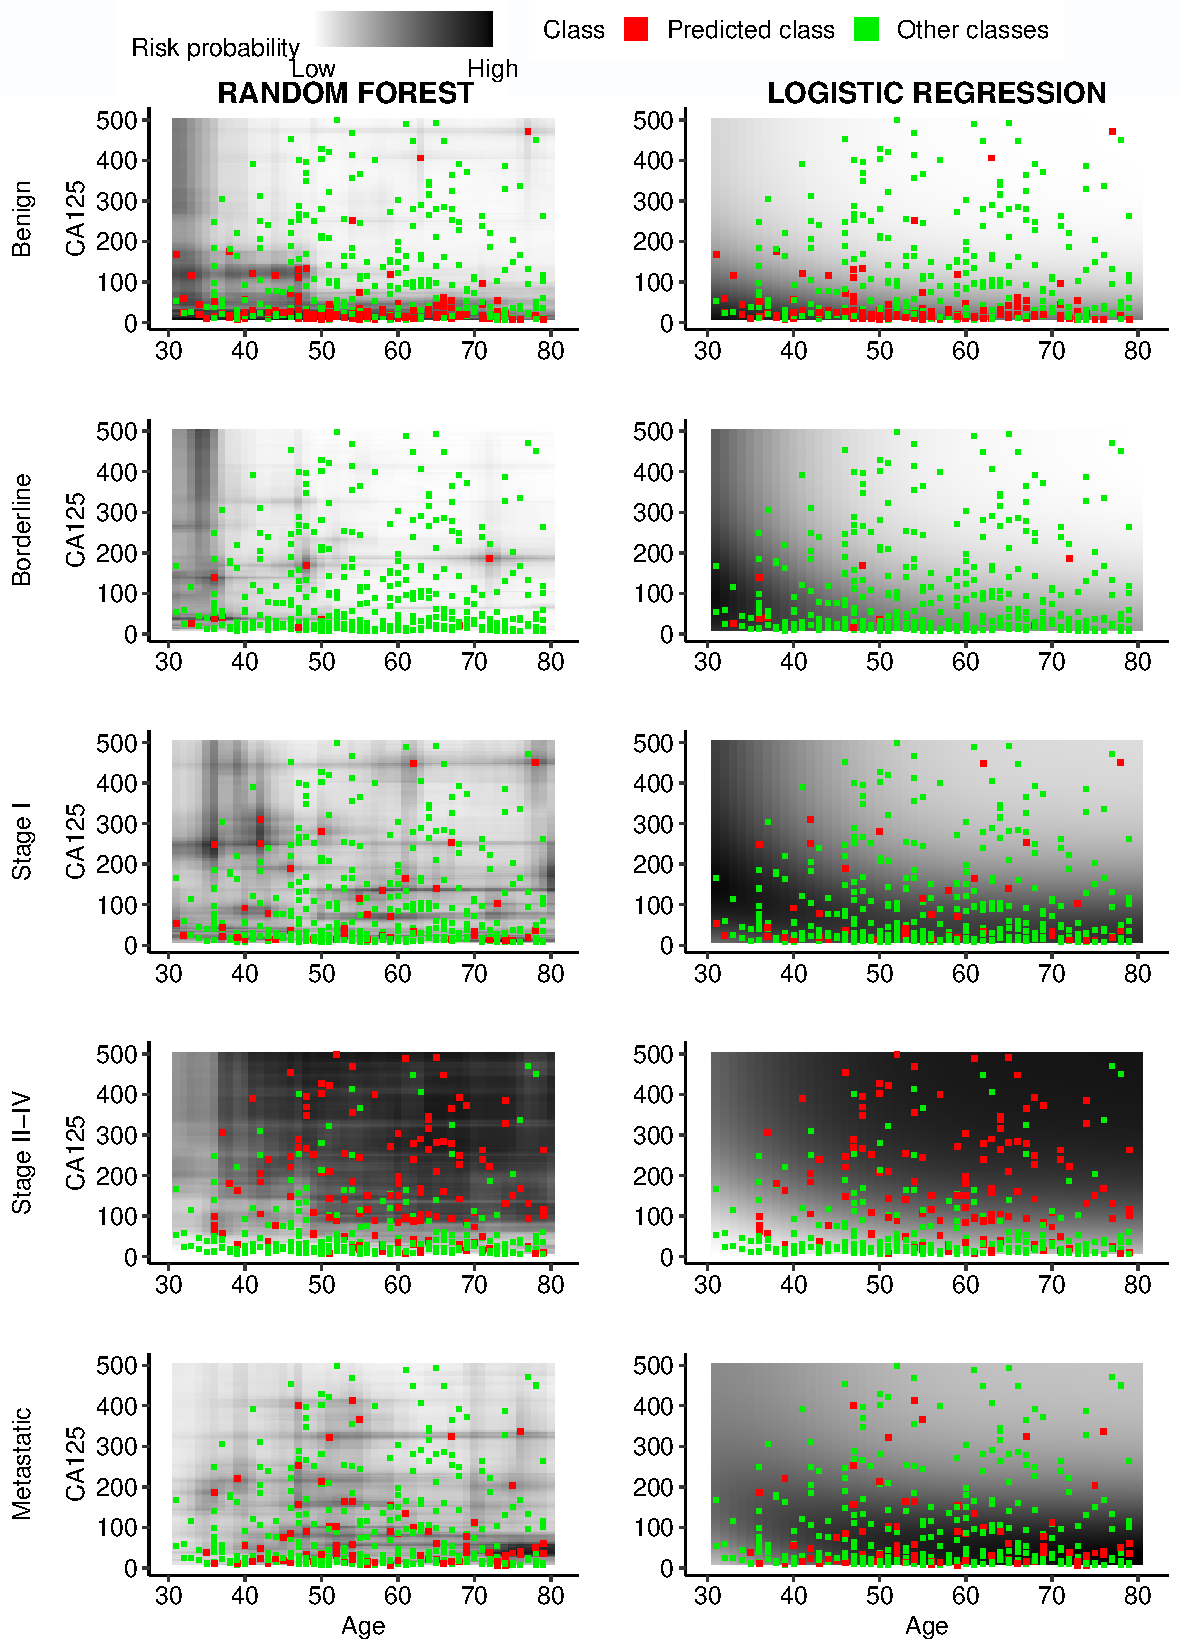
\includegraphics[width=1\textwidth]{figures/RFOverfitting/F1.pdf}
\caption[Heatmap of random forest and logistic regression predictions with training cases]{Random Forest and logistic regression probability estimation in data space for 4 subtypes of ovarian malignancy diagnosis with cases in training set superimposed. CA125 bounded to 500.}
\label{fig:3:1}
\end{figure}

\begin{figure}
\centering
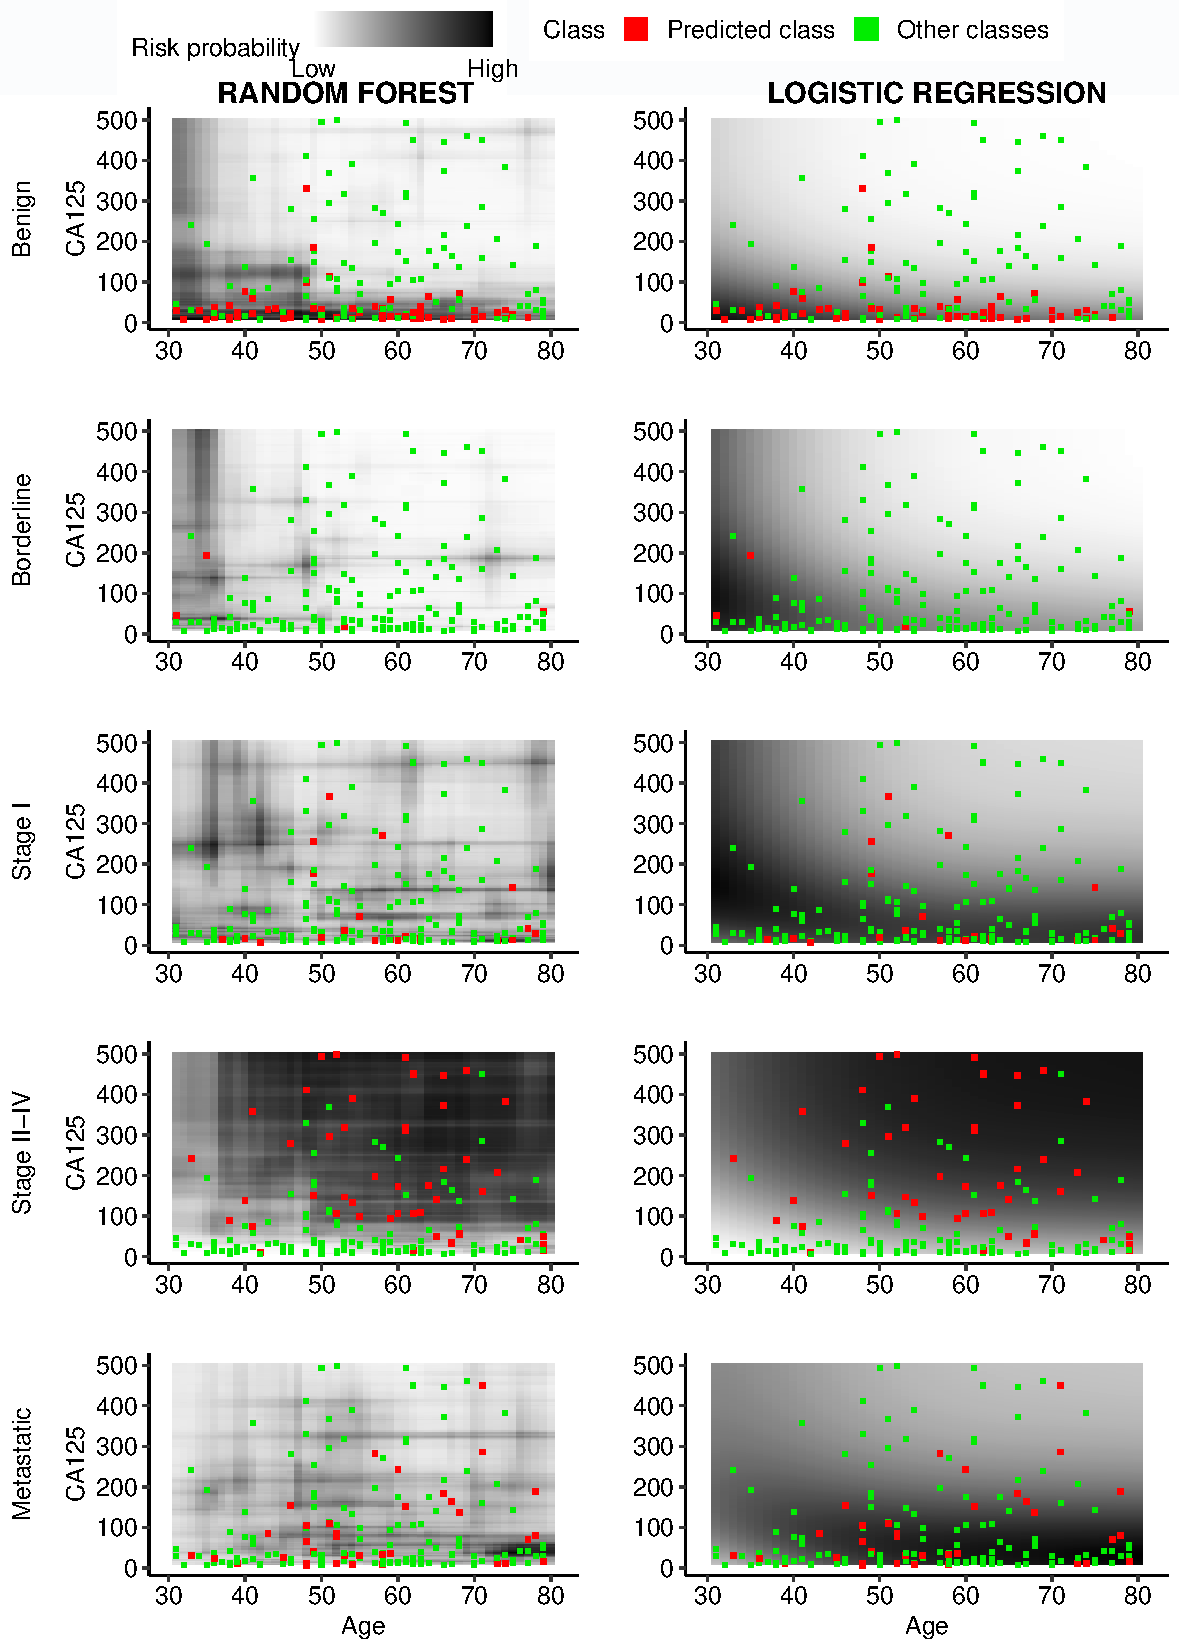
\includegraphics[width=1\textwidth]{figures/RFOverfitting/F2.pdf}
\caption[Heatmap of random forest and logistic regression predictions with test cases]{Random forest and logistic regression probability estimation in data space for 4 subtypes of ovarian malignancy diagnosis with cases in test set superimposed. CA125 bounded to 500.}
\label{fig:3:2}
\end{figure}

\begin{figure}
\centering
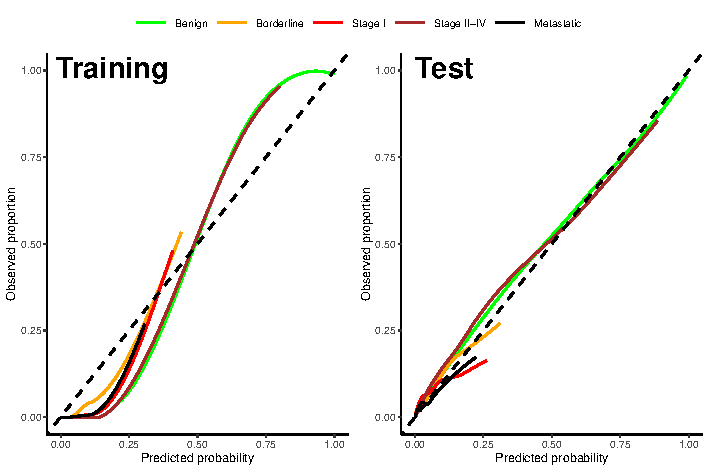
\includegraphics[width=1\textwidth]{figures/RFOverfitting/F3.pdf}
\caption[Calibration plots for random forest model]{Calibration plots for random forest model in ovarian cancer data. Observed proportion is estimated with a LOESS model. The plots only show observed proportions for predicted probabilities between quantiles 5th and 95th.}
\label{fig:3:3}
\end{figure}

\subsection{CRASH3: traumatic brain injury prognosis}
\gls{CRASH}-3 data was collected between 2012 and 2019 for a multicenter, randomized,
placebo-controlled trial to measure the effects of tranexamic acid on death,
disability, vascular occlusive events, and other morbidities in 12,660 patients
with acute traumatic brain injury (\gls{TBI})
 \cite{collaboratorsEffectsTranexamicAcid2019}. We used age (years) and systolic
blood pressure (mmHg) as continuous variables and sex, Glasgow Coma Scale (\gls{GCS})
eye-opening (4 levels), and pupillary reaction (4 levels) as categorical
variables. We performed a complete case analysis (\gls{CCA}) removing patients for
which one or more values were missing obtaining a complete dataset of 12,548
patients. \gls{CCA} was used for simplicity and because the phenomenon under study
should not be affected importantly by this. The outcome was measured 28 days
after randomization: alive ($n = 10{,}022$, 80\%), death due to head injury ($n
= 2309$, 18\%), or death of other cause ($n = 217$, 2\%) (detailed information
in Table S3). The training set included 8783 patients (70\%), and the test set
was 3765 (30\%).

For \gls{RF}, the \gls{PDI} was 0.96 in train data and 0.54 in test data. For \gls{MLR}, the \gls{PDI}
was 0.61 and 0.60, respectively. The heatmaps drew a similar picture compared
with the previous case study: \gls{RF} had clear probability peaks whilst \gls{MLR} had
smoothly changing probabilities (Figures S5--S8). The calibration plots for \gls{RF}
were also similar: poor calibration in training data but decent in the test data
for the 2 most common outcomes (Figure S9).

\subsection{IST: type of stroke diagnosis}
The International Stroke Trial (\gls{IST}) database was designed with the aim of
establishing whether early administration of aspirin, heparin, or both or
neither influenced the clinical course of acute ischaemic stroke
 \cite{sandercockInternationalStrokeTrial2011}. Data for the 19,435 patients with
suspected acute ischaemic stroke were recruited between 1992 and 1996. We use
age (years) and systolic blood pressure (mmHg) as continuous variables, and
conscious state (fully alert vs drowsy), deficit of face (yes vs no), deficit of
arm/hand (yes vs no), deficit of leg/foot (yes vs no), dysphasia (yes vs no),
and hemianopia (yes vs no) as categorical variables. We again performed a \gls{CCA}
retaining 15,141 patients. The outcome is the type of stroke: ischaemic ($n =
13{,}622$, 90\%), indeterminate ($n = 736$, 5\%), hemorrhagic ($n = 439$, 3\%),
or no stroke ($n = 344$, 2\%) (detailed information in Table S4). The training
set included 10,598 patients (70\%), and the test set 4543 (30\%).

The \gls{RF} model had a training \gls{PDI} of 0.89 and a test \gls{PDI} of 0.35. For \gls{MLR}, the
training set \gls{PDI} was 0.39, the test set \gls{PDI} was 0.41. In this dataspace, the
phenomenon is notorious, with very local peaks around train cases
(Figures S10-S13). The calibration plots for training and test data showed poor
calibration (Figure S14).

\section{Simulation study}
\label{sec:3.4}

\subsection{Aim}
We conducted a simulation study to assess which key factors of the modeling
setup (dataset and minimum node size) contribute to the phenomenon of having an
exaggerated \gls{AUC} in the training data without strong signs of overfitting in test
data. We report the simulation study using the \gls{ADEMP} (aims, data-generating
mechanisms, estimands, methods, and performance measures) structure
 \cite{morrisUsingSimulationStudies2019}. The code for the simulation study can
be found in the \gls{OSF} repository (\url{https://osf.io/y5tqv/}).

\subsection{Data-generating mechanism (DGM)}
For the simulation study, we generated data by assuming that the true model was
in the form of an \gls{MLR} with an outcome event fraction of 0.2 (see Additional
file 1: Appendix 1: Simulation Algorithm for details).

The 48 \glspl{DGM} differed according to the following parameters:
\begin{enumerate}[label=(\roman*)]
\item \textit{Predictor distribution}: predictors were either all continuous
with multivariate normal distribution or all binary with 50\% prevalence.
\item \textit{Number of predictors}: there were either 4 true predictors (0
noise predictors), 16 true predictors (0 noise predictors), or 16 predictors of
which 12 noise predictors. Noise predictors had a true regression coefficient
of~0.
\item \textit{Correlation between predictors}: Pearson correlations between all
predictors were either 0 or 0.4.
\item \textit{True AUC}: this was either 0.75 or 0.90.
\item \textit{Balance of regression coefficients}: the true model coefficients
that were not 0 were either all the same (balanced) or not (imbalanced). When
imbalanced, one-fourth of the predictors have a coefficient that is 4 times
larger than the others.
\end{enumerate}

The true model coefficients for generating the data were obtained by trial error
and are available in Table S5.

\subsection{Estimands}
For both training and test data, we estimate model discrimination, whether risk
estimates have too high (overconfidence) or too low (underconfidence) spread and
the prediction error. Underconfidence reflects the situation in Figure \ref{fig:3:3}
(Train): high probabilities are underestimated, and low probabilities are
overestimated. Overconfidence is the opposite: high probabilities are
overestimated, and low probabilities are underestimated. For test data, we also
calculate discrimination loss vs the true model and the relative contribution of
bias and variance to the prediction error. As the training and test samples are
based on the same \gls{DGM}, the test results reflect internal rather than external
validation.

\subsection{Methods}
We fitted models on training datasets of size 200 (small) or 4000 (large), and
for \gls{RF} models we used values for \textit{min.node.size} of 2 or 20 and ranger
package for training. As a result, there were $2 \times 2 \times 3 \times 2
\times 2 \times 2 \times 2 = 192$ scenarios. For each scenario, 1000 simulation
runs were performed (i.e., 1000 different training datasets). For \gls{RF},
\textit{ntree} was fixed at 500, and \textit{mtry} at the square root of the
number of predictors (default value). Models were validated on a single large
test dataset per \gls{DGM} ($N = 100{,}000$) to avoid sampling variability.

\subsection{Performance}
For discrimination we calculated the \gls{AUC} and for confidence of risk estimates
the calibration slope (slope $< 1$ means overconfidence, slope $> 1$
underconfidence). The calibration slope is calculated as the slope of a logistic
regression (\gls{LR}) model fitting the outcome to the logit of the estimated
probabilities as the only predictor. Calibration intercept is calculated fitting
the same model for a slope of 1 by setting the predicted probabilities as an
offset term. Discrimination loss was calculated as the difference between true
\gls{AUC} and median test \gls{AUC}. Finally, the mean squared error (\gls{MSE}) of the predicted
probabilities was calculated according to \cite{friedmanBiasVariance02004} as
the sum of squared bias and variance (see Additional file 1: Appendix 2:
Simulation metrics for details).

\section{Results}

The aggregated simulation results using median and interquartile range for
discrimination and calibration and mean and standard deviation for mean squared
error are available in Additional file 1 (Table S6). The complete simulation
including the code and 1000 simulations for each of the 192 scenarios is
available in the \gls{OSF} repository \cite{barrenadaUnderstandingOverfittingRandom2023}.

\subsection{Discrimination}
In the simulation study, the median training \glspl{AUC} were close to 1 in most of
the cases. The median training \gls{AUC} was between 0.97 and 1 unless there were 4
binary predictors, or 16 binary predictors combined with a minimum node size of
20 (Figure \ref{fig:3:4}). Higher \textit{min.node.size} resulted in less extreme training
\glspl{AUC}.

\begin{figure}
\centering
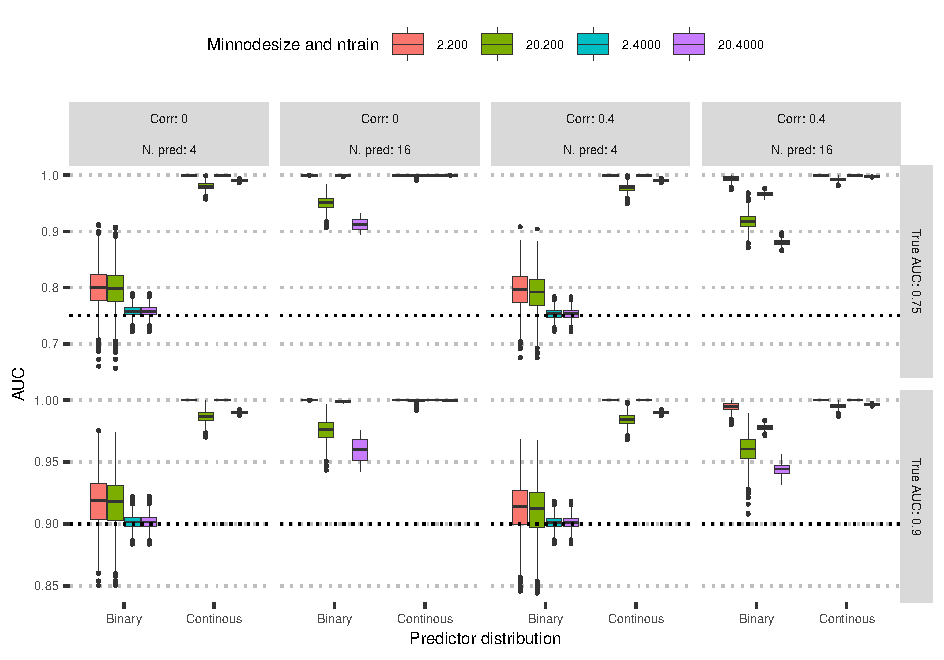
\includegraphics[width=1\textwidth]{figures/RFOverfitting/F4.pdf}
\caption[Simulation training AUC]{Training AUC by simulation factors and modeling hyperparameters in scenarios without noise. Scenarios are aggregated by strength because this simulation factor had minimal effect.}
\label{fig:3:4}
\end{figure}

In general, median test \glspl{AUC} were higher when there was a large vs small
training dataset, high vs low \textit{min.node.size}, high vs low correlation
between predictors, binary versus continuous predictors, and 4 versus 16
predictors (except with correlated continuous predictors) (Figure \ref{fig:3:5}). All other
simulation factors being equal, the scenarios with 4 true and 12 noise
predictors had results for the \gls{AUC} that was identical to scenarios with 16
predictors (Figures \ref{fig:3:4} and \ref{fig:3:5} and S15-16).

\begin{figure}
\centering
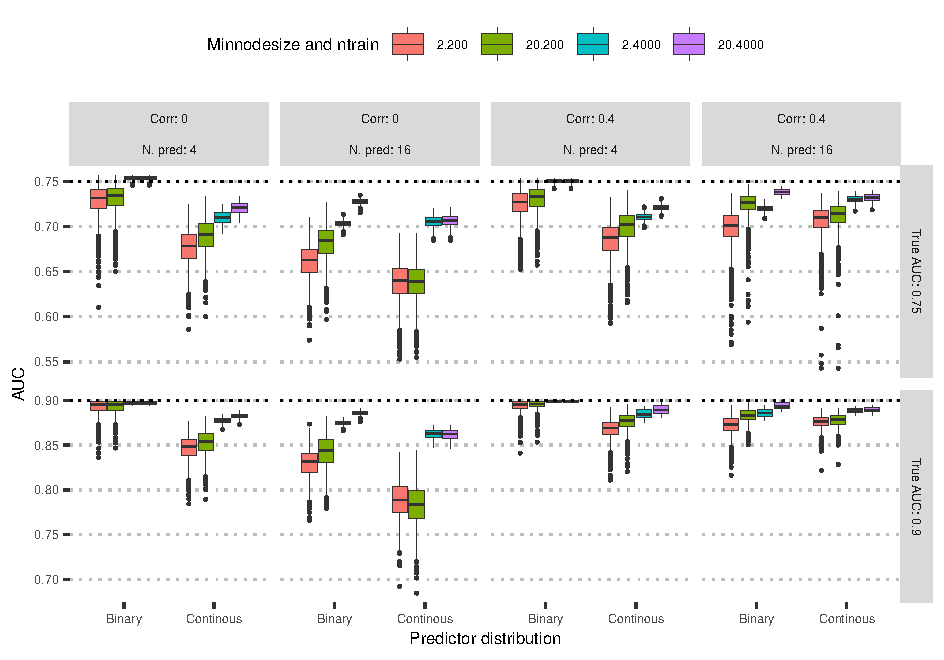
\includegraphics[width=1\textwidth]{figures/RFOverfitting/F5.pdf}
\caption[Simulation test AUC]{Test AUC by simulation factors and modeling hyperparameters in scenarios without noise. Scenarios are aggregated by strength.}
\label{fig:3:5}
\end{figure}

The Spearman correlation between median training \gls{AUC} and discrimination loss was
0.72 for scenarios with a true \gls{AUC} of 0.9, and 0.69 for scenarios with a true
\gls{AUC} of 0.75 (Figure S17). The median discrimination loss was 0.025 (range 0.00
to 0.13). In the 114 scenarios where the median training \gls{AUC} was $\geq 0.99$,
the median discrimination loss was 0.036 (range 0.003 to 0.13). In the other
scenarios, the median discrimination loss was 0.013 (0.00 to 0.069).

\subsection{Calibration}
Median training calibration slopes ranged between 1.10 and 19.4 (Figure \ref{fig:3:6} and
Figure S18): the probability estimates were always underconfident where high
probabilities were underestimated and low probabilities overestimated. This is
the consequence of perfect separation between events and non-events in training
data (i.e., \gls{AUC} $= 1$) which means that any estimation above 0 or below 1 is
underconfident (Figure S19). The median slope was lowest in scenarios with few
binary predictors or higher \textit{min.node.size}. Median test calibration
slopes ranged between 0.45 and 2.34. Across all scenarios, the Spearman
correlation between the median training slope and median test slope was $-0.11$
(Figure S17). Median test slopes were mainly higher when the true \gls{AUC} or
\textit{min.node.size} was higher. In addition, median test slopes tended to be
higher with binary predictors, uncorrelated predictors, and higher sample sizes
(Figure \ref{fig:3:7} and Figure S18). Calibration slopes were similar in scenarios with 16
true predictors, 4 true predictors, and 12 noise predictors (Figures \ref{fig:3:6} and \ref{fig:3:7}
and Figures S20-21). In the 78 scenarios without perfect training (\gls{AUC} $<
0.99$) the median test calibration slope was between 0.59 and 2.34 with a
median of 1.10. In the 114 scenarios with almost perfect training \gls{AUC} ($\geq
0.99$), the median calibration slope was 0.92.

\begin{figure}
\centering
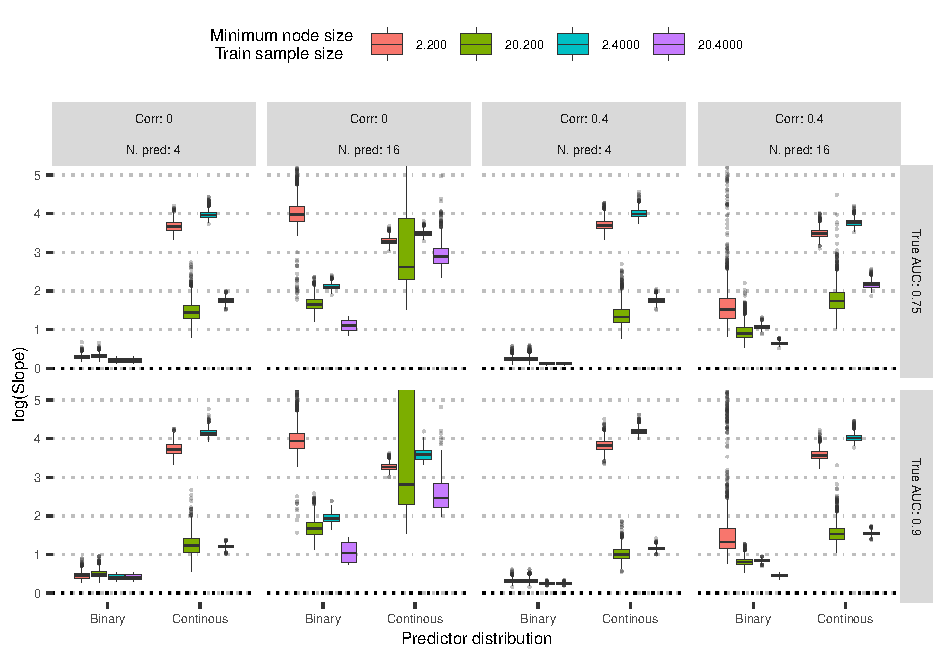
\includegraphics[width=1\textwidth]{figures/RFOverfitting/F6.pdf}
\caption[Simulation training calibration log slope]{Training set calibration log slope by simulation factors and modeling hyperparameters in scenarios without noise. Scenarios are aggregated by strength. The ideal value for the log slope is 0.}
\label{fig:3:6}
\end{figure}

\begin{figure}
\centering
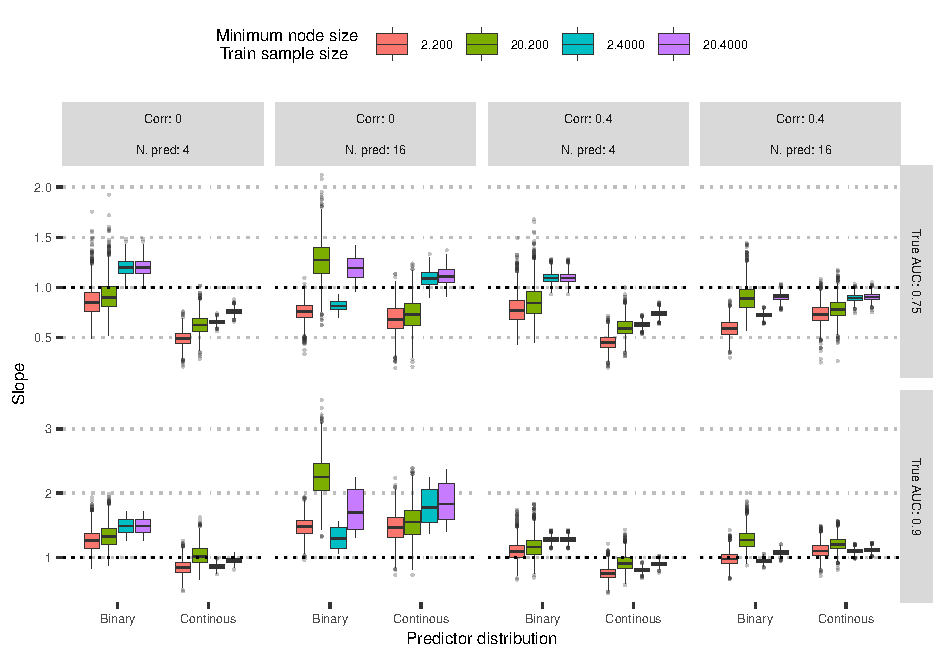
\includegraphics[width=1\textwidth]{figures/RFOverfitting/F7.pdf}
\caption[Simulation test calibration slope]{Test set calibration slope by simulation factors and modeling hyperparameters in scenarios without noise. Scenarios are aggregated by strength. The ideal value for the slope is 1.}
\label{fig:3:7}
\end{figure}

\subsection{Mean squared error (MSE)}
Median \gls{MSE} across scenarios was 0.008 (range 0.000--0.045) with a median
squared bias of 0.002 (range 0.000--0.038) and median variance of 0.005 (range
0.000--0.017). For the 114 scenarios with median training \gls{AUC} $\geq 0.99$, we
observed a median test \gls{MSE} of 0.010 with a median squared bias of 0.004 (range
0.0004--0.0384) and a median variance of 0.006 (range 0.001--0.017). For the
rest of the scenarios, the median test \gls{MSE} was 0.006. Across all scenarios, the
Spearman correlation of mean test squared bias and mean test variance with
median training \gls{AUC} were 0.47 and 0.43, respectively. The correlation with the
discrimination loss was 0.51 for the squared bias and 0.70 for the variance.
Lower sample size in training was associated with higher median test variance,
and with higher median test squared bias in scenarios with continuous predictors.
Lower \textit{min.node.size} (i.e., deeper trees) was associated with a lower
variance but higher bias in test data when the training sample size was small.
More predictors were associated with higher bias, whereas the correlation
between predictors and higher true \gls{AUC} was associated with lower bias
(Figure \ref{fig:3:8}). The models with noise predictors had lower variance and higher bias
compared to scenarios with 4 true and no noise predictors (Figure S22).

\begin{figure}
\centering
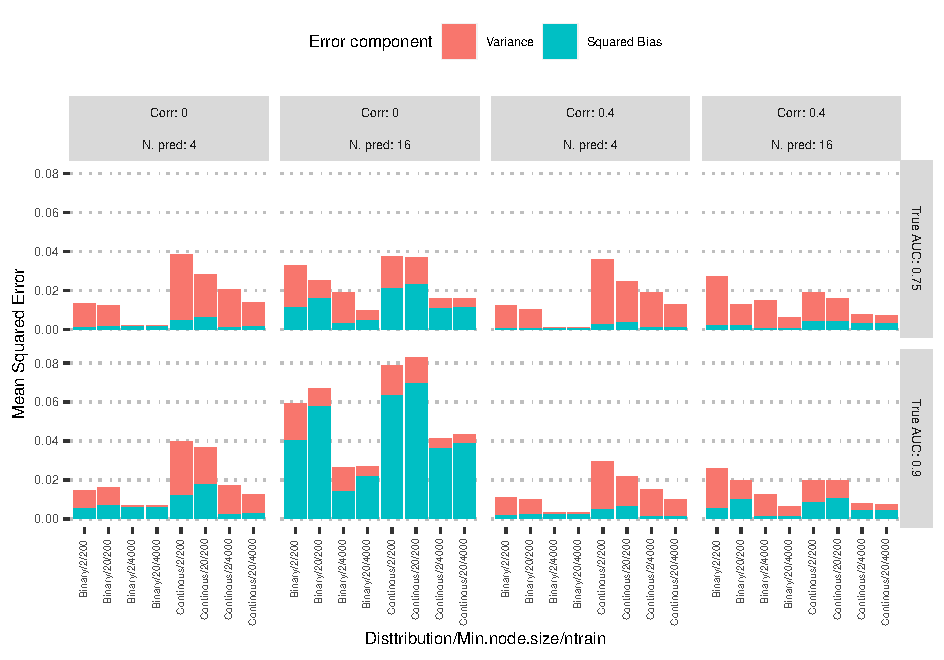
\includegraphics[width=1\textwidth]{figures/RFOverfitting/F8.pdf}
\caption[Simulation mean squared error]{Mean squared error across scenarios without noise aggregated by strength.}
\label{fig:3:8}
\end{figure}

\section{Overall discussion}
\label{sec:3.5}

We tried to better understand and visualize the behavior of random forests for
probability estimation. We make three key observations from this work. First, \gls{RF}
models learn local probability peaks around training set events, in particular
when the trees are very deep (i.e., low \textit{min.node.size}) and when there
are continuous predictors. Where a group of events is located close to one
another in ``data space'', the probability peaks are combined into a region of
increased probability. Where events are isolated in data space, the probability
peaks are very local. Learning through peaks leads to very optimistic (often
near perfect) discrimination in training data, but also to reduced
discrimination in new data compared to models that rely on less deep trees (cf.\
simulation settings where \gls{RF} models with \textit{min.node.size} 2 vs 20 were
fitted on a set of continuous predictors). Probably, the reduction in
discrimination on new data is modest because the local peaks for isolated events
are often harmless for new data: it is unlikely to see an event in the exact
same location. Second, \gls{RF} also suffers from ``classical overfitting'' in which
models with higher discrimination on training data tend to have lower
discrimination on new data than models with less optimistic discrimination (cf.\
simulation settings where \gls{RF} models are learned on 4 binary predictors using 200
vs 4000 training cases). Third, in training and test data, calibration
performance for \gls{RF} models is different from what we commonly observe for \gls{LR}
models. Whereas \gls{LR} based on maximum likelihood leads by definition to
calibration slopes of 1 on training data, calibration slopes for \gls{RF} models were
always above 1 on training data. Also, as opposed to \gls{LR}, calibration slopes for
\gls{RF} models do not converge to 1 on new data. This different behavior is probably
caused by the pragmatic way in which probabilities are obtained for \gls{RF} models,
whilst \gls{LR} estimates probabilities in a principled way through maximum
likelihood.

The simulation results regarding discrimination and calibration go against
fitting very deep trees when using \gls{RF} for probability estimation. This is in
line with recent work that illustrated that \gls{RF} using deeply grown trees results
in risk estimates that are particularly unstable
 \cite{rileyStabilityClinicalPrediction2023}. The heatmaps for our case studies
illustrate how \gls{RF} models with deeply grown trees lead to probabilities that
change non-smoothly with changes in the values of predictors. It has been
suggested to set \textit{min.node.size} to 5\% or 10\% of the sample size
 \cite{malleyProbabilityMachinesConsistent2012,kruppaConsumerCreditRisk2013}.
Alternatively, \textit{min.node.size} can be tuned. Although this was not the
focus of our study, it seems natural to tune with logloss (also known as the
negative loglikelihood or cross-entropy) or Brier score as the loss function
since they capture calibration
 \cite{probstHyperparametersTuningStrategies2019}. In their work, Ledger and
colleagues tuned \textit{min.node.size} by optimizing logloss based on tenfold
cross-validation for 30 random values for mtry and \textit{min.node.size} using
the trainControl and train functions from the caret R package
 \cite{ledgerMulticlassRiskModels2023}. This resulted in $\textit{mtry} = 3$ and
$\textit{min.node.size} = 15$, with competitive results in test data. Applying
the tuneRanger R package with 200 iterations for our case studies based on
logloss yielded an optimal \textit{min.node.size} of 8 (0.1\% of training set
size) for ovarian cancer data, 261 (2.1\%) for \gls{CRASH}3 data and 591 (3.9\%) for
\gls{IST} data \cite{probstHyperparametersTuningStrategies2019}. These values are
higher than the default values in many statistical software programs.

Three comments regarding the interpretation of discrimination and calibration
results for \gls{RF} models are worth making. First, it is well known that apparent
performance, i.e., performance assessment on the exact same dataset that was
used to train the model, is overly optimistic
 \cite{altmanWhatWeMean2000,moonsPROBASTToolAssess2019}. Our work indicates that
this is a fortiori case for \gls{RF}. Unfortunately, some studies present their \gls{RF}
models with ``excellent'' performance because they only present discrimination
for the training data
 \cite{daiUsingRandomForest2018,chenPredictionMalignantMiddle2015,yuanDevelopmentHeartFailure2019}.
Instead, proper internal and external validation results should be reported.
Second, from a regression modeling perspective, a calibration slope that is
clearly below 1 on internal validation is a symptom of overfitting. This cannot
be applied in the same way for \gls{RF} models. Models based on larger training
samples had higher calibration slopes in our simulation study, but a calibration
slope of 1 does not appear to have a special meaning. Models with a calibration
slope above 1 on test data when trained on 200 training samples, had an even
higher slope when trained on 4000 samples. The interpretation of risk estimates
based on \gls{RF} requires caution, probably because probabilities are generated in a
very ad hoc way. Of course, the calibration slope still quantifies in a
descriptive manner whether the risk estimates are on average too confident
(slope $< 1$), not confident enough (slope $> 1$), or fine (slope $= 1$).
Third, despite that \gls{RF} models had high discrimination results in the training
data (suggestive of overfitting), the calibration slope in the training data was
always above 1 (risk estimates show too little spread, suggestive of
underfitting). This appears to be a consequence of the bootstrapping procedure
in combination with the low \textit{min.node.size}. Due to the bootstrapping, a
training set case was part of approximately 63\% of bootstrap samples and
therefore was used for 63\% of the trees in the forest. When averaging the
proportion of events in the appropriate leaf nodes over all \textit{ntree} trees
to get a probability estimate for a given training set case, 63\% of these
proportions are near perfect: close to 1 if the training case is an event,
close to 0 if the training cases is a non-event. The remaining 37\% are more
variable and often far less good. The 63\% near-perfect proportions cause
discrimination to be very high because most events will end up with an estimated
probability of an event that is higher than that for most non-events. The
remaining 37\% of the proportions pull the probability estimates away from 0 (if
the case is a non-event) or 1 (if the case is an event), leading to calibration
slopes $> 1$.

Although the aim of our paper was largely educational, it links to previous more
fundamental work and fills a gap in the literature by explicitly studying
factors that contribute to better discrimination and calibration of new data.
Wyner and colleagues (2017) argued that \gls{RF} has excellent performance because it
is an ``interpolating classifier'', i.e., it is fitted with little to no error
to the train data \cite{wynerExplainingSuccessAdaBoost2017a}. They argue that
the interpolation should not be confused with overfitting. Even if the
individual trees are overfitting, each training set case is not used in about
37\% of the individual trees, such that averaging over trees partially solves
overfitting. Belkin and colleagues have linked this to a double descent curve
for highly flexible algorithms: when the complexity of the model increases, test
set performance first improves, then deteriorates, and finally improves again
once the ``interpolation threshold'' (where perfect training performance is
achieved) is exceeded \cite{belkinFitFearRemarkable2021}. Recently, however,
Buschjäger and Morik opposed the existence of double descent in \gls{RF}
 \cite{buschjagerThereNoDoubleDescent2021}. Mentch and Zhou linked the success of
\gls{RF} to the signal-to-noise ratio (\gls{SNR}) of the data. In their work, they present
that the randomness of \gls{RF} is beneficial in situations with low \gls{SNR} whereas
bagging is preferred if \gls{SNR} is high
 \cite{mentchRandomizationRegularizationDegrees2020}. They explain the success of
\gls{RF} by the low \gls{SNR} of many real-world datasets. This view contradicts the view
that flexible algorithms work best when the \gls{SNR} is high
 \cite{vancalsterMachineLearningMedicine2019}. Finally, the issue of calibration
of estimated probabilities in the context of \gls{RF} models received little attention
in the literature, although it is key for optimal clinical decision making
 \cite{vancalsterCalibrationRiskPrediction2015}. It has been suggested that using
fully grown trees in \gls{RF} leads to suboptimal risk estimates
 \cite{malleyProbabilityMachinesConsistent2012,kruppaConsumerCreditRisk2013}.
However, this is rarely mentioned and hence it is common to see that low minimum
node sizes are recommended because the problem is treated as a classification
problem instead of a probability estimation problem (e.g., see default for
randomForest package or scikit-learn). We think that the current study sheds
further light on probability estimation in \gls{RF}. Of course, a generic alternative
that works for any miscalibrated model is to recalibrate the probabilities of
the \gls{RF} afterward using new data
 \cite{ojedaCalibratingMachineLearning2023}.

We identified the following limitations of our study. Firstly, a simulation
study is always limited by the included scenarios. It would be of interest to
include more simulation factors and values per simulation factor (e.g., for
\textit{min.node.size}) in the simulation study or to include scenarios where \gls{RF}
hyperparameters are tuned rather than fixed. Tuning could improve the
calibration of the models
 \cite{probstHyperparametersTuningStrategies2019,kruppaProbabilityEstimationMachine2014a}.
However, the simulation study already had 192 scenarios, and adding more factors
or values would increase the computational cost exponentially and would
overcomplicate the interpretation of the results. Topics that could be
investigated in further simulation studies include varying other hyperparameters
than \textit{min.node.size} (e.g., \textit{mtry}, sampling fraction, splitting
rule) and investigating more values for sample size, number of predictors, the
proportion of noise predictors, and min.node.size. Secondly, we were using
logistic \glspl{DGM} without nonlinear or nonadditive associations with the outcome. We
assumed that the impact of this would be limited, because the focus was not on
the comparison of \gls{RF} with \gls{LR}, and any nonlinearity or nonadditivity (including
the absence of it) has to be learned by the algorithm. Thirdly, the traditional
\gls{RF} algorithm selects variables at each split in a way that favors continuous
over binary variables \cite{stroblBiasRandomForest2007}. Continuous variables
can split in many ways, such that there is often a split that, perhaps by
chance, has a better Gini impurity reduction than the Gini impurity reduction
for a binary variable. The splits for continuous variables may often overfit,
thereby increasing training discrimination but decreasing test discrimination.
It is well documented that this affects variable importance measures
 \cite{stroblBiasRandomForest2007}, but it may also be relevant for model
performance. The problem can be addressed by using an adapted \gls{RF} algorithm such
as cforest from the partykit package
 \cite{hothornUnbiasedRecursivePartitioning2006}. These adapted algorithms grow
conditional inference trees (\gls{CIT}) instead of classification trees. For the case
studies, we observed that tuning and using the adapted \gls{RF} yields a less
optimistic training \gls{AUC} and similar or slightly better test performance (see \gls{OSF}
Repository \cite{barrenadaUnderstandingOverfittingRandom2023}. However, our aim was to understand
how the characteristics of the data and the modeling process affected the
models, hence we did not systematically explore the effects of tuning or
alternative algorithms.

We conclude that \gls{RF} tends to exhibit local overfitting by learning probability
peaks, in particular when the \gls{RF} model is based on deeply grown trees. This
local overfitting can lead to highly optimistic (near perfect) discrimination on
the training data but to reduced discrimination on new data compared to \gls{RF}
models based on less deeply grown trees. In line with the work of Kruppa and
colleagues \cite{kruppaProbabilityEstimationMachine2014a}, our results go
against the recommendation to use fully grown trees when using \gls{RF} for
probability estimation.

\section*{Availability of data and materials}
All data and code that support the findings of this study are openly available
in the \gls{OSF} repository
 \cite{barrenadaUnderstandingOverfittingRandom2023} except the ovarian cancer
dataset which is not publicly available.

\section*{Acknowledgements}
Partial findings from this paper were presented at the Young Statisticians
Meeting 2023 in Leicester (July) and in the Conference of the International
Society of Clinical Biostatistics (ISCB) 2023 in Milan (August).

\section*{Other information}
\subsection*{Funding}
This research was supported by the Research Foundation--Flanders (FWO) under
grant G097322N with BVC and DT as supervisors.

\subsection*{Conflicts of interest}
The authors declare that they have no competing interests.

\subsection*{Contributors}
Contributions were based on the CRediT taxonomy. Conceptualization: LB, BVC.
Funding acquisition: BVC, DT. Project administration: LB. Supervision: BVC.
Methodology: LB, PD, ALB, BVC. Resources: LB, DT, BVC. Investigation: LB, PD,
DT, ALB, BVC. Validation: LB, BVC. Data curation: LB. Software: LB, BVC.
Formal analysis: LB, BVC. Visualization: LB, BVC. Writing---original draft: LB,
BVC. Writing---review and editing: all authors. All authors have read, share
final responsibility for the decision to submit for publication, and agree to be
accountable for all aspects of the work.

\chapter[Clustered calibration plots]{Clustered flexible calibration plots for binary outcomes using random effects modeling}
% Only include if the thesis is written as a collection of papers
%_________________________
\label{sec:chp_ClusteredCalibration}

\glsunset{ADNEX}
\glsunset{AUC}
\glsunset{CGC}
\glsunset{CI}
\glsunset{CPM}
\glsunset{DGM}
\glsunset{EPC}
\glsunset{GLMM}
\glsunset{ICC}
\glsunset{IOTA}
\glsunset{IPD}
\glsunset{MIXC}
\glsunset{MSCE}
\glsunset{OSF}
\glsunset{PI}
\glsunset{TMAC}
\glsunset{TRIPOD}


published as:
\begin{quote}
Barre\~{n}ada L, De Cock Campo B, Wynants L \& Van Calster B. Clustered flexible calibration plots for binary outcomes using random effects modeling. Research Synthesis Methods. 2025;1--22. https://doi.org/10.1017/rsm.2025.10046
\end{quote}
%_________________________

\section*{Abstract}
Evaluation of clinical prediction models across multiple clusters, whether centers or datasets, is becoming increasingly common. A comprehensive evaluation includes an assessment of the agreement between the estimated risks and the observed outcomes, also known as calibration. Calibration is of utmost importance for clinical decision making with prediction models and it may vary between clusters. We present three approaches to take clustering into account when evaluating calibration. (1) Clustered group calibration (\gls{CGC}), (2) two-stage meta-analysis calibration (\gls{TMAC}) and (3) mixed model calibration (\gls{MIXC}) can obtain flexible calibration plots with random effects modelling and providing confidence and prediction intervals. As a case example, we externally validate a model to estimate the risk that an ovarian tumor is malignant in multiple centers (N = 2489). We also conduct a simulation study and synthetic data study generated from a true clustered dataset to evaluate the methods. In the simulation study \gls{MIXC} and \gls{TMAC} (splines) gave estimated curves closest to the true overall curve. In the synthetic data study \gls{MIXC} produced cluster specific curves closest to the truth. Coverage of the prediction interval across the plot was best for \gls{TMAC} with splines. We recommend using \gls{TMAC} with splines to estimate the overall curve and the 95\% \gls{PI} and \gls{MIXC} for the cluster specific curves, especially when sample size per cluster is limited. We provide ready-to-use code to construct summary flexible calibration curves with confidence and prediction intervals to assess heterogeneity in calibration across datasets or centers.

\section{Introduction}
Clinical prediction models (\glspl{CPM}) are evidence-based tools that estimate the probability of health-related events either at the time of evaluation (diagnosis) or at some point in the future (prognosis) \cite{steyerbergClinicalPredictionModels2019a,vansmedenClinicalPredictionModels2021}. These risk estimates play a crucial role in evidence-based decision-making and can be of great value when counselling patients. However, to ensure the reliability of risk estimates, \glspl{CPM} must exhibit good calibration \cite{vancalsterCalibrationHierarchyRisk2016}. Calibration assesses how well the predicted risks correspond to observed risks \cite{vancalsterCalibrationHierarchyRisk2016}. In recent years, there has been a notable increase in studies involving multiple clusters. The term "cluster" can refer to different groupings within the population under study, depending on the context. For example, in multicenter studies, a cluster commonly refers to different centers, whereas in meta-analysis, a cluster may pertain to each study or centers within the study where possible (e.g. individual patient data (\gls{IPD}) meta-analysis \cite{rileyIndividualParticipantData2021a}). In this work, the term "cluster" will specifically denote a center in a multicenter study, but the methods proposed apply more generally as well. An analysis of \glspl{CPM} included in Tufts PACE (Predictive Analytics + Comparative Effectiveness), developed after the year 2000, revealed that 64\% of the models utilized multicenter (clustered) data, indicating a growing trend in such studies \cite{wynantsUntappedPotentialMulticenter2019,wesslerTuftsPACEClinical2017}. \gls{TRIPOD} (Transparent Reporting of a Multivariable Prediction Model for Individual Prognosis or Diagnosis) has addressed this development by publishing an extension known as \gls{TRIPOD}-Cluster \cite{debrayTransparentReportingMultivariable2023}. This extension underscores the importance of taking clustering into account when developing or evaluating prediction models.

Miscalibration can have a harmful influence on medical decision making \cite{vancalsterCalibrationRiskPrediction2015}. It is common to observe heterogeneity in model performance across centers or studies, most notably in model calibration \cite{vancalsterValidationModelsDiagnose2020,guptaDevelopmentValidationISARIC2021,steyerbergAssessmentHeterogeneityIndividual2019,vanAmsterdamCausalViewpoint2024}. It can thus be misleading to generalize performance results from single-cluster data \cite{wynantsDoesIgnoringClustering2018,debrayFrameworkDevelopingImplementing2013,dejongDevelopingMoreGeneralizable2021,moherGuidanceDevelopersHealth2010}. For these reasons, it is crucial to collect clustered data to investigate and quantify heterogeneity in calibration performance between clusters. The presence of clustering introduces challenges, as individuals are no longer independent due to correlations among patients within the same cluster \cite{snijdersMultilevelAnalysisIntroduction2012,finchMultilevelModelingUsing2019a}. Traditional (non-clustered) methodologies should therefore be adapted for use with clustered data.

The most informative assessment of calibration performance for a prediction model is a calibration plot, used to assess whether, among patients with the same estimated risk of the event, the observed proportion of events equals the estimated risk \cite{vancalsterCalibrationHierarchyRisk2016,vancalsterPerformanceEvaluationPredictive2024}.A calibration plot has estimated risks on the x-axis, and the observed proportion on the y-axis. For binary outcomes, observed outcome values are \(Y = 0\) (no event) or \(Y = 1\) (event). The observed proportion of individuals with the event conditional on estimated risk are not observed directly, but are estimated. One approach consists of creating \(Q\) groups (usually based on quantiles of estimated risks) and estimating the observed proportion in each of the groups as the proportion of individuals with the condition. We refer to this approach throughout the text as grouped calibration. The calibration plot then has \(Q\) dots representing the mean risk (value on the x-axis) and observed proportion (value on the y-axis). Another approach is using a flexible model \cite{austinGraphicalAssessmentInternal2014}. The observed outcome is regressed on the estimated probabilities using a smoother such as local regression (loess) or splines. The smoothed relation or \(Q\) groups are plotted together with a line of identity which represents perfect calibration. The grouped approach loses information by categorizing the estimated risks, and depends on the value of \(Q\) and the grouping approach. Flexible models are dependent on smoothing parameters. Flexible calibration curves have been presented for different problems like survival models \cite{austinGraphicalCalibrationCurves2020}, competing risk models \cite{austinGraphicalCalibrationCurves2022}, or multiclass models \cite{vanhoordeSplinebasedToolAssess2015}. Flexible calibration curves that consider clustering have been understudied. Although summarizing statistics of calibration (e.g. O:E) can be meta-analysed across clusters, such summarizing statistics are by definition less informative than the calibration plot \cite{vancalsterPerformanceEvaluationPredictive2024,debrayGuideSystematicReview2017}. We present three different approaches to construct flexible calibration curves from clustered data, provide cluster-specific curves, and quantify heterogeneity using prediction intervals. We illustrate the methodologies with a real case example on ovarian cancer data and compare the performance of the methodology using simulated data, and synthetic data. Section 2 presents the motivating example, the general notation used through the paper, and introduces the three approaches to obtain calibration plots accounting for clustering. Section 3 and 4 present the methodology and results of the simulation study and synthetic data analysis, respectively, and in section 5 we conclude by discussing our findings. This study is an initial assessment of methods for clustered calibration analysis that we classify as a phase 2 methodological study in the four phase framework from Heinze and colleagues \cite{heinzePhasesMethodologicalResearch2024}.

\section{Methods}
\subsection{\texorpdfstring{Motivating example: ADNEX model and Ovarian cancer data}{Motivating example: ADNEX model and Ovarian cancer data}}
The methods will be illustrated using the \gls{ADNEX} model for ovarian tumor discrimination that was developed with data from the International Ovarian Tumor Analysis (\gls{IOTA}) group \cite{vancalsterEvaluatingRiskOvarian2014,timmerman2024}. The \gls{ADNEX} model is a multinomial regression mixed model with random intercepts per center to estimate the probability that an ovarian mass is malignant. Predicting malignancy of ovarian masses prior to surgery is important because benign masses can be managed conservatively, and malignant masses require different surgical approaches depending on the malignant subtype. \gls{ADNEX} estimates the risk of five outcomes: benign tumor, borderline tumor, stage I invasive cancer, stage II-IV invasive cancer, and secondary metastasis. This work will focus on the overall risk of malignancy, which is obtained by adding the risks for the malignant subtypes. \gls{ADNEX} has three clinical and six ultrasound predictors: age, serum CA125 level, type of center (oncology center or other hospital type), maximal diameter of the lesion, proportion of solid tissue, number of papillary projections, presence of \textgreater10 locules, acoustic shadows, and ascites. CA125 is optional, and in this work we focus on \gls{ADNEX} without CA125. \gls{ADNEX} coefficients already capture some of the between-center heterogeneity through the type of center. To illustrate multicenter calibration of the \gls{ADNEX} model we use an external validation dataset of 2489 patients recruited in 17 hospitals \cite{kaijserEvidencebasedApproachDiagnosis2015}. Previous external validation of \gls{ADNEX} on this dataset suggested that there was important heterogeneity between hospitals (Figure S1) \cite{vancalsterValidationModelsDiagnose2020}. To avoid computation errors, three small non-oncology centers in Italy were combined, as well as two small non-oncology centers in the United Kingdom. The dataset then contains 14 clusters, with a median number of 189 patients per cluster (range 38 to 360) (Figure~\ref{fig:4:1}). The mean estimated probabilities (range 0.10 to 0.53) and the prevalence of malignancy (range 0.16 to 0.72) varied between clusters. The intra-cluster correlation (\gls{ICC}) in (logit) malignancy risk based on the null random intercept model is 15\% \cite{snijdersMultilevelAnalysisIntroduction2012}. An \gls{ICC} of 0 would mean that all clusters are similar, and all variance in the logit malignancy risk is due to individual-level variability.

\begin{figure}
\centering
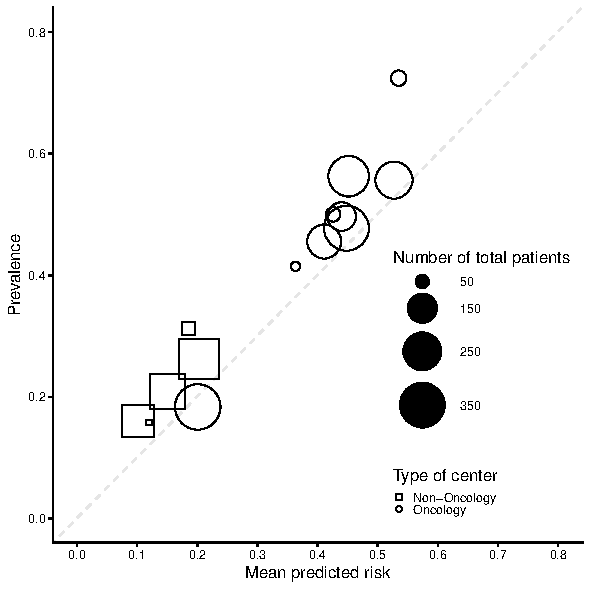
\includegraphics[width=0.8\textwidth]{figures/ClusteredCalibration/F1.pdf}
\caption[Mean predicted risk of ADNEX and prevalence across 14 centers]{Prevalence and mean predicted ADNEX risk by center across the 14 centers in the dataset. The dashed diagonal line indicates perfect calibration.}
\label{fig:4:1}
\end{figure}

\subsection{Notation}
We assume to have a dataset with a total of \emph{J} clusters and use \(j = (1,\ldots,J)\) to index the clusters. In each cluster, we have \(n_{j}\) patients and we index the patients using \(i = \left( 1,\ldots,n_{j} \right)\). The total sample size is \(N = \sum_{j = 1}^{J}n_{j}\)\emph{.} We use \(y_{ij} \in 0,1\) to denote the outcome of patient \(i\) in cluster \(j\), which takes on the value 0 in case of a non-event and 1 in case of an event. We assume that \(y_{ij}\) follows a Bernoulli distribution \(y_{ij} \sim \text{Bern}\left( \pi_{ij} \right)\), where \(\pi_{ij}\) denotes the probability of experiencing the event. Typically, \(\pi_{ij}\) is expressed as a function of a set of risk characteristics, captured in the covariate vector \(\mathbf{x}_{ij}\) and we assume that there exists an unknown regression function \(r\left( \mathbf{x}_{ij} \right) = P\left( y_{ij} = 1 \middle| \mathbf{x}_{ij} \right)\). We approximate this function using a risk prediction model, where we model the outcome as a function of the observed risk characteristics and employ statistical or machine learning techniques to estimate this model. A general expression that encompasses both types is

\begin{equation}{r}
\text{P}\left( y_{ij} = 1\mid\mathbf{x}_{ij} \right) = \pi\left( \mathbf{x}_{ij} \right) = f\left( \mathbf{x}_{ij} \right)\
\label{eq:3:1}
\end{equation}

Where \(f( \cdot )\) denotes the predicted risk given covariate vector \(\mathbf{x}_{ij}\). In a logistic regression model, we have that

\[\pi\left( \mathbf{x}_{ij} \right) = \frac{e^{\mathbf{x}_{ij}^{T}\mathbf{\beta}}}{1 + e^{\mathbf{x}_{ij}^{T}\mathbf{\beta}}}\]

where \(\mathbf{\beta}\) denotes the parameter vector. We can rewrite the above equation to

\[{{\ \ \ \log}\left( \frac{\pi\left( \mathbf{x}_{ij} \right)}{1 - \pi\left( \mathbf{x}_{ij} \right)} \right) = \mathbf{x}_{ij}^{T}\mathbf{\beta}}{\text{logit}\left( \pi\left( \mathbf{x}_{ij} \right) \right)\mathbf{=}\mathbf{x}_{ij}^{T}\mathbf{\beta}}\]

We can employ splines to allow for a non-linear relationship between the covariates and outcome \cite{harrellRegressionModelingStrategies2015}. To estimate equation \ref{eq:3:1}, we fit a statistical or machine learning model to the training data. The resulting model fit then provides us with the predicted probability \(\widehat{\pi}\left( \mathbf{x}_{ij} \right)\).

Using calibration curves, we examine how well the predicted probabilities correspond to the actual event probabilities \cite{steyerbergClinicalPredictionModels2019a,vancalsterCalibrationHierarchyRisk2016,dimitriadisHonestCalibrationAssessment2023,decockcampoReliablePredictiveAnalytics2023}. A calibration plot maps the predicted probabilities \(\widehat{\pi}\left( \mathbf{x}_{ij} \right)\) to the actual event probabilities \(\text{P}\left( y_{ij} = 1\mid\widehat{\pi}\left( \mathbf{x}_{ij} \right) \right)\ \)and hereby provides a visual representation of the alignment between the model's estimated risks and the true probabilities. For a perfectly calibrated model, the calibration curve follows the diagonal as \(\text{P}\left( y_{ij} = 1\mid\widehat{\pi}\left( \mathbf{x}_{ij} \right) \right)\  = \pi\left( \mathbf{x}_{ij} \right)\) for all \(i\).

\subsection{Flexible calibration plots ignoring clustering}
We can estimate the calibration curve using a logistic regression model \cite{decockcampoReliablePredictiveAnalytics2023,onbehalfoftopicgroupevaluatingdiagnostictestsandpredictionmodelsofthestratosinitiativeCalibrationAchillesHeel2019,coxTwoFurtherApplications1958}

\[\text{logit}\left( \text{P}\left( y_{ij} = 1\mid\widehat{\pi}\left( \mathbf{x}_{ij} \right) \right) \right)\mathbf{=}\alpha + \zeta\ \text{logit}\left( \widehat{\pi}\left( \mathbf{x}_{ij} \right) \right)\]

where we estimate the observed proportions as a function of the (logit transformed) predicted probabilities. Using the fitted model, we create a calibration curve by plotting the \(\widehat{\pi}\left( \mathbf{x}_{ij} \right)\) against the observed proportions \(\widehat{P}\left( y_{ij} = 1\mid\widehat{\pi}\left( \mathbf{x}_{ij} \right) \right)\). This model, however, only allows for a linear relationship and, as such, does not adequately capture moderate calibration. To allow for a non-linear relationship between \(\widehat{\pi}\left( \mathbf{x}_{ij} \right)\) and \(y_{ij}\), we can rely on non-parametric smoothers, such as locally estimated scatterplot smoothing (loess) or restricted cubic splines

\[\text{logit}\left( \text{P}\left( y_{ij} = 1\mid\widehat{\pi}\left( \mathbf{x}_{ij} \right) \right) \right)\mathbf{=}s\left( \text{logit}\left( \widehat{\pi}\left( \mathbf{x}_{ij} \right) \right) \right).\]

Here, \(s( \cdot )\) denotes the smooth function applied to the logit transformed predicted probability. This results in a flexible calibration plot, which is implemented in R packages such as CalibrationCurves (val.prob.ci.2 function), rms (val.prob function), or tidyverse (cal\_plot\_logistic function) \cite{vancalsterCalibrationHierarchyRisk2016,harrellRegressionModelingStrategies2015,wickhamWelcomeTidyverse2019,rcoreteamLanguageEnvironmentStatistical2024}.

Figure~\ref{fig:4:2} presents a flexible calibration curve (using a restricted cubic spline) based on the motivating example with pooled data, and the results of a grouped calibration assessment for ovarian malignancy prediction. The panel below shows the sample distribution of the estimated risks for benign cases (blue) and malignant cases (red). The plots suggest that risks were estimated too low.

\begin{figure}
\centering
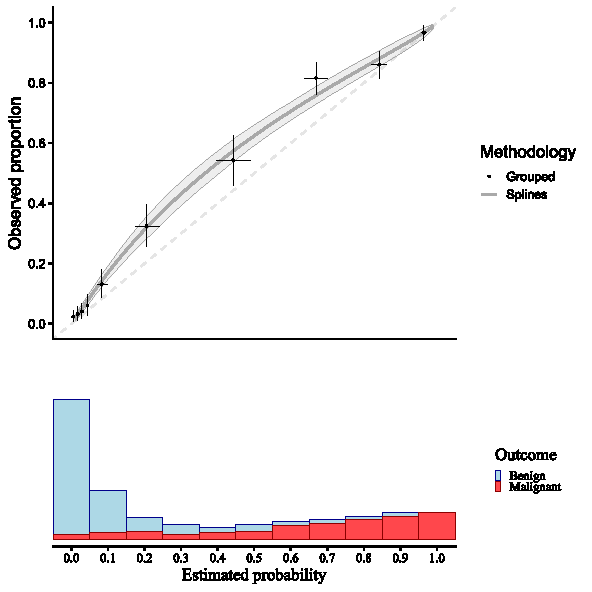
\includegraphics[width=0.8\textwidth]{figures/ClusteredCalibration/F2.pdf}
\caption[Traditional flexible calibration plots and risk distributions]{Traditional flexible calibration curves for the ADNEX model in the motivating example. Observed proportion is estimated with a logistic model with restricted cubic splines to model non-linear effects, and estimated risks are grouped in 10 groups. Confidence intervals are shown for 1000 bootstraps with a shaded area for splines and a + for grouped calibration. The dashed diagonal line indicates perfect calibration.}
\label{fig:4:2}
\end{figure}

Since there is no commonly accepted way to estimate calibration curves for prediction models in clustered data, we present three approaches covering different statistical methodologies. First, we present a grouped clustered calibration plot based on a bivariate random effects meta-analysis model (Clustered Group Calibration; \gls{CGC}). Second, we introduce a two-stage univariate random effects meta-analytical approach for the estimation of the observed events (Two-stage meta-analysis calibration; \gls{TMAC}). Finally, we provide a one-step approach where we fit a random effects model with smooth effects to obtain individual calibration slopes per cluster (Mixed model calibration; \gls{MIXC}). We present the summary of the three proposed approaches in Table~\ref{tab:4:1}.

\begin{table}
\centering
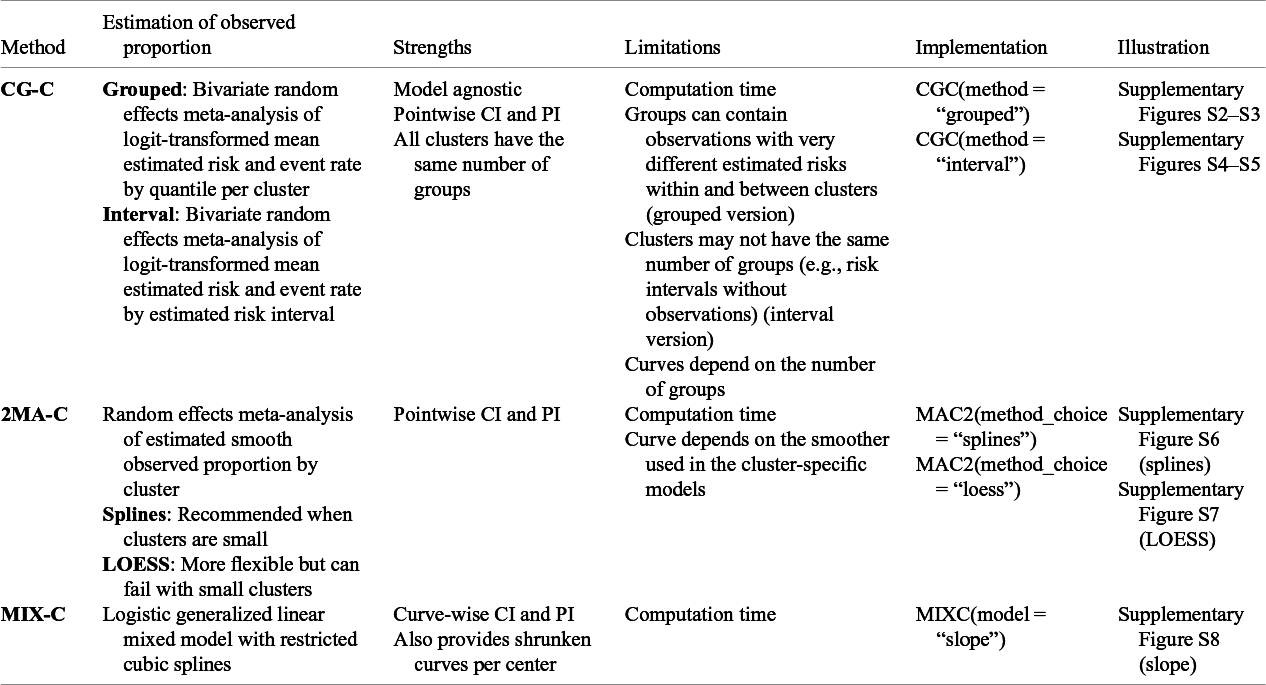
\includegraphics[width=1\textwidth]{figures/ClusteredCalibration/T1.png}
\caption[Overview introduced methods]{Overview of introduced methodologies for creating flexible calibration curves accounting for clustering.}
\label{tab:4:1}
\end{table}

\subsection{Clustered group calibration (CG-C)}
The \gls{CGC} approach is a two-stage approach that extends the traditional grouped calibration approach to clustered data. In the traditional approach, data is pooled and groups are created based on quantiles (often deciles). In \gls{CGC}, we create \(Q\) quantiles in every cluster (based on the estimated risk distribution per cluster) with \(q = (1,\ldots,Q)\). Hereafter, we pool the estimated risks and observed proportions with a bivariate random effects meta-analysis at each quantile \(q\). The logit-transformed observed proportion and average estimated risk are the response variables and we capture the cluster-specific deviation by including a random intercept. The equation of this model is given by

\begin{equation}{r}
\genfrac{[}{]}{0pt}{}{\text{logit(}{\overline{y}}_{qj})}{\text{logit(}{\overline{\widehat{\pi}}}_{qj})} = \genfrac{[}{]}{0pt}{}{{{}_{\overline{y}}\mu}_{q} + u_{qj} + \varepsilon_{qj}}{{_{\overline{\widehat{\pi}}}^{}\mu}_{q} + \nu_{qj} + \epsilon_{qj}}
\end{equation}

where \({\overline{y}}_{qj}\) denotes the prevalence of cluster \(j\) within quantile \(q\) and \({\overline{\widehat{\pi}}}_{qj}\) the average estimated risk in cluster \(j\) within quantile \(q\). We use the subscript \(q\) in the quantities to indicate that this refers to quantile \(q\). \(u_{qj}\) and \(\nu_{qj}\) represent the random intercepts for cluster \(j\), capturing the between-cluster heterogeneity whereas \(\varepsilon_{qj}\) and \(\epsilon_{qj}\) account for the within-cluster error. In this model, we assume that \({{}_{\overline{y}}\mu}_{q} + u_{qj}\) and \({_{\overline{\widehat{\pi}}}^{}\mu}_{q} + \nu_{qj}\) are randomly drawn from a distribution with mean (or pooled) \({{}_{\overline{y}}\mu}_{q}\) and \({_{\overline{\widehat{\pi}}}^{}\mu}_{q}\), respectively. Additionally, we assume that

\[\begin{bmatrix}
u_{qj} \\
\nu_{qj}
\end{bmatrix} \sim \mathcal{N}\left( \genfrac{[}{]}{0pt}{}{0}{0},\Omega_{q} \right)\ and\ \begin{bmatrix}
\varepsilon_{qj} \\
\epsilon_{qj}
\end{bmatrix} \sim \mathcal{N}\left( \genfrac{[}{]}{0pt}{}{0}{0},\Sigma_{qj} \right)\]

where \(\Omega_{q}\) and \(\Sigma_{qj}\) represent the between-cluster and within-cluster covariance matrices within quantile \emph{q}, respectively.

\[\Omega_{q} = \begin{bmatrix}
{}_{\overline{y}}\tau_{q}^{2} & {}_{b}\rho_{q} \; {}_{\overline{y}}\tau_{q} \; {}_{\overline{\widehat{\pi}}}\tau_{q} \\
{}_{b}\rho_{q} \; {}_{\overline{y}}\tau_{q} \; {}_{\overline{\widehat{\pi}}}\tau_{q} & {}_{\overline{\widehat{\pi}}}\tau_{q}^{2}
\end{bmatrix}\]

\[\Sigma_{qj} = \begin{bmatrix}
{}_{\overline{y}}\sigma_{qj}^{2} & {}_{w}\rho_{q} \; {}_{\overline{y}}\sigma_{qj} \; {}_{\overline{\widehat{\pi}}}\sigma_{qj} \\
{}_{w}\rho_{q} \; {}_{\overline{y}}\sigma_{qj} \; {}_{\overline{\widehat{\pi}}}\sigma_{qj} & {}_{\overline{\widehat{\pi}}}\sigma_{qj}^{2}
\end{bmatrix}\]

We use \({}_{\overline{y}}\sigma_{qj}^{2}\) and \({}_{\overline{\widehat{\pi}}}\sigma_{qj}^{2}\) to denote the variance of \({\overline{y}}_{qj}\) and \({\overline{\widehat{\pi}}}_{qj}\), \({}_{w}\rho_{q}\) represents the within-cluster correlation and \({}_{b}\rho_{q}\) the between-cluster correlation in quantile \emph{q}. The between-study variance is denoted as \({}_{\overline{y}}\tau_{q}^{2}\) and \({}_{\overline{\widehat{\pi}}}\tau_{q}^{2}\). For each quantile \emph{q,} we use a bivariate meta-analysis model to account for the strong dependence between the average estimated risk and observed proportion. The calibration plot is then created by plotting the \(Q\) values of \({}_{\overline{\widehat{\pi}}}\hat{\mu}_{q}\) on the x-axis and the \({}_{\overline{y}}\hat{\mu}_{q}\) on the y-axis. This approach has the advantage of obtaining an observed proportion per cluster in a model-agnostic way. In addition, it provides uncertainty measures in the cluster with the average random effect with confidence intervals for that effect and in a hypothetical new cluster (\gls{PI}; prediction intervals). It also has some limitations. First, it has the same drawback as the traditional grouped calibration because the curve is dependent on the number of quantiles selected, especially when the sample size is limited. Second, and linked to the previous limitation, the arbitrary selection of \(Q\) quantiles might create groups that are too heterogeneous between clusters because the estimated risks distributions differ (e.g. a high risk setting vs a low risks setting). Third, the meta-analysis does not provide cluster-specific curves using empirical Bayes. We used the rma.mv function of the metafor package \cite{viechtbauerConductingMetaanalysesMetafor2010a}.

We include an extension to the proposed methodology that we call ``interval'' grouping. The methodology is the same except for the way the groups are created. Per cluster, we create \emph{I} groups by dividing the probability space (0-1) into \emph{I} equally spaced intervals\emph{.} In this way, we will create \emph{I} groups of different sizes based on the estimated risks. By doing this, we reduce the within group variability at the expense of not having necessarily all clusters present in all \emph{I} groups. The algorithm, additional details on the implementation and illustration are available in the Supporting material (Appendix A1, Figure S2-S5) and code for the implementation in the \gls{OSF} repository \cite{barrenadaOSFClusteredFlexible2024}. 

\subsection{Two-stage meta-analysis calibration (2MA-C)}
For the second approach, we use a two-stage random effects meta-analysis to estimate the calibration plot. First, we fit a flexible curve per cluster with a smoother of choice. Currently, we have implemented restricted cubic splines and LOESS. For LOESS, in each cluster, the span parameter with the lowest bias-corrected AIC is selected. For restricted cubic splines, the number of knots per cluster is selected by performing a likelihood ratio test between all combinations of models with 3,4, and 5 knots, selecting the model with the least knots that provides the best fit. We train a flexible curve per cluster and estimate the observed proportion for a fixed grid of estimated risks from 0.01 to 0.99 (\(G\), default is 100 points). Hereafter, we use a random effects meta-analysis model per point in the grid to combine the logit-transformed predictions across clusters, fitting the following univariate model per point \(g\) in the grid.

\[\text{logit}({}_{s}\widehat{\pi}_{gj}) = {}_{\widehat{\pi}}\mu_{g} + \nu_{gj} + \epsilon_{gj}.\]

\({}_{s}\widehat{\pi}_{gj}\) denotes the predicted proportion of point \(g\) for cluster \(j\), \({}_{\widehat{\pi}}\mu_{g}\) the overall mean for point \(g\), \(\nu_{gj}\) the cluster-specific deviation and \(\epsilon_{gj}\) the error. We assume that \(\nu_{gj} \sim \mathcal{N}\left( 0, {}_{\widehat{\pi}}\tau_{g}^{2} \right)\) and \(\epsilon_{gj} \sim \mathcal{N}\left( 0, {}_{\widehat{\pi}}\sigma_{gj}^{2} \right)\). Further, we include the inverse of the variance of \(\text{logit}({}_{s}\widehat{\pi}_{gj})\) as weight and hereby take both the cluster-specific (\({}_{\widehat{\pi}}\sigma_{gj}^{2}\)) and between-cluster variability (\({}_{\widehat{\pi}}\tau_{g}^{2}\)) into account. As such, clusters with more precise estimates are assigned greater weights. This approach has the strength of being easy to compute and providing heterogeneity measures for the cluster with average calibration. This allows to plot confidence and prediction intervals which help to visually assess the certainty of the average curve (\gls{CI}) and the heterogeneity between hypothetical new clusters (\gls{PI}) in the whole range of predicted probabilities. The main limitation is that it is based on the smoothing technique used in each individual cluster so the curves will vary depending on the smoother selected. Additionally, the technique treats each point in the grid as independent, leading to pointwise confidence and prediction intervals. Cluster-specific curves are obtained in the first stage independently from the rest of the clusters. The algorithm, additional details on the implementation and illustration are available in the Supporting material (Appendix A2, Figure S6-S7) and code for the implementation in the \gls{OSF} repository.

\subsection{Mixed model calibration (MIX-C)}
In the third approach, we employ a one-stage logistic generalized linear mixed model (\gls{GLMM}) to model the outcome as a function of the logit-transformed predictions. To allow for a non-linear effect, we employ restricted cubic splines with three knots for both the fixed and random effects

\[\text{logit}\left( \text{P}\left( y_{ij} = 1\mid\widehat{\pi}\left( \mathbf{x}_{ij} \right),\widetilde{s_{j}} \right) \right)\  = \ s\left( \text{logit}\left( \widehat{\pi}\left( \mathbf{x}_{ij} \right) \right) \right)\  + \ \widetilde{s_{j}}\left( \text{logit}\left( \widehat{\pi}\left( \mathbf{x}_{ij} \right) \right) \right).\]

Here, \(\widetilde{s_{j}}\) denotes the smooth random effect for cluster \(j\). The model is fit using lme4 \cite{batesFittingLinearMixedEffects2015} and splines are added with rms package \cite{harrelljrRmsRegressionModeling2009}. This approach estimates the calibration per cluster and the variance of the random effects in a single step. As opposed to the random effects in \gls{TMAC}, the \gls{MIXC} model takes all observations across the entire spectrum of predicted risk into account when predicting the realized values of the random effects and cluster-specific calibration curves. The main limitation is the computation time needed when the number of clusters is large. The algorithm, additional details on the implementation, and illustration are available in the Supporting material (Appendix A3, FigureS8), and code for the implementation is available in the \gls{OSF} repository \cite{barrenadaOSFClusteredFlexible2024}.

\subsection{Results for the case example}
A visual analysis of the different curves shows that all the approaches present similar results on the case example, in line with the previously obtained results ignoring clustering (Figure~\ref{fig:4:3}). All plots suggest that \gls{ADNEX} overestimated risks. Nevertheless, there are important differences in the estimated uncertainty and heterogeneity. Details, visualizations, and variations of each method are shown in Figures S2-S8. The methods will be available in the CalibrationCurves package from version 2.0.0 onwards \cite{decockCalibrationCurvesPackageAssessing2023}.

\begin{figure}
\centering
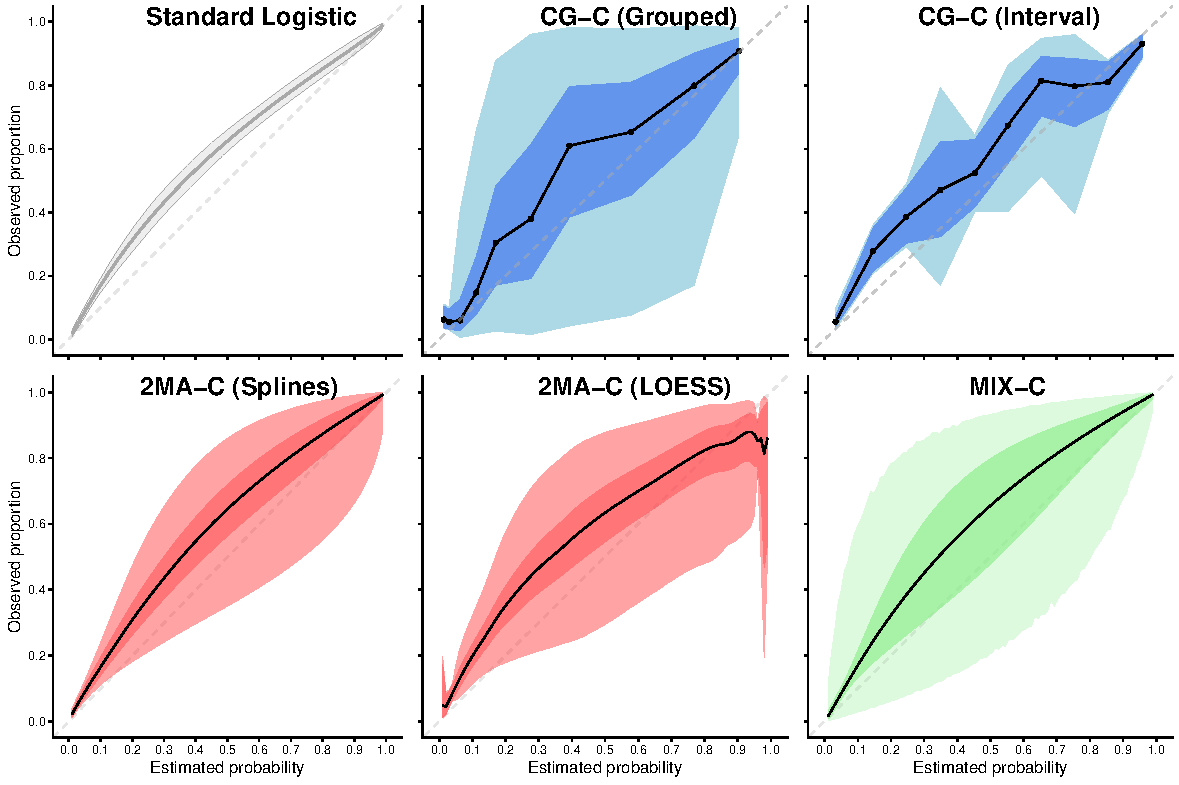
\includegraphics[width=1\textwidth]{figures/ClusteredCalibration/F3.pdf}
\caption[Comparison of traditional plots and introduced methododologies]{Comparison of the standard logistic regression with splines and the three introduced methodologies with CI (bright shaded) and PI (light shaded). Number of quantiles for CG-C were 10, 2MA-C fitted center-specific curves with splines or LOESS, and MIX-C used random intercept and slopes with restricted cubic splines and three knots. The dashed diagonal line indicates perfect calibration.}
\label{fig:4:3}
\end{figure}

\section{Simulation study}
The motivating example showcases the applicability of the methods. However, with real data it is not possible to know the true underlying observed proportion. Therefore, we designed a simulation study to explore the performance of the introduced approaches and compare it with cluster ignorant methodologies.

\subsection{Methods}
The data generating models were based on logistic regression with a random intercept per cluster, hence the formula to obtain the true probabilities was of the form \(\text{logit}\left( \pi\left( x_{ij} \right) \right)\mathbf{=}\beta_{0} + x_{ij}\beta_{1}\mathbf{+}u_{j}\). \(\beta_{0}\) represents the intercept, \(\beta_{1}\) the corresponding effect of covariate \(x\) and \(u_{j}\) is the cluster-specific deviation. We first obtain the true models according to a full factorial design where two factors were varied: little vs strong clustering (\gls{ICC} 5\% or 20\%) and lower vs higher true area under the receiver operating characteristic curve (\gls{AUC};0.75 and 0.9). Event rate was fixed at 30\% for the whole population but varied between clusters according to the variance of the random intercept \(u_{j}\). For each data generating mechanism, we generated data for 200 clusters and 2.000.000 patients (10.000 observations per cluster) and a single normally distributed linear predictor (\(x\)\emph{,} which can be seen as a combination of several predictors) with mean 0 and variance 1. Random effects (\(u_{j})\ \)were also normally distributed with variance according to the desired \gls{ICC}. \gls{ICC} is calculated as the variance of a null random intercept model divided by the total variance, calculated as the addition of the variances of the null random intercept model and the standard logistic distribution \cite{hosmerAppliedLogisticRegression2013a}. \gls{AUC} was controlled by varying the coefficient (\(\beta_{1}\)) and the desired event rate was controlled by modifying the intercept \(\beta_{0}\). We obtained 4 superpopulations by trial and error (Table S1). The code to obtain the superpopulations is available in the \gls{OSF} repository.

In each of the superpopulations we draw 4 scenarios, inspired by real validation or development studies, varying events per cluster (\gls{EPC}) (20 vs 200) and number of clusters (5 vs 30). These scenarios refer to the dataset on which hypothetical prediction models are developed or validated. This results in 16 scenarios overall, by combining all values for \gls{ICC}, \gls{AUC}, \gls{EPC} and number of clusters. We then applied the methods for varying development or varying validation sample size.

\subsubsection{Varying development size}
The clusters and patients within each cluster were selected randomly and the number of patients was selected according to the prevalence and the desired \gls{EPC} (\(n_{j}\) = \gls{EPC} * 1.15 divided by cluster prevalence, we multiply \gls{EPC} to ensure that the desired \gls{EPC} is obtained across all clusters). We developed logistic regression models with restricted cubic splines and 3 knots in these training datasets. Then, we externally validated the calibration of the model in patients from clusters not used for model development in an ideal situation with high number of clusters and high \gls{EPC}. Therefore, we validated models on a random selection of 100000 observations from a random selection of 30 clusters that were not sampled for model development. On average, each cluster contained 1000 events and 3333 observations, but the number of events varied depending on the cluster specific event rate.

\subsubsection{Varying validation size}
Additionally, we validate the models with varying validation sample size. In this case we fixed the model to be validated to a logistic regression model with restricted cubic splines and 3 knots trained with a sufficiently large sample size according to Riley's criteria (N = 1711) from a cluster with average event rate in each of the superpopulations \cite{rileyMinimumSampleSize2021}. Then we validated those models varying \gls{EPC} (20 vs 200) and number of clusters (5 vs 30) in the validation sample.

We applied the \gls{CGC} (grouped and interval), \gls{TMAC} (splines and loess) and \gls{MIXC} approaches to the validation sample in both approaches. For comparison, we also obtained a standard flexible logistic calibration model (i.e. ignoring clustering, see section 2.3) using restricted cubic splines and 3 knots. True risks are obtained using the formula in Table S1, and the true risks in the cluster with the average effect are obtained by setting the random intercept to 0. These true risks can be used to generate true calibration curves per cluster and for the cluster with the average effect. To numerically compare the deviation of the estimated calibration curve from the true one, we calculate the mean squared calibration error (\gls{MSCE}) as the mean squared difference between the estimated observed proportions and the true observed proportions (based on the true risks) in the cluster with the average effect (setting \(u_{j} = 0\)) over a fixed grid of 100 estimated risks (100 evenly spaced points from 0.01 to 0.99) \cite{vanhoordeSplinebasedToolAssess2015}. For \gls{CGC}, the grid contains 10 points by definition. The process was repeated 100 times per scenario.

\subsubsection{Heterogeneity}
We evaluated the coverage of the 95\% prediction intervals. For each of the three methods, using the same grid of values that we used for the \gls{MSCE}, we evaluated whether the true cluster-specific risk (including random effects) falls within the prediction interval at each of the grid points. This means that we obtained the true cluster specific probabilities using the formula in Table S1 and compared for each clustered calibration approach if the prediction interval contained the true values. Coverage was calculated as the proportion over the 200 clusters in the superpopulations.

\subsection{Results}
The median \gls{MSCE} results for varying validation sample size are displayed in Table~\ref{tab:4:2} (multiplied by 100) and Figure~\ref{fig:4:4}. Note that \gls{CGC} focuses on 10 points whereas the other approaches focus on a grid of 100 points, such that \gls{CGC} and the other approaches are not directly comparable. \gls{MIXC} was the best performing approach in all cases. \gls{TMAC} (splines) also performed well in scenarios with high validation sample size. In general, the \gls{MSCE} was better with high \gls{EPC}, low \gls{ICC} and with more clusters in the validation. Standard flexible logistic calibration performed considerably worse in all scenarios, in particular when \gls{ICC} was high. When evaluated on a big validation sample with varying development size the results showed also that \gls{TMAC} (splines) and \gls{MIXC} were the best methods across all scenarios (Table~\ref{tab:4:3} and Figure S9).

\begin{table}
\centering
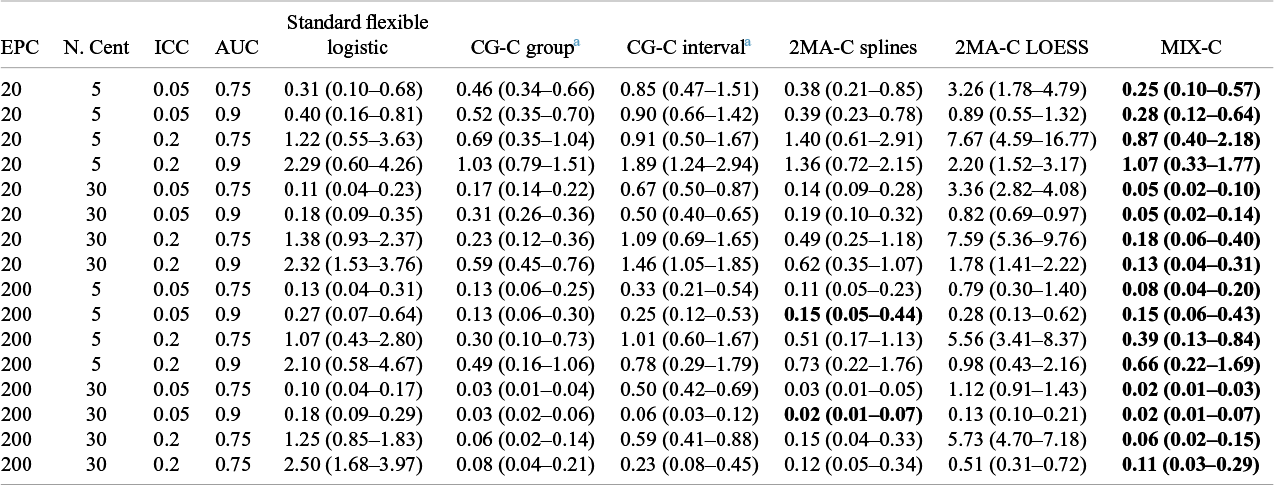
\includegraphics[width=1\textwidth]{figures/ClusteredCalibration/T2.png}
\caption[Median MSCE for varying validation sample size]{Median (IQR) squared difference between true average probabilities and estimated observed proportion (MSCE) with logistic calibration, CG-C (10 groups), 2MA-C, and MIX-C methods for a logistic model varying validation events per center and number of centers. Bold numbers indicate best performance across approaches. MSCE is multiplied by 100.}
\label{tab:4:2}
\end{table}

\begin{figure}
\centering
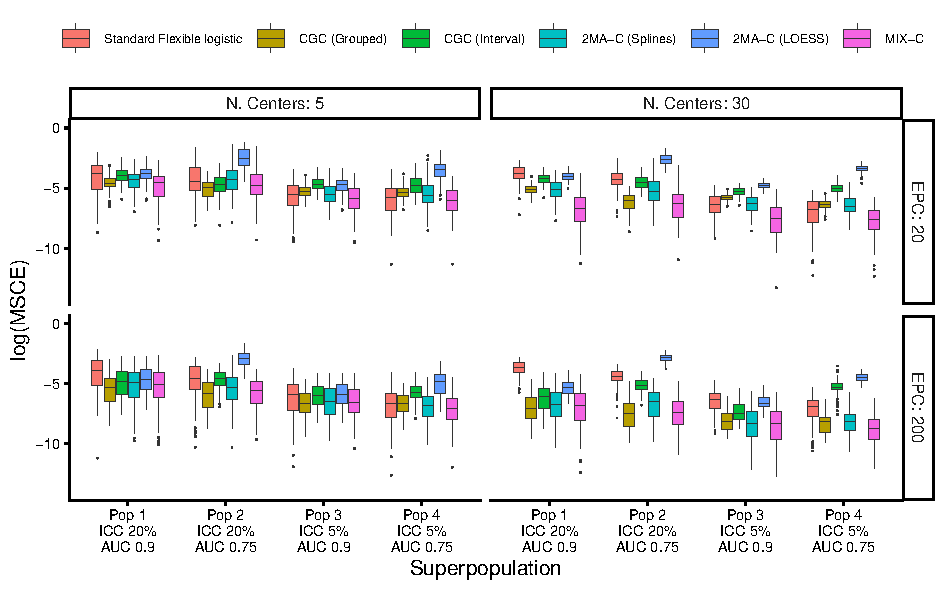
\includegraphics[width=1\textwidth]{figures/ClusteredCalibration/F4.pdf}
\caption[Boxplots of mean squared calibration error]{Boxplots of mean squared calibration error (log) for fixed prediction models varying validation events per center (EPC) and the number of centers in the validation.}
\label{fig:4:4}
\end{figure}

\begin{table}
\centering
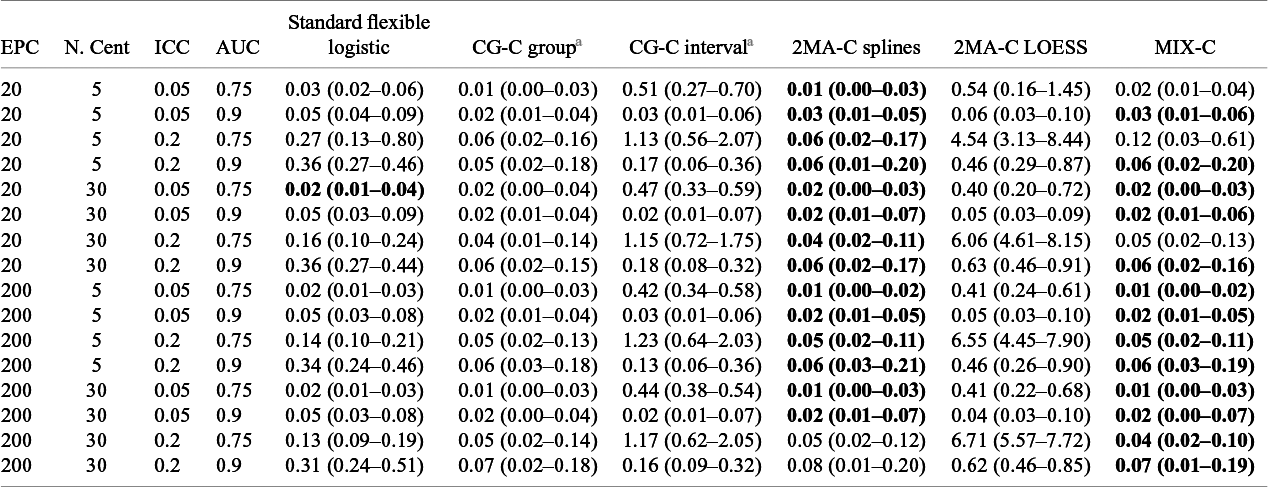
\includegraphics[width=1\textwidth]{figures/ClusteredCalibration/T3.png}
\caption[Median MSCE for varying training sample size]{Median (IQR) squared difference between true average probabilities and estimated observed proportion (MSCE) with logistic calibration, CG-C (10 groups), 2MA-C, and MIX-C methods for a logistic model varying training sample events per center and number of centers. Bold numbers indicate best performance across approaches. MSCE is multiplied by 100.}
\label{tab:4:3}
\end{table}

The prediction interval coverage with varying validation sample was close to nominal with high \gls{EPC} and low \gls{ICC} and when using the \gls{TMAC} (splines) approach (Figure~\ref{fig:4:5}). When \gls{EPC} was high the coverage was close to nominal in the region where validation data was available but very poor at the tails (i.e. regions with few validation data) except for the \gls{MIXC} approach. \gls{MIXC} had correct coverage when \gls{ICC} was high and \gls{AUC} low, too wide prediction intervals when \gls{ICC} was low and too narrow \gls{PI} when \gls{ICC} and \gls{AUC} were high. When \gls{EPC} was low, increasing the number of clusters reduced notably the coverage, especially for the grouped approaches and at the tails. The coverage in the large validation dataset was poor at tails except for \gls{MIXC} (Figure S10). High \gls{AUC} and low \gls{ICC} in development tend to have better \gls{PI} coverage.

\begin{figure}
\centering
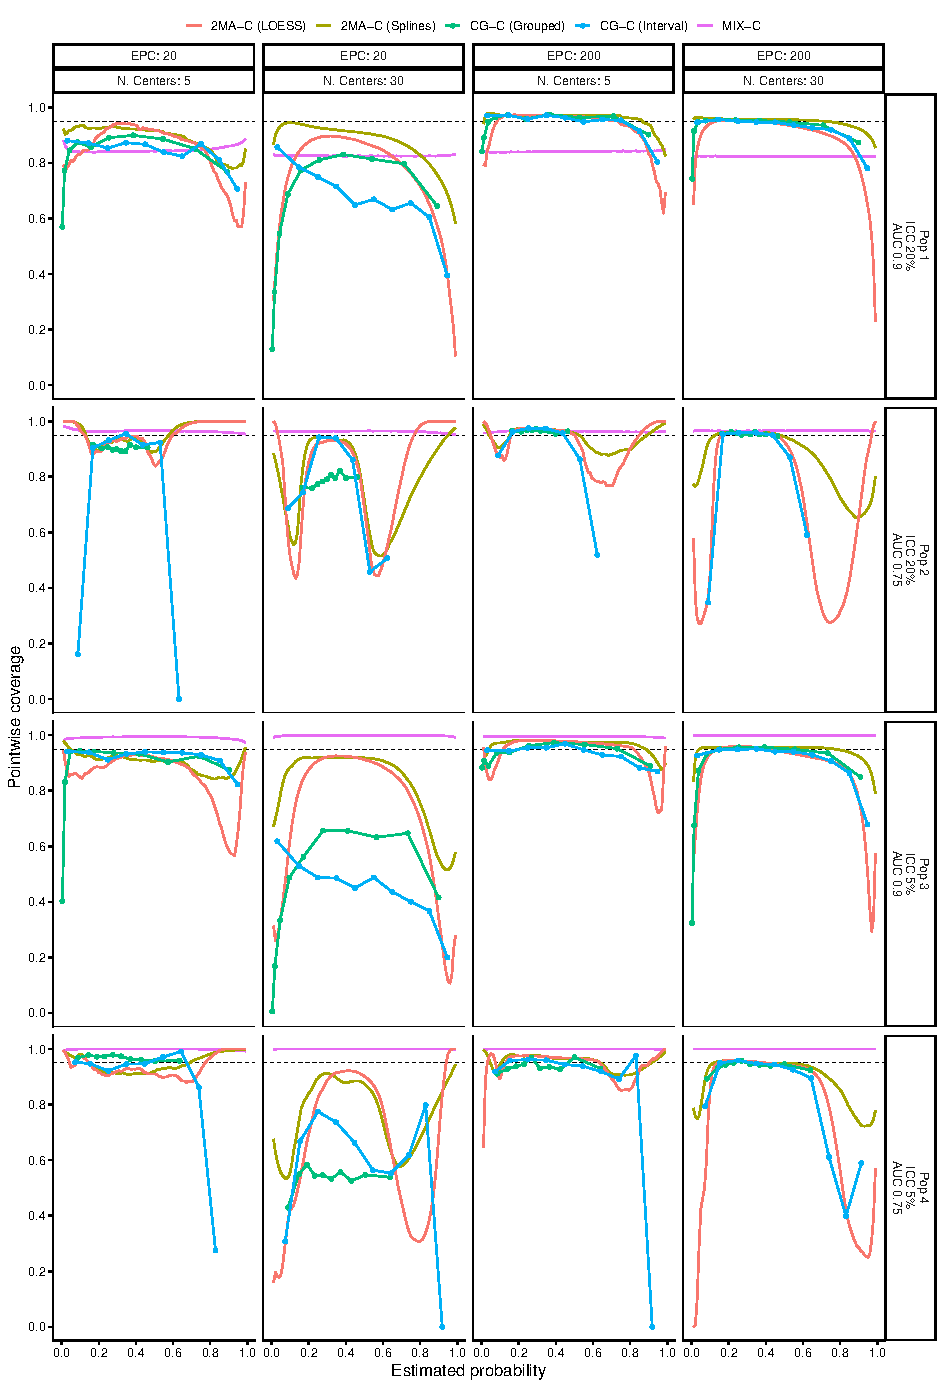
\includegraphics[width=1\textwidth]{figures/ClusteredCalibration/F5.pdf}
\caption[Pointwise prediction interval coverage]{Pointwise prediction interval coverage varying the validation sample size. The model validated is the same in each superpopulation, and it was trained from a center with average event rate and with adequate sample size. The black dotted line indicates nominal coverage (95\%).}
\label{fig:4:5}
\end{figure}

Code and data to reproduce the simulation study and analysis are available in the \gls{OSF} repository \cite{barrenadaOSFClusteredFlexible2024}.

\section{Synthetic data}
The simulation study showed that the methods correctly estimate observed proportions under different logistic \glspl{DGM}. In the real world, the link between outcome and predictors is often not perfectly defined by a linear or logistic function. Therefore, we aim to test the methods in a more flexible situation using a synthetically generated dataset based on the data used in the motivating example.

\subsection{Methods}
To generate synthetic data, we use data from the International Ovarian Tumor Analysis (\gls{IOTA}) consortium that was used to develop prediction models to estimate the risk of malignancy in patients with an ovarian tumor \cite{vancalsterValidationModelsDiagnose2020,vancalsterEvaluatingRiskOvarian2014}. We used the synthpop package in R, which learns the structure of the data and generates a new dataset where individual patient data is masked but the underlying structure is preserved \cite{nowokSynthpopBespokeCreation2016}. We generated synthetic data for 1 million individuals for each of the 10 hospitals separately, and used these synthetic patients as cluster-specific populations (retaining the clustered structure of the original dataset). We generated two true models per center: one based on a logistic regression model with splines for continuous variables, and one based on a random forest model with number of randomly selected parameters per split (mtry) set to three and the depth of the individual trees set to ten (minimum node size) \cite{wrightRangerFastImplementation2017}. Both models were trained on the real data from that center, using the nine \gls{ADNEX} predictors listed above except type of center. The true models were applied to the 1 million synthetic patients, and the outcome was generated with Bernoulli trials based on the true risks of malignancy from the applied models. This means that the same synthetic patient has two true risks and can have two different outcomes. The code to generate the synthetic data is available in the \gls{OSF} repository, but the original data or the synthetic data are not publicly available. The comparison of the real and synthetic data for quality check in one center is presented in Figure S11.

We used the synthetic data to validate the calibration of the published \gls{ADNEX} model without CA125 in each center \cite{vancalsterEvaluatingRiskOvarian2014}. We define 15 scenarios based on the number of centers (2,5,10) and validation data \gls{EPC} (20,100,200,500,1000). We repeat this 1000 times, by randomly drawing validation datasets. If the number of centers was 2 or 5, the centers were randomly chosen as well. In each repetition, we calculate \gls{MSCE} for the two true risks. True center-specific curves are obtained by training flexible calibration models (splines with 5 knots) on all 1 million synthetic patients from that center (Figure~\ref{fig:4:6}). We then compared the center specific estimated observed proportions and the true probabilities per center in a fixed grid of 100 values. The only method that obtains center specific curves borrowing information from other clusters is the \gls{MIXC} method and we compare this to standard flexible calibration with LOESS and restricted cubic splines with 3 knots (Stage 1 of \gls{TMAC}).

\begin{figure}
\centering
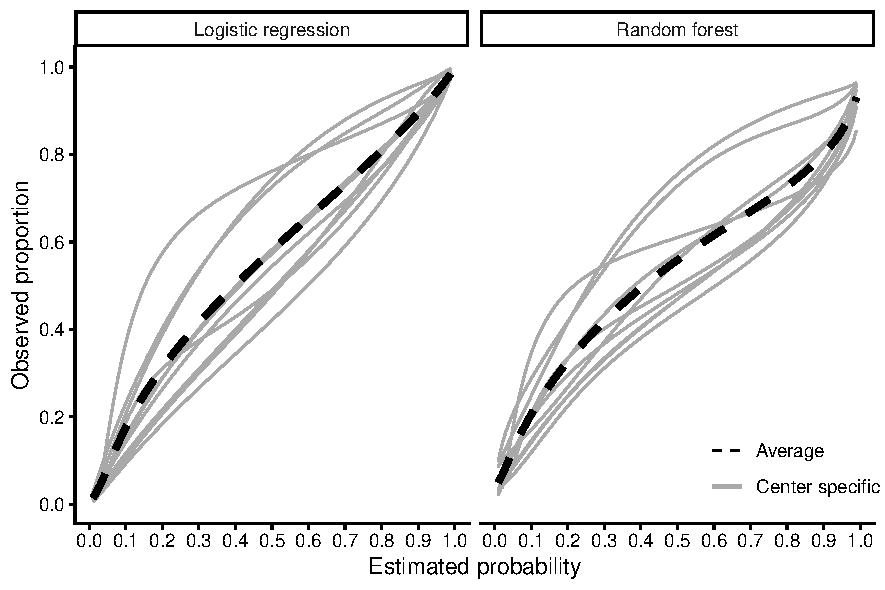
\includegraphics[width=0.8\textwidth]{figures/ClusteredCalibration/F6.pdf}
\caption[Center-specific calibration plots for the synthetic data]{Center-specific (grey) and average true calibration plots for the synthetic data with 1000000 observations per center.}
\label{fig:4:6}
\end{figure}

\subsection{Results}
Median \gls{MSCE} for the synthetic data analysis with 1000 iterations is shown in Table~\ref{tab:4:4} and by center in Figure~\ref{fig:4:7}. \gls{MIXC} was the best performing method in all scenarios when the truth was based on a logistic regression, with splines working equally well in 5 scenarios. When the truth was based on a random forest model \gls{MIXC} was the best with small validation samples (\gls{EPC} < 500) and loess when sample size was above 500 events per center. Borrowing information from other clusters is an example of a bias-variance trade-off and leads to improved accuracy for the estimated cluster-specific curves for clusters with modest sample sizes. Additionally, the performance by approach varied considerably between centers (Figure~\ref{fig:4:7}). That is, the best approach varied by center.

\begin{table}
\centering
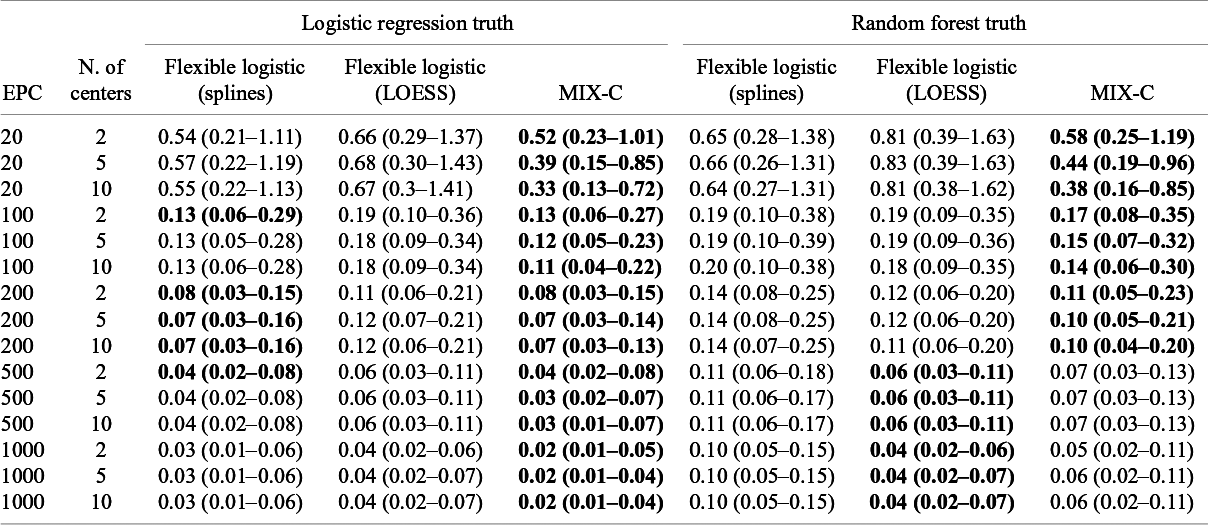
\includegraphics[width=1\textwidth]{figures/ClusteredCalibration/T4.png}
\caption[Median MSCE for center-specific results in the synthetic data]{Median MSCE for the synthetic data study for center-specific results. MSCE is presented multiplied by 100. Bold numbers indicate best performance across approaches.}
\label{tab:4:4}
\end{table}

\begin{figure}
\centering
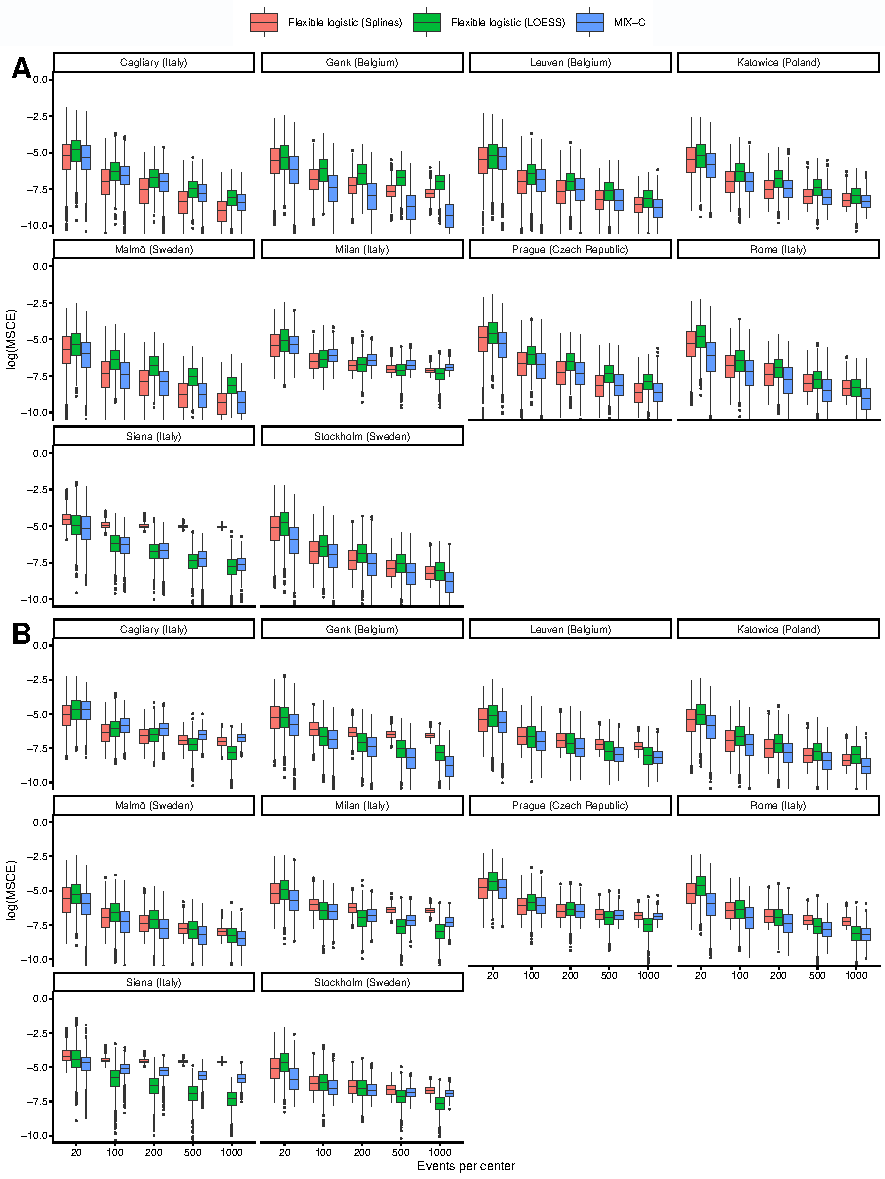
\includegraphics[width=1\textwidth]{figures/ClusteredCalibration/F7.pdf}
\caption[Center-specific log(MSCE) in the synthetic data]{Center-specific results of log(MSCE) by the number of events per center for the logistic truth (a) and the random forest (b) truth.}
\label{fig:4:7}
\end{figure}

\section{Discussion}
Calibration of clinical prediction models is crucial since it is related to the usefulness of the recommended clinical decisions provided by the model \cite{vancalsterCalibrationRiskPrediction2015}. Evaluation of calibration performance is best done with flexible calibration plots \cite{vancalsterCalibrationHierarchyRisk2016,austinGraphicalAssessmentInternal2014}. In this work, we introduced three methods for obtaining flexible calibration plots that account for clustering in the dataset. The first method extended the grouped calibration plot using bivariate random effects meta-analysis (\gls{CGC} method), the second method was a two-step approach in which flexible cluster-specific plots were combined through random effects meta-analysis. We generated cluster-specific plots in two ways: using restricted cubic splines (\gls{TMAC} splines) or LOESS (\gls{TMAC} loess). The third method used a mixed effects logistic calibration model using restricted cubic splines and random intercepts and slopes per cluster (\gls{MIXC}). Through a simulation study and a study using synthetic data from patients with an ovarian tumor, we observed that \gls{MIXC} and \gls{TMAC} (splines) work best to obtain the calibration plot in the cluster with the average effect (simulation study) and \gls{MIXC} for the cluster specific calibration plots (synthetic data). The coverage probability of the prediction interval was suboptimal for all methods and all scenarios with \gls{TMAC} (splines) standing out as the best across scenarios. A disadvantage of \gls{TMAC} (splines) is that the estimated calibration curves per cluster deviated more from the true curves per cluster than those obtained by \gls{MIXC}, which uses shrinkage to obtain better cluster-specific calibration curves. While \gls{CGC} may work well too to obtain a calibration plot in the cluster with the average effect when using 10 groups based on deciles, it worked poorly when using 10 groups based on equal intervals of the estimated risk. However, the grouped approach tends to depend on the number and types of groups, which is undesirable \cite{vancalsterPerformanceEvaluationPredictive2024,arrieta-ibarraMetricsCalibrationProbabilistic2022}. Obviously, the other methods depend on the level of smoothing of the spline or LOESS, but we automatically selected these parameters based on statistical goodness of fit to reduce the modeler's choices. We recommend using \gls{TMAC} (splines) to estimate the curve with the average effect and the 95\% \gls{PI} and \gls{MIXC} for the cluster specific curves, especially when sample size per cluster is limited. In our simulation, \gls{TMAC} (loess) had the worst performance possibly due to the logistic data generation mechanism. In real world the association of outcome and predictors tends to be more complex therefore a more flexible approach could be useful, as shown in the synthetic data with a nonlinear data generating mechanism and large validation sample sizes per cluster. In this work we used the method only for external validation, but the methods also apply to model development with clustered data to explore between-cluster calibration heterogeneity during internal-external validation. We provide ready-to-use R functions to plot the curves and obtain numerical results in the \gls{OSF} Repository , and they will soon be incorporated into the ``CalibrationCurves'' package in CRAN \cite{DeCock2023}.

Munoz and colleagues developed similar methodologies to derive calibration plots in large clustered datasets (preprint published after our initial submission) \cite{munoz2025}. In their work they present four approaches to obtain overall calibration plots. Although their rationale is similar to ours in some cases, the implementation is different. The stacking approach is similar to what we define as flexible curve ignoring clustering (section 2.3), where all the data from different clusters is combined into a single dataset and a calibration model is fitted. Their ``One-step meta-analysis'' approach corresponds to our \gls{MIXC} method where a mixed model is fitted. Their ``two step meta-analysis'' method is similar to \gls{TMAC} but they also present a variant where instead of fitted probabilities the model parameters are aggregated. Finally, they introduced an approach where the calibration model is a Generalized Estimating Equation. None of the methodologies include the estimation of prediction intervals. The work is illustrated with an evaluation of a model to diagnose deep vein thrombosis, but no simulation study is included to evaluate the performance of the methodologies or to compare to our results.

The main strength of our methodologies is the inclusion of a heterogeneity measure through the prediction intervals. These intervals indicate, for every estimated risk, the range within which the observed proportion may fall in a new cluster. It is crucial to differentiate the calibration in the cluster with the average effect with the cluster-specific calibration represented in the \glspl{PI}. Whilst a model can be well calibrated in the cluster with the average effect, this does not necessarily imply that the model is perfectly calibrated in every individual cluster. Statements such as ``the model was well calibrated'' based on the cluster with the average effect calibration plot should be avoided, or at least accompanied by a clarification that this only applies to the summary curve. Using the interpretation of a calibration curve with the average effect for a specific cluster might lead to incorrect decision making. For example, the curve with average effect suggests overestimation of risks but in some cluster the model might be underestimating them. Although no method provided prediction intervals with correct coverage in all investigated simulation scenarios (Figure~\ref{fig:4:5} and S10) they show a more realistic picture than the cluster-ignorant confidence intervals. In general, all methods underestimate the heterogeneity between clusters therefore yielding too narrow prediction intervals, especially for estimated risks far from prevalence and when validation sample size is small. Prediction interval of \gls{MIXC} had an odd behaviour where it tended to have too narrow or too wide \glspl{PI} across the calibration curve. For the rest of approaches, increasing the number of clusters in the validation when events per cluster were low caused the \gls{PI} to be too narrow (Figures S12-S16). More research to fix the suboptimal performance of the prediction intervals is needed where Bayesian based \gls{PI} derivation could be a solution \cite{partlettRandomEffectsMetaanalysis2017,debrayFrameworkMetaanalysisPrediction2019,higginsReevaluationRandomeffectsMetaanalysis2009}. Another limitation concerning \gls{CGC} and \gls{TMAC} is that they present calibration plots based on meta-analysis of independent points. These approaches create the plot joining each pointwise estimate of observed proportion instead of creating a model for the whole plot and therefore are dependent on the number of points. Each of these points represents the calibration in the cluster with the average effect conditional on the estimated risks. We assume that all pointwise estimates form the calibration plot in the cluster with the average effect but in the modelling process each point is independent.

This study is a phase 2 methodological study that focused on the presentation of the methodology and assessments in a limited number of settings \cite{heinzePhasesMethodologicalResearch2024}. Further research should therefore evaluate the methods in more extended settings and applications. For example, simulations could focus on more complex truths, such as multiple predictors with random slopes for their effects on the outcome, continuous predictors with nonlinear associations with the outcome under study, and prediction models based on flexible machine learning methods such as random forests, boosting approaches, or neural networks. Instead of performing a larger simulation study, we decided to focus on synthetic data based on real data from 10 hospitals on women with an ovarian tumor with the aim of building diagnostic prediction models to estimate the risk of malignancy. This data was used to evaluate an existing prediction model, \gls{ADNEX}, which was a multinomial logistic regression model using random intercepts and uniform shrinkage of model coefficients \cite{vancalsterEvaluatingRiskOvarian2014}. In this synthetic data analysis we focused on the cluster specific performance of \gls{MIXC} varying the validation sample. \gls{MIXC} showed good results, especially when sample size is limited, while non-clustered approaches generally performed worse.

\section*{Other information}
\subsection*{Contributors}
Contributions were based on the CRediT taxonomy. Conceptualization: LB, LW, BVC. Funding acquisition: LW, BVC. Project administration: LB. Supervision: LW, BVC. Methodology: LB, LW, BVC, BDCC. Resources: LB. Investigation: LB, LW, BVC. Validation: LB, LW, BVC, BDCC. Data curation: BVC. Software: LB. Formal analysis: LB, LW, BVC. Visualization: LB, LW, BVC. Writing -- original draft: LB, LW, BVC. Writing -- review \& editing: LB, LW, BVC, BDCC. All authors have read, share final responsibility for the decision to submit for publication, and agree to be accountable for all aspects of the work.

\subsection*{Availability of data and materials}
Data and code to reproduce results and figures are available in a public, open access repository (link \url{https://osf.io/aj8ew/}). All data relevant to the study are included in the article or uploaded as supplementary information except the motivating example data and the synthetic data due to privacy concerns.

\subsection*{Funding}
This research was supported by the Research Foundation -- Flanders (FWO) under grant G097322N with BVC as supervisors. LW and BVC were supported by Internal Funds KU Leuven (grant C24M/20/064). LB is supported by a long stay abroad grant from Research Foundation -- Flanders (FWO) under grant V457024N.

\subsection*{Conflicts of interest}
The authors declare that there is no conflict of interest.


\chapter[Fundamental problem of risk prediction]{The fundamental problem of risk prediction for individuals: health AI, uncertainty, and personalized medicine}
% Only include if the thesis is written as a collection of papers
%_________________________
\label{sec:chp_FundamentalProblem}

\glsunset{AI}
\glsunset{ADNEX}
\glsunset{AUC}
\glsunset{IOTA}
\glsunset{RU}

\includegraphics*[width=0.3\linewidth]{logos/arxiv-logo.png}\vspace{0.5cm}

published as: 
\begin{quote}
Barreñada L, Steyerberg E, Timmerman D, Thomassen D, Wynants L, Van Calster B. The fundamental problem of risk prediction for individuals: health AI, uncertainty, and personalized medicine. npj Digital Medicine (submitted).
\end{quote}
\begin{quote}
\textbf{Supplementary material and code} available at \url{https://osf.io/2h9g5/}.
\end{quote}
\vspace{-0.5em}
\noindent\scriptsize\textit{Submitted for the first time: 09/05/2025 \quad Published: --- \quad APC: ---€}
\normalsize\vspace{-0.5em}
%_________________________
\section*{Summary}\label{abstract}

Clinical prediction models for a health condition are commonly evaluated regarding performance for a population, although decisions are made for individuals. The classic view relates uncertainty in risk estimates for individuals to sample size (estimation uncertainty). We show empirically that estimation uncertainty can be strongly dominated by model uncertainty (variability in modeling choices) and applicability uncertainty (variability in measurement procedures and between populations), even for models that perform well at the population level. Estimation uncertainty decreased considerably with increasing training sample size, whereas model and applicability uncertainty remained large. Hence, individual risk estimates are far more uncertain than often assumed. AI should inform, not dictate, care supporting personalization through clinician-patient interaction rather than through inherently uncertain model outputs. 

\newpage

\section{Introduction}

Clinical risk prediction models, which are increasingly based on artificial intelligence (AI), estimate the probability of a medical event occurring in a patient, conditional on a set of predictors \cite{steyerberg2019clinical}. Examples include models to estimate the 10-year risk of coronary heart disease \cite{hippisley-coxDevelopmentValidationQRISK32017}, early mortality in cardiac surgical patients \cite{nashefEuroSCOREII2012}, the risk of ovarian cancer \cite{vancalsterEvaluatingRiskOvarian2014}, the 10-year mortality risk of breast cancer patients \cite{candidodosreisUpdatedPREDICTBreast2017}, or the risk of deterioration in hospitalized patients with COVID \cite{guptaDevelopmentValidationISARIC2021}.

The performance of prediction models is usually assessed at the population level. To make informed decisions for an individual patient, however, the focus is on the risk estimates for that individual. The trustworthiness of individual risk estimates is commonly ignored in practice, and rarely evaluated or quantified \cite{altmanWhatWeMean2000}. We aim to present a structured framework of the key sources of uncertainty in risk estimation for individuals, and to expose the magnitude of uncertainty arising from sources that are typically hidden in practice. We illustrate this with a case study on estimating the risk of cancer in patients presenting with an ovarian tumor.

\section{A framework for uncertainty}

Uncertainty and the concept of `individual risk' have been studied for centuries \cite{sternAccuracyPreoperativeRisk2025,altmanWhatWeMean2000,hackingEmergenceProbabilityPhilosophical2006,finettiTheoryProbabilityCritical1979,vennLogicChance1876,vonmisesProbabilityStatisticsTruth1957,laplacePhilosophicalEssayProbabilities1902,lemeshowOutcomePredictionIndividual1995,hendersonIndividualSurvivalTime2005,steyerbergEquallyValidModels2005}. An individuals' risk of an event as estimated by a prediction model refers to the probability of that event in the subgroup of individuals with the same predictor values. Truly individual risks do not exist because of the `reference class problem': an individual can belong to an infinite number of subgroups. By choosing a different set of predictors to condition on, the reference class changes, and so does the risk. Yet, despite the philosophical challenges in defining a true individual risk, risk estimates are routinely used in practice, making it crucial to understand the different types of uncertainty they carry. For predictive modeling, a basic decomposition of uncertainty is into aleatoric and epistemic uncertainty (Table~\ref{tab:5:1} and Figure~\ref{fig:5:1}) \cite{hullermeierAleatoricEpistemicUncertainty2021,sengeReliableClassificationLearning2014}. Aleatoric uncertainty refers to the inherent random nature of the event we want to predict. Two patients who have the same values for the predictors in the best possible model may still have a different outcome. This does not invalidate the prediction. In contrast, epistemic uncertainty refers to lack of knowledge about the best possible model. We break down epistemic uncertainty for predictive modeling into three key categories: estimation, model, and applicability uncertainty (Table~\ref{tab:5:1}).


\begin{table}
\centering
\small
\caption[Overview of epistemic uncertainty]{Overview of the categories of epistemic uncertainty.}
\label{tab:5:1}
\begin{tabularx}{\textwidth}{>{\raggedright\arraybackslash}p{0.25\textwidth} >{\raggedright\arraybackslash}X >{\raggedright\arraybackslash}X}
  \toprule
  \textbf{Description} & \textbf{Examples} & \textbf{Actions} \\
\midrule
	\textbf{ESTIMATION UNCERTAINTY} & Instability of the fitted model due to finite training sample size. If we collect two datasets from the same population with the same sample size and sampling procedures, and train the same model on both datasets, the estimated model parameters will differ. & Increase sample size; quantify instability (e.g. 95\% confidence intervals or effective sample size) \cite{thomassenEffectiveSampleSize2024}. \\
\addlinespace
	\textbf{MODEL UNCERTAINTY} & Uncertainty due to lack of knowledge about the optimal model specification (model class, feature specification, transformations, selection, hyperparameter tuning). & Improve education about good modeling practice; conduct literature searches and exploratory studies; run pilot comparisons of model classes. \\
\addlinespace
	\textbf{APPLICABILITY UNCERTAINTY (DATA)} & Variability in data collection procedures: differing variable definitions, measurement methods, assay kits, inter-rater variability, and missing-data mechanisms \cite{luijkenImpactPredictorMeasurement2019,agnielBiasesElectronicHealth2018}. & Standardize definitions and measurement procedures; empirically compare measurement methods; invest in data cleaning, linkage, and harmonization. \\
\addlinespace
	\textbf{APPLICABILITY UNCERTAINTY (POPULATIONS)} & Variability between populations in case-mix, prevalence, treatment pathways, and associations between predictors and outcome; population drift over time \cite{davisCalibrationDriftRegression2017}. & Conduct multicenter studies; quantify heterogeneity (leave-center-out CV, meta-analysis with prediction intervals); consider local validation and updating \cite{swaminathanReflexiveRecalibrationCausal2025}. \\
\bottomrule
\end{tabularx}
\end{table}


\begin{figure}
\centering
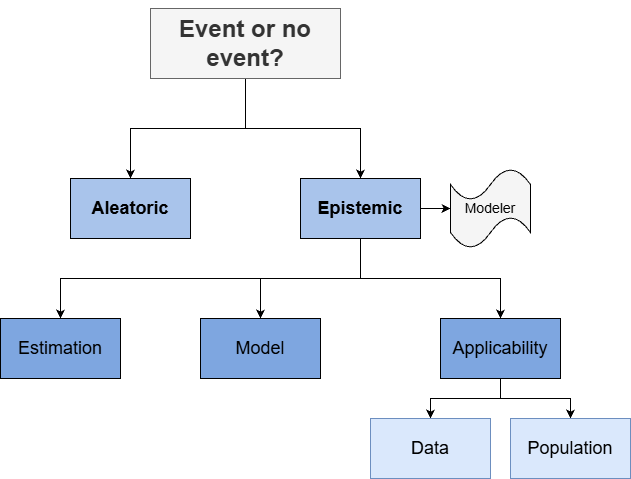
\includegraphics[width=0.9\textwidth]{figures/FundamentalProblem/F1.png}
\caption[A framework of uncertainty when predicting risk for the individuals]{A framework of uncertainty when predicting risk for the individuals.}
\end{figure}



We evaluated population-level performance using the \gls{AUROC} for discrimination, \gls{ECI} for calibration (\gls{ECI}=0 means perfect calibration), and relative utility (\gls{RU}) for clinical utility (\gls{RU}$\leq$0 means no utility) \cite{vanhoordeAssessingCalibrationMultinomial2014,bakerUsingRelativeUtility2009}. To evaluate individual-level variability, we calculated for each patient the 95\% range and \gls{DU} of 59,400 estimated risks per sample size. The 95\% range is the estimated risk at the 97.5th percentile minus the estimated risk at the 2.5th percentile. \gls{DU} is lowest of the proportions of models that yield an estimated risk \textless0.1 vs $\geq$0.1. This is a common threshold in this setting \cite{timmermanESGOISUOGIOTA2021}. If all models yield a risk on the same side of the threshold, there is no \gls{DU} (\gls{DU}=0). If half of the models yield a risk above the threshold, and half below, there is maximal uncertainty (\gls{DU}=0.5). See Appendix 1 in online methods for details.

\section{Results}

\subsection{Estimation uncertainty}

Consider the estimated risk of ovarian cancer for 100 new patients (i.e. patients whose data was not used in model building) according to 100 identical models, each fitted on a different random sample from one population. For some patients, the risk estimates (on a scale from 0 to 1) varied considerably, particularly at small training sample sizes (Figure~\ref{fig:5:2}, left). The mean 95\% range of estimated risks for a new patient decreased from 0.22 for training sets with N=400 to 0.04 for training sets with N=10,000 (Table~\ref{tab:5:2}). When a risk estimate of 0.1 or higher was used as the threshold to recommend surgery for a single new patient, on average 6\% of models trained on a dataset of 400 patients would suggest a different decision than the majority of models. Increasing the training set to 10,000 patients reduced this decision uncertainty to 1\%. We observed that estimation uncertainty is higher and decreases more slowly with increasing training sample size for tree-based models compared to logistic regression (Table~\ref{tab:5:2} and Table S3, Supplementary Figure S3). In contrast to the indicators of uncertainty at the individual level, the population level discrimination and calibration remained rather stable across training sample sizes. The positive population level \gls{RU} indicates the model is useful to support clinical decision-making at all sample sizes.

\begin{table}
\centering
\footnotesize
\caption[Population level performance and individual risk uncertainty]{Population level performance and individual risk uncertainty for the 100 test set patients.}
\label{tab:5:2}
\resizebox{\textwidth}{!}{
\begin{tabular}{l l c c c c c}
\toprule
 &  & \multicolumn{3}{c}{\textbf{Population level performance}} & \multicolumn{2}{c}{\textbf{Individual level uncertainty}} \\
 \midrule

\multirow[c]{2}{*}{\textbf{Source}} & \multirow[c]{2}{*}{\textbf{Training data}} & \textbf{AUROC} & \textbf{ECI} & \textbf{RU} & \textbf{95\% range} & \textbf{DU} \\
&  & \textit{mean (range)} & \textit{mean (range)} & \textit{median$^a$ (range)} & \textit{mean (range)} & \textit{mean (range)} \\
\midrule
\multirow[c]{3}{*}{Estimation} & 400 & .92~(.89;~.93) & .11~(.02;~.21) & .05~(-.61;~.49) & .22~(.01;~.65) & .06~(0;~.49) \\
& 2000 & .92~(.91;~.93) & .11~(.06;~.14) & .20~(-.02;~.49) & .10~(.01;~.36) & .02~(0;~.33) \\
& 10000 & .93~(.92;~.93) & .11~(.10;~.13) & .18~(.02;~.37) & .04~(.00;~.14) & .01~(0;~.31) \\
\addlinespace
\multirow[c]{3}{*}{All sources} & 400 & .92~(.79;~.98) & .11~($<$.01;~.93) & .16~(-2.2;~.82) & .46~(.07;~.91) & .12~(0;~.50) \\
& 2000 & .93~(.84;~.98) & .10~($<$.01;~.68) & .18~(-2.0;~.82) & .41~(.06;~.95) & .11~(0;~.50) \\
& 10000 & .93~(.83;~.98) & .09~($<$.01;~.55) & .18~(-1.5;~.84) & .39~(.06;~.98) & .11~(0;~.50) \\
\bottomrule
\end{tabular}
}
\begin{minipage}{\textwidth}
\vspace{0.5em}
\scriptsize
AUROC: Area under the receiver operating characteristic curve; AUROC 0.5 indicates that the model cannot discriminate between patients with and without ovarian cancer, AUROC 1 indicates perfect discrimination. ECI: Estimated calibration index; ECI is scaled between 0 and 1 with 0 indicating that estimated risks correctly estimate risk at the population level. RU: Relative utility; RU can take on values between $-\infty$ and 1 where positive values indicate the model has clinical utility to support decision making and values $\leq$ 0 indicate that the model has no clinical utility. 95\% range: range of the middle 95\% of risk estimates across all models for one individual; 0 indicates no uncertainty, 1 indicates maximal uncertainty. DU: Decision uncertainty for an individual when using the model at a threshold of 0.1 on the risk of malignancy to suggest a management decision. DU ranges between 0 and 0.5, with 0 indicating that all models suggest the same decision, and 0.5 that half of the models suggest to operate and the other half suggest conservative management.

\textsuperscript{a} We used median because negative values for RU can be very low and distort the results.
\end{minipage}
\end{table}

\begin{figure}
\centering

\includegraphics[width=0.9\textwidth]{figures/FundamentalProblem/F2.png}
\caption[Uncertainty in estimated risks for individual patients]{Visualization of the uncertainty in the estimated risks for individual patients. Panels on the left show estimation uncertainty for the main model based on training sample sizes of 400 (top), 2000 (middle) and 10000 (bottom). Each panel contains the individual estimated risks (y-axis) for 100 test patients (x-axis) by 100 models based on randomly selected training datasets. The main model used unpenalized logistic regression with restricted cubic splines, with regression imputation for missing CA125, no variable selection, using training data from Leuven and with lesion size measured using the maximal diameter. Panels on the right show the total uncertainty for all 59,400 models. Each panel contains the individual estimated risks (y-axis) for 100 patients (x-axis) by 59,400 models based on combinations of modeling strategies, data properties, populations included at training (Supplementary Table S1) and on randomly selected training datasets. This means that each of the 100 patients has 59,400 predicted estimated risks.}
\label{fig:5:2}
\end{figure}

\subsection{Model and applicability uncertainty}

When also acknowledging model and applicability uncertainty, the differences in estimated ovarian cancer risks for any single patient from a total of 59,400 models were considerably larger than when acknowledging estimation uncertainty alone (Figure~\ref{fig:5:2}, right). Even when the training sample size was 10,000, the 95\% range in risk estimates for a single patient was on average 0.39 (range 0.05 to 0.99). The highest 95\% risk range for a single patient was 0.99, nearly covering all possible risk estimates between 0 and 1.

In contrast to approximation uncertainty, increasing the training sample size led to minimal reductions in model uncertainty and applicability uncertainty. On average, 12\% of models trained on 400 patients would lead to a different clinical decision for a single patient than most models suggest. When training was done on data of 10,000 patients, the decision uncertainty was still 11\%. Note that this is substantial compared to the maximum decision uncertainty of 50\% (when 50\% of models suggest to operate and 50\% of models suggest not to operate). Findings were similar for any class of models (Supplementary Table S3).

The mean \gls{AUROC} (0.92-0.93) and \gls{ECI} (0.09-0.11) values were similar to the values observed when we only considered estimation uncertainty (Table~\ref{tab:5:2}). Detailed results about estimation, model and applicability uncertainty available in Online Methods (Synthetic data: Supplementary Figures S3-S6; real data: Supplementary Figures S7-S10 and Supplementary Tables S4-S5).

\section{Discussion}

Precision medicine aims to target interventions towards the specific characteristics of the individual. In this context, prediction models and \gls{AI} algorithms can be valuable to improve decision making. Our study shows that, even though prediction models may perform very well at the population level (high discrimination, good calibration and clinical utility to support decisions), the uncertainty in estimated risks and suggested decisions for a single patient is often uncomfortably large.

Calibration assesses whether estimated risks correspond to observed proportions for (sub)groups of patients, typically using calibration metrics and plots, but does not inform on the uncertainty of risk estimates for an individual patient. The classic approach towards uncertainty assessment for an individual involves confidence intervals or other quantifications of variability that assume that modeling, data, and population decisions are fixed (estimation uncertainty, Table~\ref{tab:5:1}) \cite{rileyStabilityClinicalPrediction2023,thomassenEffectiveSampleSize2024,kompaSecondOpinionNeeded2021}. Recent research on clinical prediction models has focused on estimation uncertainty, i.e. instability as a function of sample size \cite{rileyStabilityClinicalPrediction2023,rileyClinicalPredictionModels2023,rileyUncertaintyRiskEstimates2025}. We demonstrated that the magnitude of model uncertainty and applicability uncertainty may extend far beyond estimation uncertainty. Estimation uncertainty differs from other sources of epistemic uncertainty in two aspects. First, it reduces more strongly with increasing sample size than other sources of uncertainty. Second, it can be visualized and quantified, whereas other sources are mostly invisible and hardly quantifiable. A few studies highlighted that modeling choices including model class, predictors, and missing data imputation techniques may impact on individual risk estimates \cite{ledgerMulticlassRiskModels2023,pateUncertaintyUsingRisk2019,liConsistencyVarietyMachine2020}. In the current analyses, we quantified how data-related choices (in measurement, definition and populations) further impact uncertainty. The number of decisions that are taken to develop a model is potentially infinite, yet we usually only see one specific model.

It may seem paradoxical that using prediction models for decision making can benefit outcomes at a population level without having trustworthy risk estimates for individuals from that population. This may cause skepticism about the acceptability of data-driven clinical decision support tools, either based on classical regression approaches or novel \gls{AI} algorithms. We argue that such skepticism is not needed. Clinical utility at the population level, for example in terms of cost-effectiveness, is sufficient to warrant the use of a decision strategy based on a model. We may need to accept that two models may have the same clinical utility yet very different risk estimates for the same individual, often to the extent that model A recommends treatment initiation, but model B does not. The enormous uncertainty on the individual level does have consequences. First, the uncertainty should be acknowledged and considered when discussing risks and treatment options with patients. Given the considerable impact of poorly quantifiable model and applicability uncertainty, further research is needed on how to integrate model predictions in the shared decision making process. Second, while we should strive to reduce epistemic uncertainty in clinical prediction models, we must also recognize and accept it as an unavoidable element of medical decision-making. Finally, we should be humble regarding the promises of personalized medicine \cite{sennStatisticalPitfallsPersonalized2018}. Health \gls{AI} will always provide highly uncertain group level estimations based on their training data, even if the group is defined very narrowly. As a consequence, the estimated risk for the individual is not personalized, yet the shared decision making based on this estimation can be.

Researchers have a variety of tools at their disposal to reduce or embrace epistemic uncertainty, listed in Table~\ref{tab:5:1}. First, to reduce estimation uncertainty, we need to develop models on sufficiently large sample sizes \cite{tsegayeLargerSampleSizes2025}. Whereas there are elegant sample size calculation procedures for prediction models based on regression, such procedures are lacking for machine learning algorithms, which may generally require large sample size to allow for flexible modeling \cite{rileyCalculatingSampleSize2020,vanderploegModernModellingTechniques2014}. Further, methods that allow prediction abstention due to uncertainty have been proposed \cite{kompaSecondOpinionNeeded2021,myersIdentifyingUnreliablePredictions2020}. Even though not all sources of uncertainty are included, it may be a good start to abstain from predictions based merely on estimation uncertainty, for example requiring at least an effective sample size of 10 patients per prediction \cite{rileyUncertaintyRiskEstimates2025,thomassenEffectiveSampleSize2024}. Second, a better agreement and education about good prediction modeling practices could reduce model uncertainty, including the effects of modeler uncertainty, to some degree. Third, to reduce data uncertainty, the use of prospective study designs can help. Retrospective studies tend to have increased uncertainty regarding the definition, measurement procedure, and availability of relevant predictors and outcome variables. Prospective studies, including randomized controlled trials, typically allow for better standardization of definitions and measurement protocols \cite{steyerbergPrognosisResearchStrategy2013}. For example, a set of `terms and definitions' has become standard in the field of ovarian tumors \cite{timmermanTermsDefinitionsMeasurements2000} and `common data elements' have been defined for traumatic brain injury studies \cite{maasOpportunitiesChallengesHighQuality2022,maasStandardizingDataCollection2011}. While sample size is important for model development, data quality should be prioritized over quantity for clinical prediction model development. Although a huge dataset further reduces estimation uncertainty, it may increase data uncertainty due to data quality problems. Fourth, population uncertainty may be exposed by assessing population differences and performance heterogeneity across sites in multicenter development and validation studies \cite{vancalsterThereNoSuch2023}. Monitoring and updating of prediction models can improve local performance and further decrease uncertainty. Ideally, this includes assessing the causes of the heterogeneity and performance changes over time \cite{youssefExternalValidationAI2023,swaminathanReflexiveRecalibrationCausal2025}.

The strength of our demonstration on ovarian cancer diagnostic modeling is the extensive investigation of different types of uncertainty on empirical data, and its presentation in easy-to-interpret metrics and simple visualizations. At the same time, this approach has a few limitations. First, we were constrained by the available data in our choices related to data and population uncertainty, likely leading to an underestimation of applicability uncertainty. Second, to investigate the results for models built on large training datasets, we created a larger synthetic dataset with identical properties as the original dataset. Third, the event of interest in our dataset was relatively common (37\% of tumors were malignant), which yields larger values for the 95\% range compared to situations where the event is rare. Of note, smaller 95\% ranges in cases with rare events may still affect decision uncertainty, if the decision threshold falls around instable predictions. Fourth, diagnostic models for ovarian malignancy have high \gls{AUROC} values (above 0.9). While higher levels of uncertainty might be present for prediction problems with lower discrimination, the amount of individual risk uncertainty is striking for a model that is well able to distinguish between patients with the event and patients without it at the population level. Finally, although we considered a large number (594) of scenarios, more scenarios could have been conceived. For example, we did not vary the set of six predictors, and our variations in the tree-based algorithms were less extensive than those for the logistic regression analysis. These characteristics of the data and selected scenarios enforce the conclusions of our study, given that most of these issues have most likely underestimated the full uncertainty.

In conclusion, a fundamental problem in risk prediction is that individual risk estimates may be highly uncertain, even for models with high discriminatory ability that improve outcomes for the population when used to guide decision making. The uncertainty for predictions at the individual level will often be considerably larger than suggested by classic uncertainty measures such as 95\% confidence intervals or novel measures such as effective sample size \cite{thomassenEffectiveSampleSize2024}. This uncertainty does not invalidate the clinical utility of well-developed prediction models at a population level, but urges great caution when interpreting and discussing risk estimates with individual patients in clinical practice.



\subsection*{Funding} This research is supported by Research Foundation -- Flanders (FWO) grants G097322N, G049312N, G0B4716N, and 12F3114N to BVC and/or DTi, KU Leuven internal grants C24M/20/064 and C24/15/037 to BVC and/or DTi, ZoNMW VIDI grant 09150172310023 to LW. DTi is a senior clinical investigator of FWO. No funding source had any role in the study design, data collection,data analysis, data interpretation, writing, or submission of this report.

\subsection*{Author contributions} Conceptualization: BVC. Methodology: LB, ES, LW, DTh, BVC. Investigation: LB, BVC. Visualization: LB, BVC. Funding acquisition: DTi, LW, BVC. Project administration: LB. Supervision: ES, BVC. Writing -- original draft: LB, LW, BVC. Writing -- review \& editing: LB, ES, DTi, DTh, LW, BVC.

\subsection*{Competing interests} Authors declare that they have no competing interests.

\subsection*{Data and materials availability} Synthetic and real data are not publicly available, but we provide the individual risk estimations of all the different models and explanatory code to reproduce all the results in this work in the OSF repository (https://osf.io/uxvhq/)

\chapter[Cost-based variable selection]{Cost-based variable selection to improve clinical utility of prediction models}
\label{sec:chp_varselection}

\begin{flushleft}
{\huge\sffamily In preparation}
\end{flushleft}

as: 
\begin{quote}
Barreñada L, Vickers A, Steyerberg E, Timmerman D, Wynants L, Van Calster B. Cost-based variable selection to improve clinical utility of prediction models. Diag. Prog. Res. (submitted).
\end{quote}
% \vspace{-0.5em}
% \noindent\scriptsize\textit{Submitted: X/X/X \quad Published: -- \quad APC: XXX€}
% \normalsize\vspace{-0.5em}

\section*{Summary}\label{abstract}
Clinical prediction models guide diagnostic and prognostic decision-making. However, traditional variable selection methods rely primarily on statistical properties, often ignoring clinical utility and measurement costs. This study introduces a novel variable selection algorithm that selects predictors by maximizing harm-adjusted Net Benefit (NB). By incorporating the "test tradeoff", the specific harm or clinical cost associated with measuring a predictor, into the NB calculation , the algorithm evaluates predictor subsets to identify the clinically optimal model. For high-dimensional datasets, a backward elimination extension is provided, alongside a permutation-based NB variable importance metric to guide selection when harms are difficult to quantify. Demonstrated through a real world ovarian cancer dataset, the utility-guided approach favors simpler, cost-effective models, demonstrating that statistical performance does not necessarily equate to optimal clinical cost-utility.

\newpage

\section{Introduction}

Determining a patient's condition based on their current characteristics is called diagnosis and is key to initiate any treatment and minimize future complications. Different conditions require exploring different characteristics. For example, a bone fracture can be diagnosed through medical imaging and COVID-19 through a PCR test. Clinical prediction models are statistical tools that estimate the probability that a patient has or will develop a condition in the future \cite{steyerberg2019clinical}. These models try to link the outcome (event or condition) with a series of predictors in a dataset, a task often called supervised learning \cite{jamesIntroductionStatisticalLearning2021}. These predictors should be information readily available at the time of diagnosis, not too costly to measure and measured with reasonable precision \cite{steyerberg2019clinical}. However, there might be a vast number of predictors that meet these criteria and selecting among them is needed \cite{chowdhuryVariableSelectionStrategies2020}.

Variable selection, best subset selection, feature selection, and feature engineering are terms used in prediction modelling to describe the process of selecting which predictors to use when training a model. Different approaches for variable selection have been presented. Heinze and colleagues \cite{heinzeVariableSelectionReview2018} categorized methods into five groups based on the criteria to select the variables: (1) based on significance testing, (2) based on information criteria (e.g.\ AIC, BIC), (3) based on penalized likelihood (e.g.\ LASSO, elastic-net), (4) based on change-in-estimate or performance (e.g.\ backward elimination, stepwise selection), or (5) based on background or domain knowledge. Across machine learning literature, it is often observed that variable selection methods are grouped into filter, wrapper and embedded methods \cite{Nguyen2025Vol1}. Filter methods use statistical properties to select variables and are therefore equivalent to significance testing and information criteria-based approaches. Wrapper methods, in contrast, use model performance to select the best subset, which corresponds to Heinze's change-in-estimate criterion. Finally, embedded methods perform variable selection as part of the model training; this includes penalized likelihood but also other approaches such as feature importance calculation in tree-based or genetic algorithms \cite{archerEmpiricalCharacterizationRandom2008,zhangVariableSelectionLogistic2018}. This work will focus on change-in-estimate or wrapper methods for variable selection in clinical prediction models.

To be used in clinical practice, prediction models need to show good performance in external validation in terms of discrimination (area under the ROC curve), calibration (calibration plot), and clinical utility (Net Benefit) \cite{calsterPerformanceEvaluationPredictive2024}. Variable selection is usually performed by considering only the statistical properties of the predictors (filter methods), without accounting for the clinical benefit or utility. Utility refers to the quality of decision-making when a risk model is used to decide whether a patient requires treatment \cite{vancalsterReportingInterpretingDecision2018}. Regarding model validation there is increasing awareness that classical statistical measures are insufficient \cite{steyerberg2019clinical,calsterPerformanceEvaluationPredictive2024}. Models that are not clinically useful are more likely to be forgotten quickly or even never be implemented in real practice \cite{wyattCommentaryPrognosticModels1995}. Consequently, we aim to include clinical utility in the model development process through a clinical utility guided variable selection.

Preliminary efforts to add utility to variable selection have struggled with the generation of utility values and the complexity of the methods  \cite{fouskakisBayesianVariableSelection2009}. Fouskakis and colleagues proposed using stochastic optimization to select the model with the best cost-adjusted Bayesian Information Criterion (BIC). The cost-adjusted BIC extends standard model selection by penalizing the total measurement cost of predictors rather than solely the number of variables included. However, implementing this method requires the specification of a cost-penalized prior, a task that proves difficult for clinicians who must quantify the trade-off between statistical gain and data collection burden.

Utility values, relating to misclassification costs (i.e., the benefit of treating the diseased and the harm of treating the healthy), are hard to elicit at an absolute scale. However, it is known that the ratio of harm to benefit is directly related to the risk threshold for classifying a patient as high risk \cite{vancalsterReportingInterpretingDecision2018}. Net Benefit (NB), a simple metric for clinical utility, uses this relationship. NB is calculated as benefit minus harm multiplied by the exchange rate, or harm-to-benefit ratio \cite{vickersDecisionCurveAnalysis2006}. In statistical terms, this is the number of true positives minus the number of false positives weighted by the exchange rate. This exchange rate reflects how many false positives a clinician is willing to accept per true positive. For example, if a surgeon is willing to perform 9 surgeries on benign tumors to catch 1 malignant tumor, the exchange rate is 1/9, corresponding to a 10\% risk threshold. However, NB should often be presented across a range of thresholds, given variability across clinicians and settings \cite{vickersSimpleStepbystepGuide2019}. NB is a semi-proper metric. A proper metric is one where the expected value is maximized when the model used is correct. NB is semi-proper because it can also be maximized by some incorrect models, provided the imperfect model perfectly classifies at the decision threshold \cite{calsterPerformanceEvaluationPredictive2024}. The use of NB and related metrics to evaluate a new variable was discussed by Baker and colleagues several years ago \cite{bakerEvaluatingNewMarker2012}. However, it has never been implemented as a variable selection algorithm for clinical prediction models.

The aim of this paper is therefore to develop a simple and interpretable variable selection algorithm based on clinical utility to determine the predictors to include in the model. Additionally, we will explore the effect on performance of this method with respect to traditional procedures. We will use and implement the method in the context of a logistic regression to estimate the probability of a binary outcome, but the rationale extends to more flexible machine learning or AI probabilistic algorithms.

\section{Methodology}

\subsection{Algorithm}

The problem we aim to address is defined as follows: given a set of predictors and a modelling algorithm we seek the subset of predictors that maximizes the net benefit:

\begin{equation}
\underset{\mathbf{S} \subseteq \mathbf{P}}{\operatorname{argmax}} \widehat{NB}(\mathbf{S}, \mathbf{M}, t)
\end{equation}

Here, $\widehat{NB}(\mathbf{S}, \mathbf{M}, t)$ denotes the (adjusted) net benefit of algorithm $\mathbf{M}$ with $\mathbf{S}$ predictors for the benefit-harm trade-off $t$. The $t$ parameter may be a single value, or a range of clinically relevant values specified based on clinical context. In cases where a range of values is used, we want to maximize the average NB across that range. This is the general rationale for the methodology; however, we will focus here on the specific case where a logistic regression model is used as the modelling algorithm.

The proposed variable selection algorithm does not involve modifying coefficient estimation, since the logloss minimisation (or log-likelihood maximisation) is known to provide coefficients with good properties. Therefore, the proposed algorithm works as follows:

\begin{enumerate}
\item Define all possible model combinations based on the predictors
\item Assign a test tradeoff or harm to each predictor or group of predictors to adjust the NB accordingly. If the harm is unknown, this can be 0 and unadjusted NB will be used
\item Train models and evaluate their net benefit using cross validation with folds (default is 5)
\item This step can be parallelized to reduce computation time
\item Nonlinearities can be addressed with restricted cubic splines
\item Interactions can be included; we limit this option to either all pairwise interactions or no interactions. If interactions are included:
\item Rank the models based on NB and select the model with optimal NB
\end{enumerate}

Code implementing the Net Benefit based variable selection and the associated visualizations is available in the open-source R package NBvarsel (\url{https://lasaibarrenada.github.io/NB_varsel/}, Box~1).

\begin{codebox}[Box 1: Implementing the Methodology in R]
n <- 500
df <- data.frame(
	X1 = rnorm(n),
	X2 = rbinom(n, 1, 0.7),
	X3 = rnorm(n),
	X4 = rbinom(n, 1, 0.5)
)
df$y <- rbinom(n, 1, plogis(2 + 1*df$X1 + 1.5*df$X2 + 0.2*df$X3))

## Step 1: Install the package (once)
# install.packages("NB_varsel")
library(NB_varsel)

## Step 2: (Optional) Define harms for predictors
harms <- c(X1 = 0.1, X2 = 0.05, X3 = 0.0001, X4 = 0)

## Step 3: Run the core variable-selection routine
result <- nb_varsel(
	data = df,
	outcome_var = "y",
	costs = harms,
	mode = "exhaustive",
	folds = 5,
	permutations = TRUE,
	allow_parallel = FALSE
)

## Step 4: Visualisations (built-in)
all_subset_plot(result$all_models)
VIF_plot(result$all_models, color = "darkgreen")
\end{codebox}

\subsection{Large dimensional settings}

The algorithm presented in Section~2.1 becomes computationally too demanding when the number of candidate predictors increases. For a dataset with 20 candidate predictors, there are more than one million predictor combinations; consequently, the method fits 5 million models when using 5-fold cross-validation. In most trials or observational studies, the sample size is limited; therefore, the number of candidate predictors should also be kept small. Our methodology should always be used in compliance with these sample size criteria as explained in Section~2.2. However, in those cases where the dimensionality of the data is large (e.g.\ electronic health records), we propose an extension of the methodology that we called groupwise (as opposed to exhaustive) net benefit variable selection.

In this extension, instead of calculating all the possible combinations, we use backward elimination with a number of predictors per step specified ($k$), yielding a total of $\binom{p}{k}$ model combinations per step. The fastest version ($k = 1$) therefore would fit $p$ models by removing a single predictor in the first iteration. Then the model with best performance is selected, if that model is the model where all predictors are used, that is selected as the best model, else the predictor(s) that were removed in the model with best performance are removed and the process is iteratively repeated until reaching the optimal model. Allowing values of $k$ higher than one is highly recommended if there is intuition of important interaction effects between predictors.

\subsection{Note on Sample size}

Across systematic reviews of prediction model development and validation studies, a common issue is that there is no rationale for the sample size used \cite{barrenadaADNEXRiskPrediction2024,wynantsPredictionModelsDiagnosis2020}. International guidelines for prediction modelling, such as TRIPOD+AI and PROBAST+AI, recommend always justifying sample size \cite{collinsTRIPODAIStatementUpdated2024,moonsPROBASTAIUpdatedQuality2025}.

The ratio of the number of events and potential number of predictors is called events per variable (EPV) or events per potential predictor (EPP). We prefer the latter because it explicitly states that its value should always be based on potential predictors, prior to data-driven variable selection; otherwise, the coefficients will be biased  \cite{steyerbergLogisticRegressionModeling2011}. In traditional logistic and linear regression, EPP indicates relationship between the number of coefficients to be estimated and the amount of available information. The first recommendations indicated that an EPP of greater than ten was adequate \cite{concatoImportanceEventsIndependent1995,peduzziSimulationStudyNumber1996}. Some years later, several authors disputed this rule, concluding that there is no single EPP rule that would guarantee accurate estimation \cite{vittinghoffRelaxingRuleTen2007,courvoisierPerformanceLogisticRegression2011,vansmedenNoRationale12016}.

Moving beyond rules of thumb, Riley and colleagues have developed several minimum sample size calculation techniques for developing and validating multivariable binary, continuous and time-to-event models \cite{archerMinimumSampleSize2021,pateMinimumSampleSize2023,rileyMinimumSampleSize2022,rileyEvaluationClinicalPrediction2024a,rileyMinimumSampleSize2019,rileyMinimumSampleSize2019a}. Recently, the group has published a general framework that applies both to linear models and to more flexible AI-based algorithms such as random forests \cite{rileyGeneralSampleSize2026}, that had shown to be more ``data hungry'' \cite{austinRelativeDataHungriness2024,vanderploegModernModellingTechniques2014}. These criteria are based on overfitting and optimism control and precise estimation of the intercept.

When sample data is limited, a two-stage approach is often recommended: first selecting a subset of predictors based on subject matter knowledge and then performing a data-driven variable selection \cite{harrellRegressionModelingStrategies2015,steyerberg2019clinical}. Because it is prone to overfitting like any data-driven process, the methodology presented here must always adhere to the recommended minimum sample size.

\subsection{Test harms}

The concept of placing benefit and harm on the same scale is the principle of net benefit (NB) and decision curve analysis (DCA), yet it has not been applied directly to variable selection. In this work, we aim to introduce this concept in model development by defining a harm adjusted NB. Harm is therefore accounted for twice. First, to calculate NB, we set a threshold that should be related to the test harm (harm of misclassifying a patient). Second, the harm of measuring a predictor is introduced in the NB scale by quantifying the minimal expected benefit required to measure a variable. The harm of misclassifying a patient is widely discussed in the literature \cite{avickersSimpleStepbystepGuide2019vickersDecisionCurveAnalysis2006}. The harm of measuring a predictor can be quantified as the number of tests that a doctor is willing to perform to find an event. If the number is higher, then the cost of the predictor is lower. However, specifying this number upfront might be difficult, therefore, the difference in NB ($\Delta NB$) can be used to derive the test tradeoff (TT). TT is the minimum number of tests per true positive that we have to accept to make the model worthwhile given its cost\cite{vancalsterReportingInterpretingDecision2018}. TT is defined as:

\begin{equation}
TT = \frac{\Delta NB}{q \cdot (1-q)}
\end{equation}

where $\Delta NB$ is the NB difference between the model with the additional predictor and the model without the predictor. Imagine we have a model that predicts risk of ovarian cancer with age and ultrasound measurements of the lesion that has a NB of 0.2. We wonder whether measuring CA125, that requires a blood sample, and including it in the model is cost-effective from the NB perspective. Given the monetary costs and test burden, practitioners suggests that they would be willing to measure CA125 in 100 patients to find an event. This means that we would be willing to include the predictor only if the NB increases by at least 0.01 ($\Delta NB > 0.01$). By doing so, the researcher can specify the harm in terms of how many tests per true positive are needed to justify the inclusion of that predictor. For some predictors, such as age or sex, the harm is minimal, hence the TT can be high, meaning that almost any improvement justifies their inclusion. However, other predictors might have a higher associated harm such as a CT-scan which involves monetary costs, discomfort, exposure to radiation, etc. Harmful predictors have low TT, therefore the expected increase in utility must be higher. Quantifying these harms might be difficult and will have an important impact on the models. Some predictors might have shared harms; for instance, a single blood sample could extract information on several predictors. In those cases, the harm of only one or all of those predictors is identical, and the adjusted NB is calculated accordingly. If harms are omitted, the model would select variables based solely on standard NB.

\subsection{Variable importance}

When the test tradeoff or $TT$ is difficult to quantify, an alternative approach to help decide which variable to include in a model is computing each variable's contribution to the clinical utility. Variable importance is typically assessed using the statistical properties of the model being analysed. For instance, in a logistic regression model, coefficients can be used to compare the relative contribution of each predictor, while in random forest the Gini importance is often used to rank predictors by their contribution to the reduction of impurity. Other model-agnostic procedures have been proposed in the explainable AI field \cite{dwivediExplainableAIXAI2023}, with the SHAP (SHapley Additive exPlanations) values and Local interpretable model-agnostic explanations (LIME) being arguably the most popular \cite{lundbergUnifiedApproachInterpreting2017,ribeiroWhyShouldTrust2016}.  However, these techniques assess variable importance based on predicted probabilities rather than the clinical utility of the model.

In his seminal paper introducing random forests, Breiman introduced permutation variable importance \cite{breimanRandomForests2001}. The algorithm proceeds as follows:

\begin{enumerate}
\item A model is trained on training data
\item The performance of the model is evaluated on test or unobserved data
\item The performance of the model on test data is recalculated by randomly shuffling (permuting) values of a predictor $P$
\item The variable importance of $P$ is the difference between the performance on the true dataset and on the permuted dataset
\end{enumerate}

We apply this approach to calculate the average contribution of each predictor to the Net Benefit across the different predictor combinations evaluated. The permuted performance is calculated within the same $k$ folds of the cross-validation to ensure that the permuted and original performances are comparable. It is important to note that this variable importance is the average across all evaluated predictor combinations; therefore, the results might be distorted due to unrealistic combinations. For a full picture we provide the contribution per scenario so that the contribution per predictor could also be calculated in a subset of scenarios.

\subsection{Simple illustration}

Let us consider a hypothetical scenario with four predictors, two continuous ($X_1, X_3$) and two binary ($X_2, X_4$), used to predict a binary outcome $Y$. The true data-generating model is:

\begin{equation}
\text{logit}(P(Y=1)) = -3 + 3X_1 + 2X_2 + 0.1X_3- 0.05X_4
\end{equation}

In this model $X_1$ and $X_2$ are strongly predictive, $X_3$ and $X_4$ are weakly predictive and the outcome has a prevalence of 32\%. Each predictor is also associated with a test harm: $X_1$ (0.1, TT = 10; high), $X_2$ (0.05, TT = 20; moderate) and $X_3$: (0.0001, TT = 10000; marginal). Using this model we simulate 1000 observations and train models using different variable selection procedures. Using backward elimination based on Wald's statistic, as implemented in \texttt{fastbw()} of \texttt{rms} package, the model would retain $X_1$ and $X_2$, the strongest predictors. In our illustration, we consider all possible variable combinations without interactions (15), and the results are summarized in Table~\ref{tab:varsel:simple}. Our algorithm, which incorporates test harm into model selection, chose to retain $X_1$ and $X_4$. Notably, if harms were ignored, the best model in terms of performance would have included $X_1, X_2$, and $X_3$, excluding only $X_4$. The variable importance of each feature is shown in Figure~\ref{fig:varsel:importance}A showing that the main contributors to utility are $X_1$ and $X_2$ which is in concordance with the results where a model including all predictors and a model including only those two obtains the same NB. In a situation were setting a harm on the scale of NB for each test is difficult, this variable importance can guide in the selection. In this illustration, one would accept a higher cost for variables $X_1$ and $X_2$, but not for $X_3$ and $X_4$. Another way of visualizing this contribution is through the all-subset plot (Figure~\ref{fig:varsel:importance}B). This plot shows the evolution of the average adjusted NB across all different possible combinations, with a reference line to maximum NB. Although it does not depict variable importance, the plot serves as a visual explanation of the variable contribution to the total NB. In Figure~\ref{fig:varsel:importance}B, we see immediately that when $X_1$ is included, the performance improves. The drawback is that when the number of predictors increases, it is not possible to present all combinations in a clear way.

% Placeholder for Table 1 (Simple illustration results)
\begin{table}[h!]
\centering
\small
\caption{Variable selection results for the simple illustration (N=1000)}
\begin{tabularx}{\textwidth}{XXXXXXX}
\toprule
\textbf{Incl.} & \textbf{Rem.} & \textbf{Total} & \textbf{NB} & \textbf{NB} & \textbf{AUC} & \textbf{Brier} \\
 &  & \textbf{harm} &  & \textbf{w/o harm} &  & \\
\midrule
$X_1, X_4$\textsuperscript{a} & $X_2, X_3$ & 0.100 & 0.439 & 0.339 & 0.852 & 0.148 \\
$X_1$ & $X_2, X_3, X_4$ & 0.100 & 0.432 & 0.332 & 0.851 & 0.147 \\
$X_1, X_2$\textsuperscript{b} & $X_3, X_4$ & 0.150 & 0.452 & 0.302 & 0.869 & 0.138 \\
$X_1, X_2, X_4$ & $X_3$ & 0.150 & 0.450 & 0.300 & 0.871 & 0.139 \\
$X_4$ & $X_1, X_2, X_3$ & 0.000 & 0.288 & 0.288 & 0.473 & 0.231 \\
$X_1, X_3, X_4$ & $X_2$ & 0.200 & 0.434 & 0.234 & 0.589 & 0.222 \\
\bottomrule
\end{tabularx}
\par\noindent\makebox[\textwidth][l]{%
\begin{minipage}[t]{\textwidth}
\raggedright\footnotesize
Incl. = included predictors, Rem. = removed, NB = net benefit

\textsuperscript{a} best by NB.

\textsuperscript{b} best by fastbw.
\end{minipage}%
}
\label{tab:varsel:simple}
\end{table}

% Placeholder for Figure 1A and 1B
\begin{figure}[h!]
\centering
\begin{subfigure}[t]{0.48\textwidth}
	\centering
	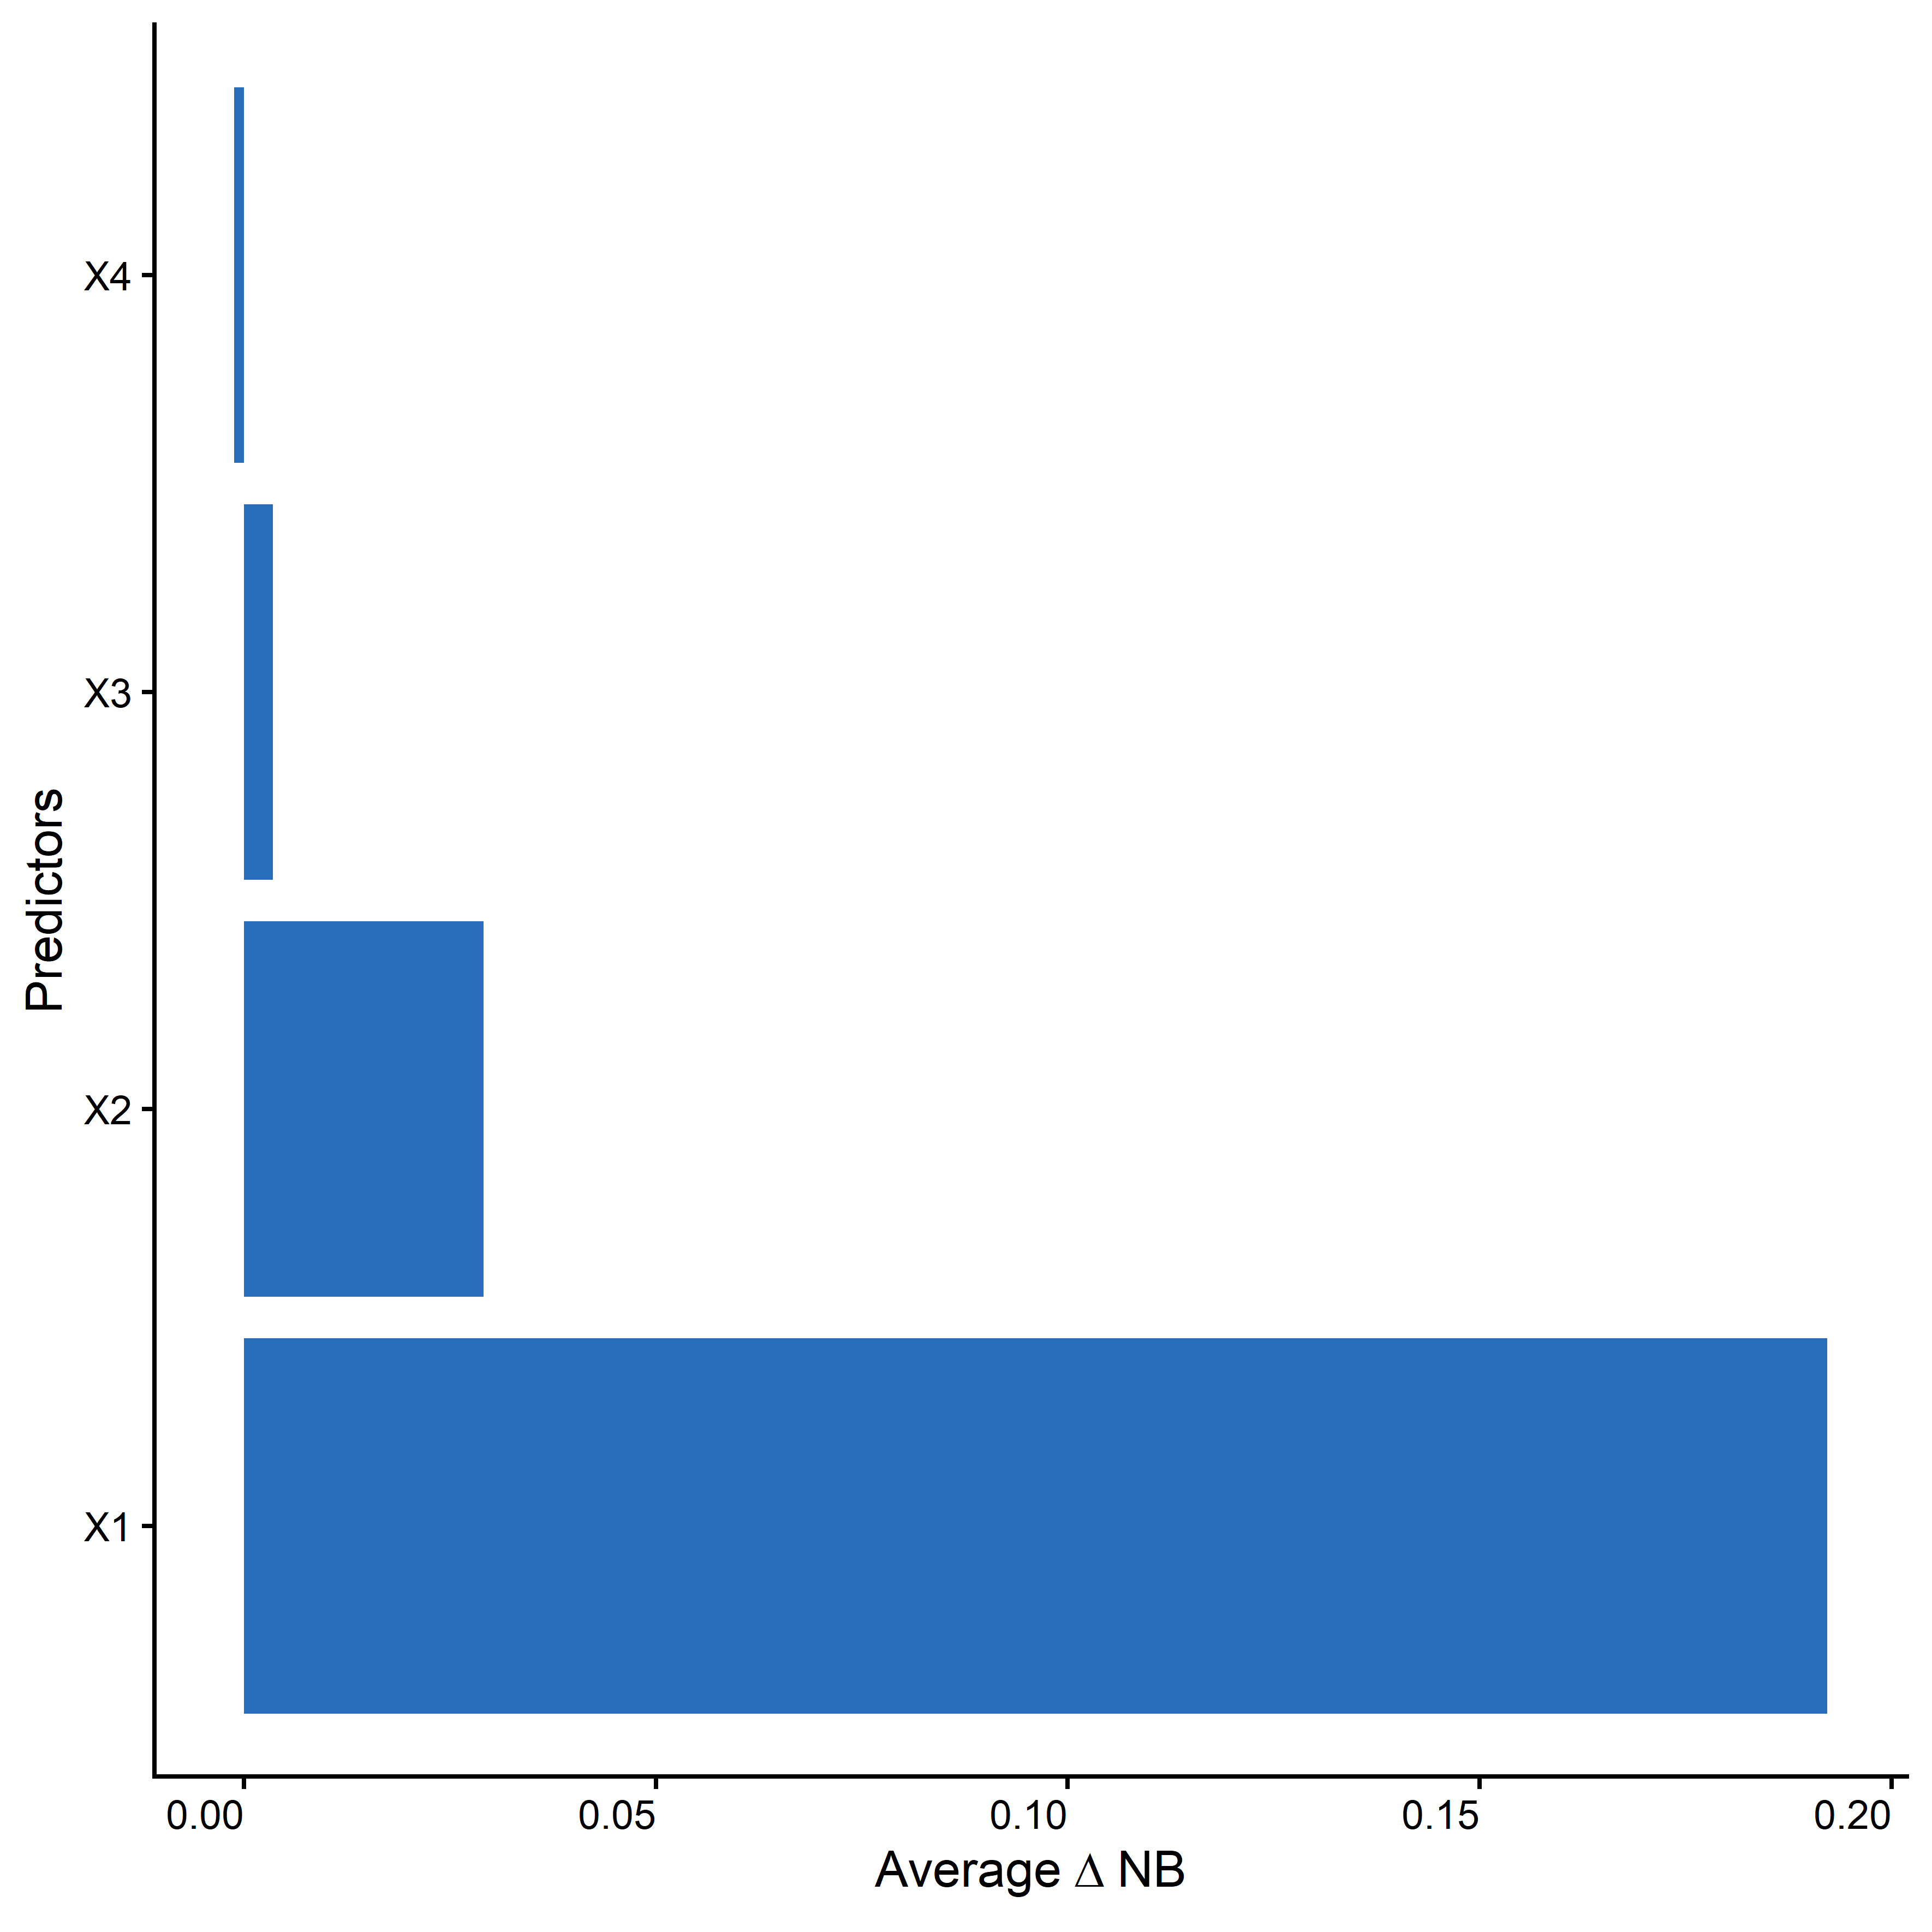
\includegraphics[width=\textwidth]{figures/varselection/fig-simple_illustration_train-1.png}
	\caption{Net benefit based variable importance for the simple illustration. NB: Net benefit.}
\end{subfigure}\hfill
\begin{subfigure}[t]{0.48\textwidth}
	\centering
	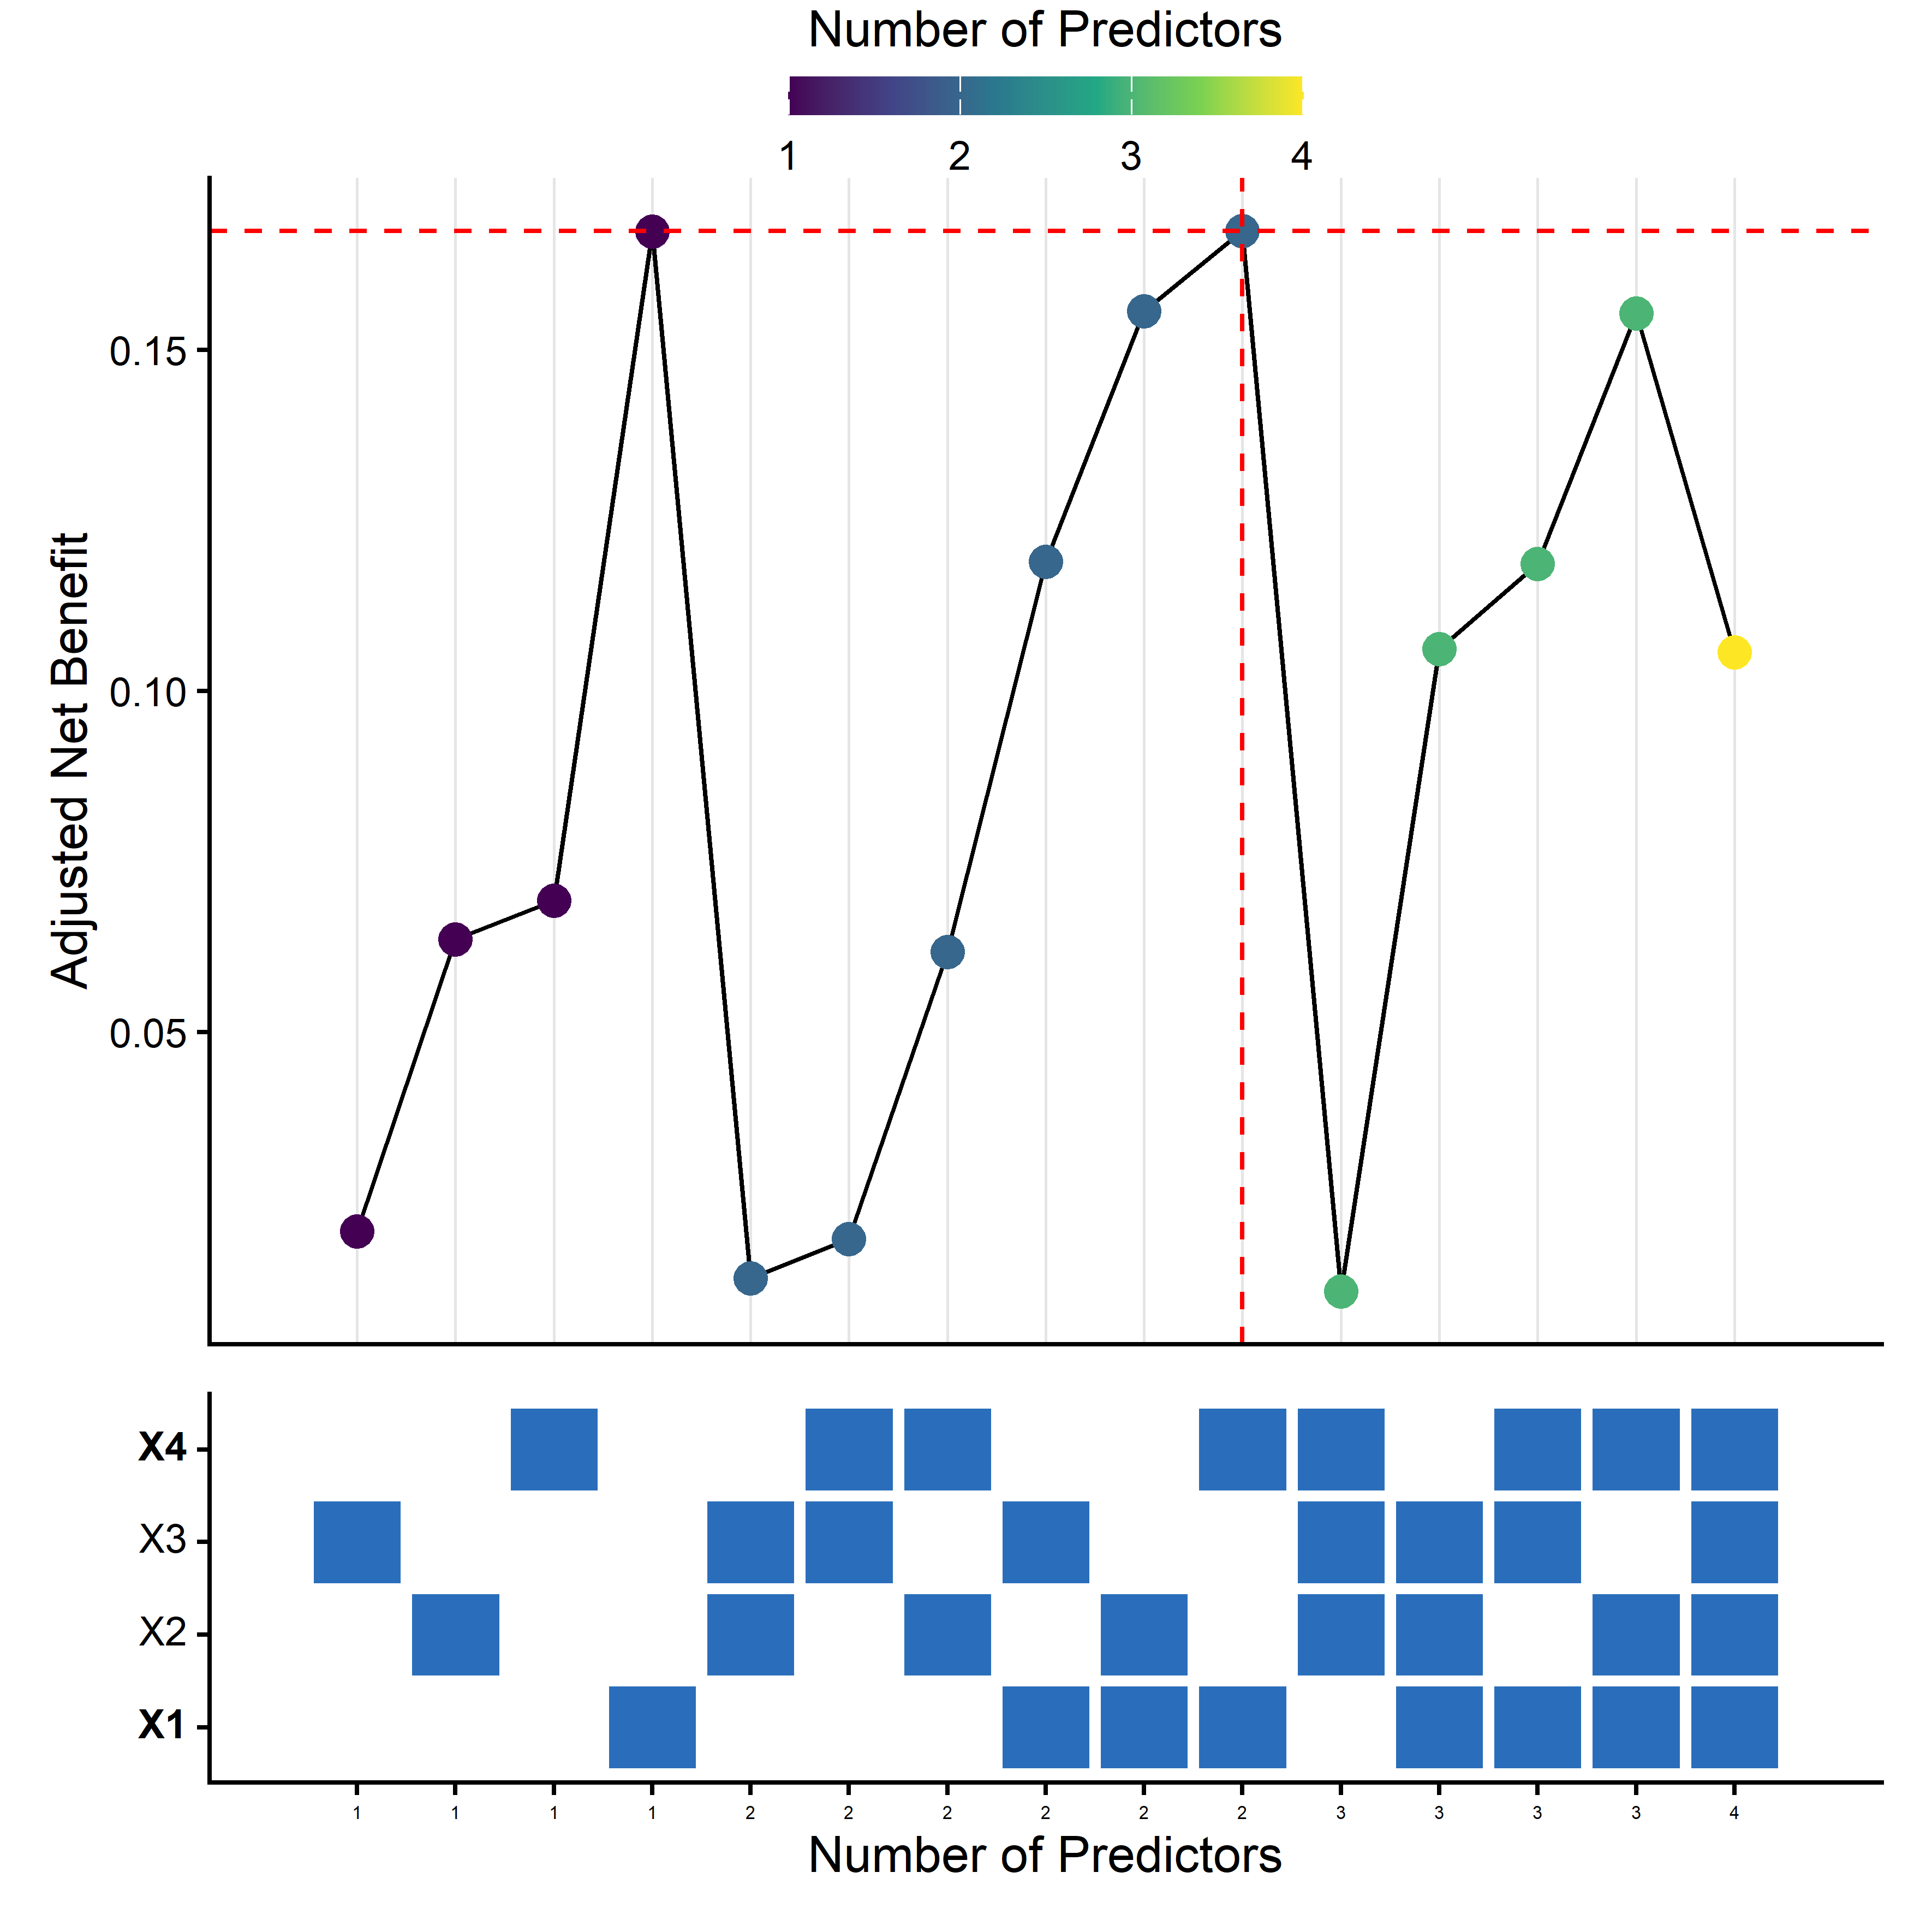
\includegraphics[width=\textwidth]{figures/varselection/fig-simple_illustration_train-2.png}
	\caption{All-subset plot for the simple illustration.}
\end{subfigure}
\label{fig:varsel:importance}
\end{figure}

This simple illustration serves as an example on how the best subset of predictors based on performance in statistical terms does not necessarily mean better cost-utility. Then, using the same data generating mechanism we generated a larger test dataset (N = 100,000) for the three possible models based on the variable selection procedure selected. Table~\ref{tab:varsel:models} presents the results of the three models in 1000 bootstrap samples. In Figure~\ref{fig:varsel:dca} we illustrate the harm adjusted decision curves (A) of the three models and flexible calibration curves (B) using restricted cubic splines as smoother. As expected, the best model according to the harm-adjusted NB is always the simpler model. The right plot illustrates that calibration for that model is slightly worse, showcasing the need to find a balance between statistical performance and decision-making.


% Placeholder for Figure 2 (Decision curve and calibration)
\begin{figure}[h!]
\centering
\begin{subfigure}[t]{0.48\textwidth}
	\centering
	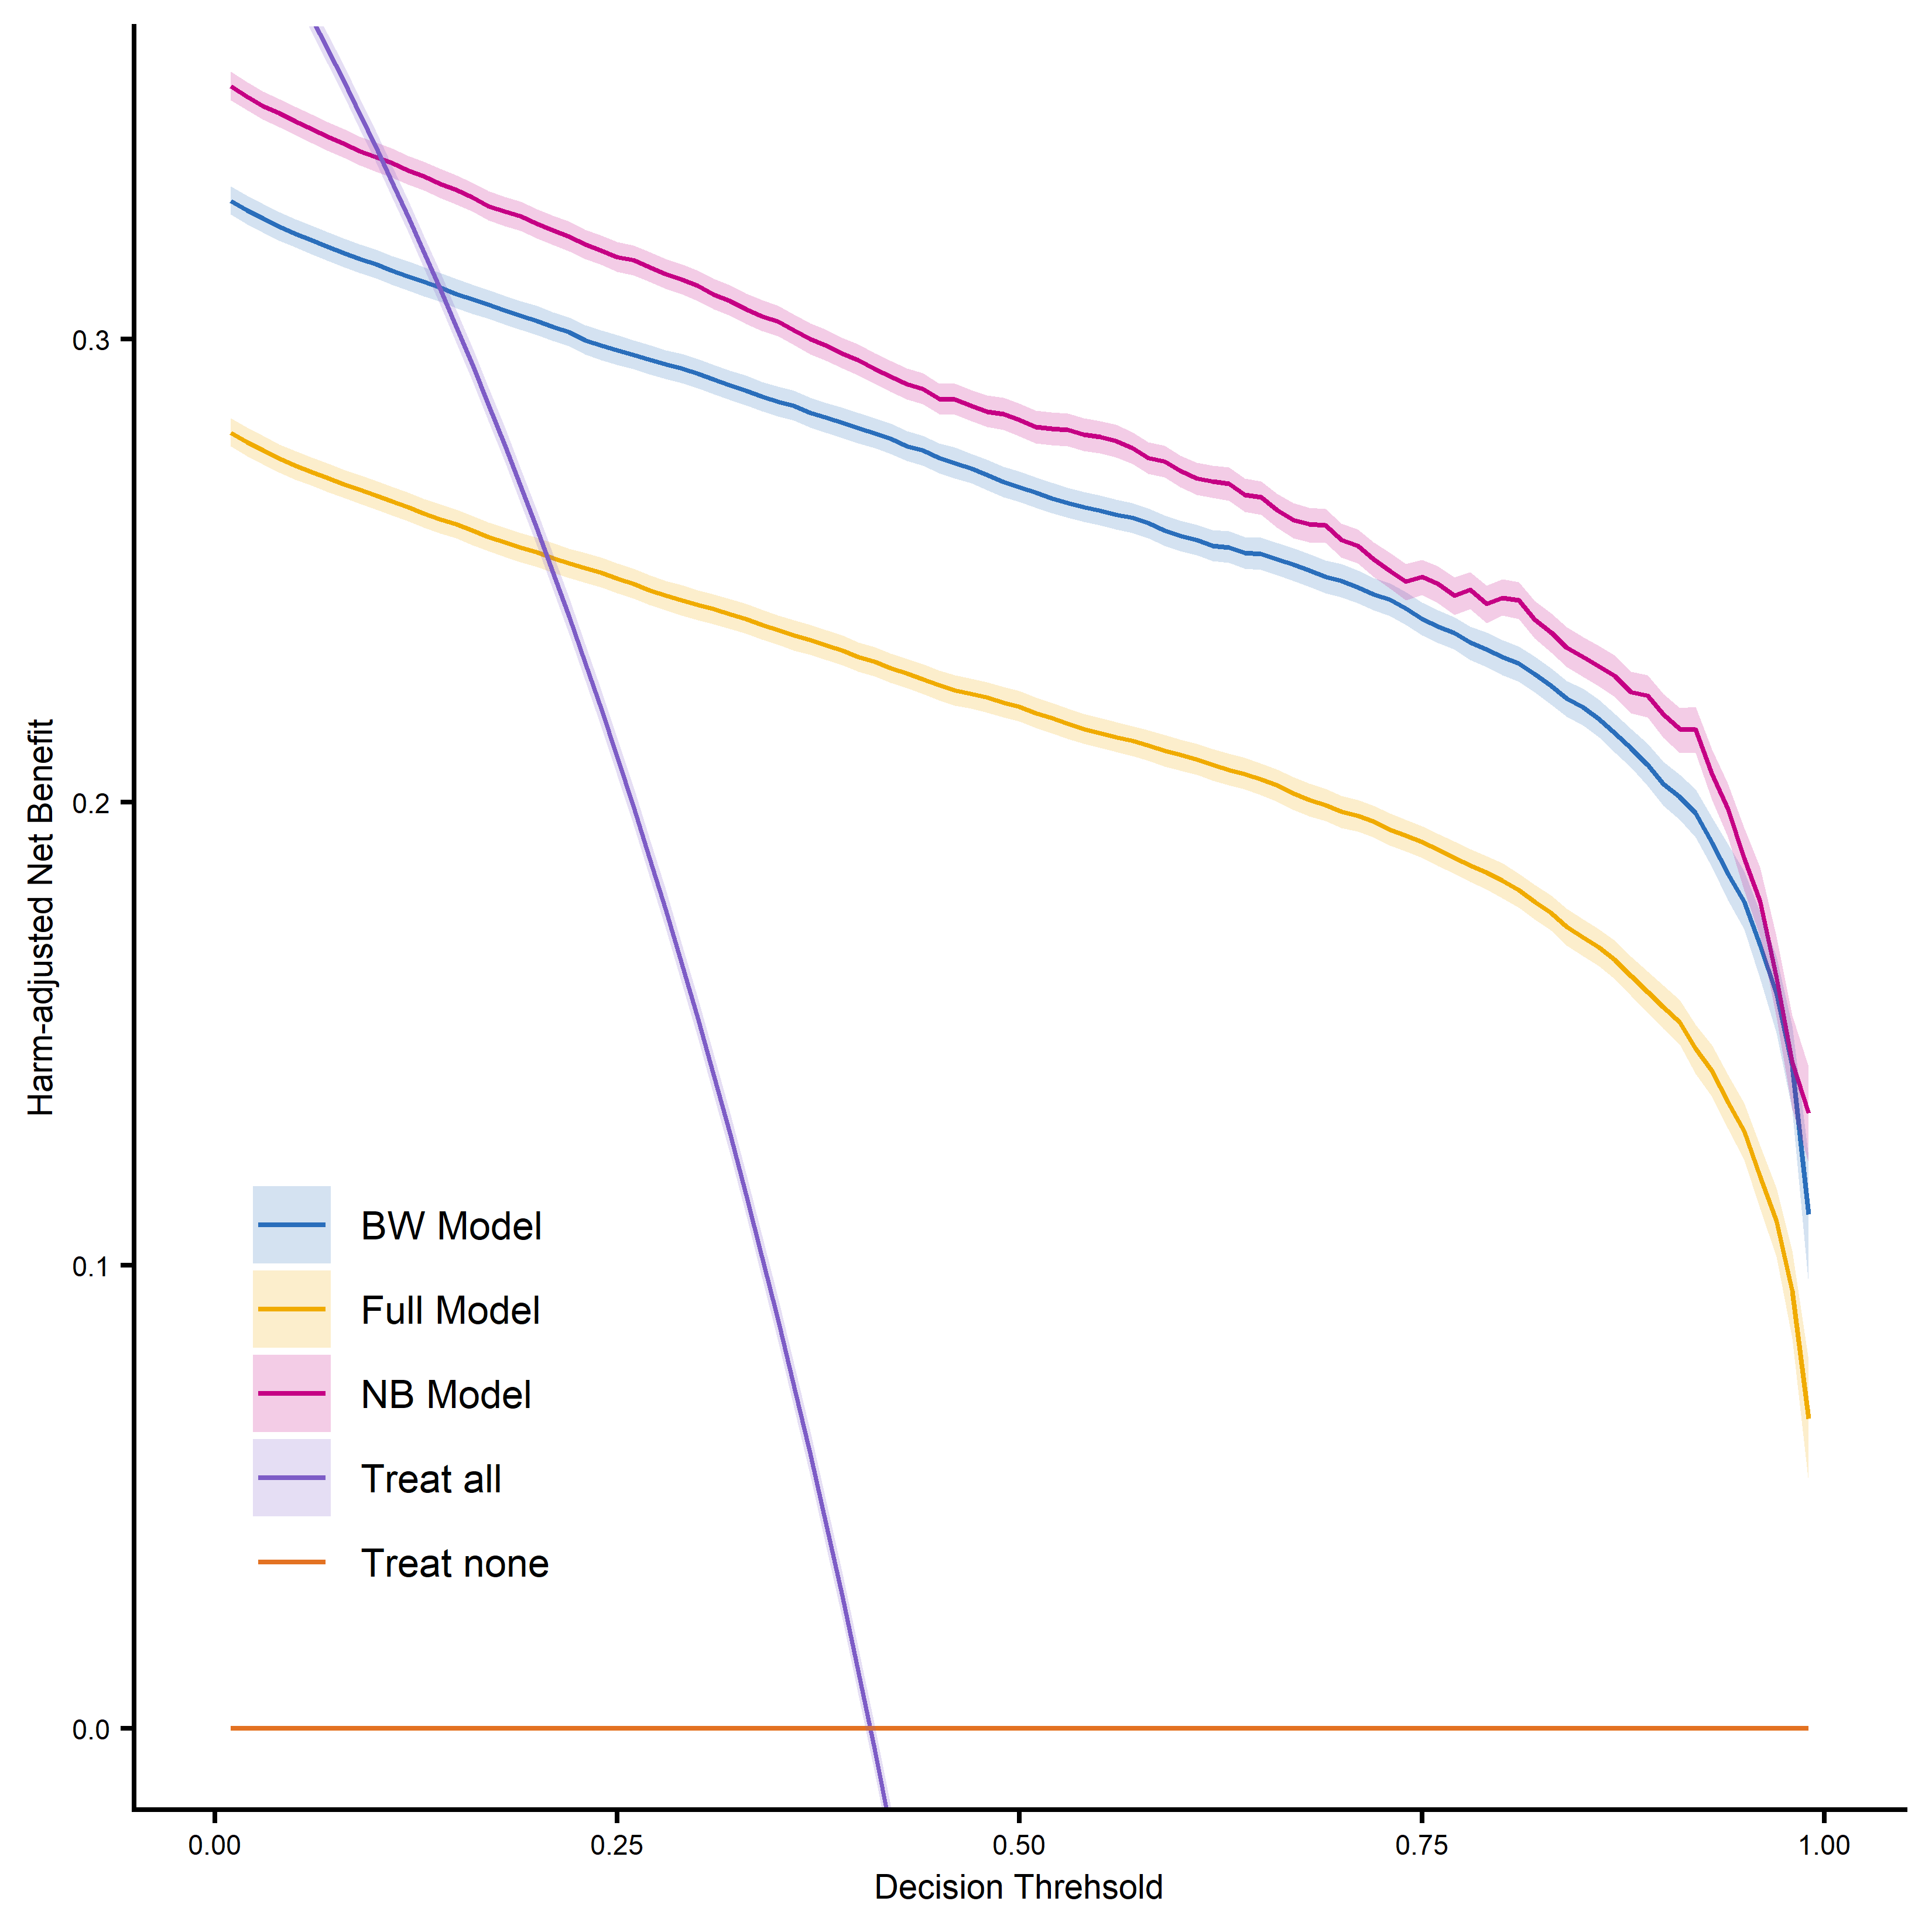
\includegraphics[width=\textwidth]{figures/varselection/fig-simple_illustration_test-1.png}
	\caption{Decision curve analysis for the simple illustration. NB: Net benefit.}
\end{subfigure}\hfill
\begin{subfigure}[t]{0.48\textwidth}
	\centering
	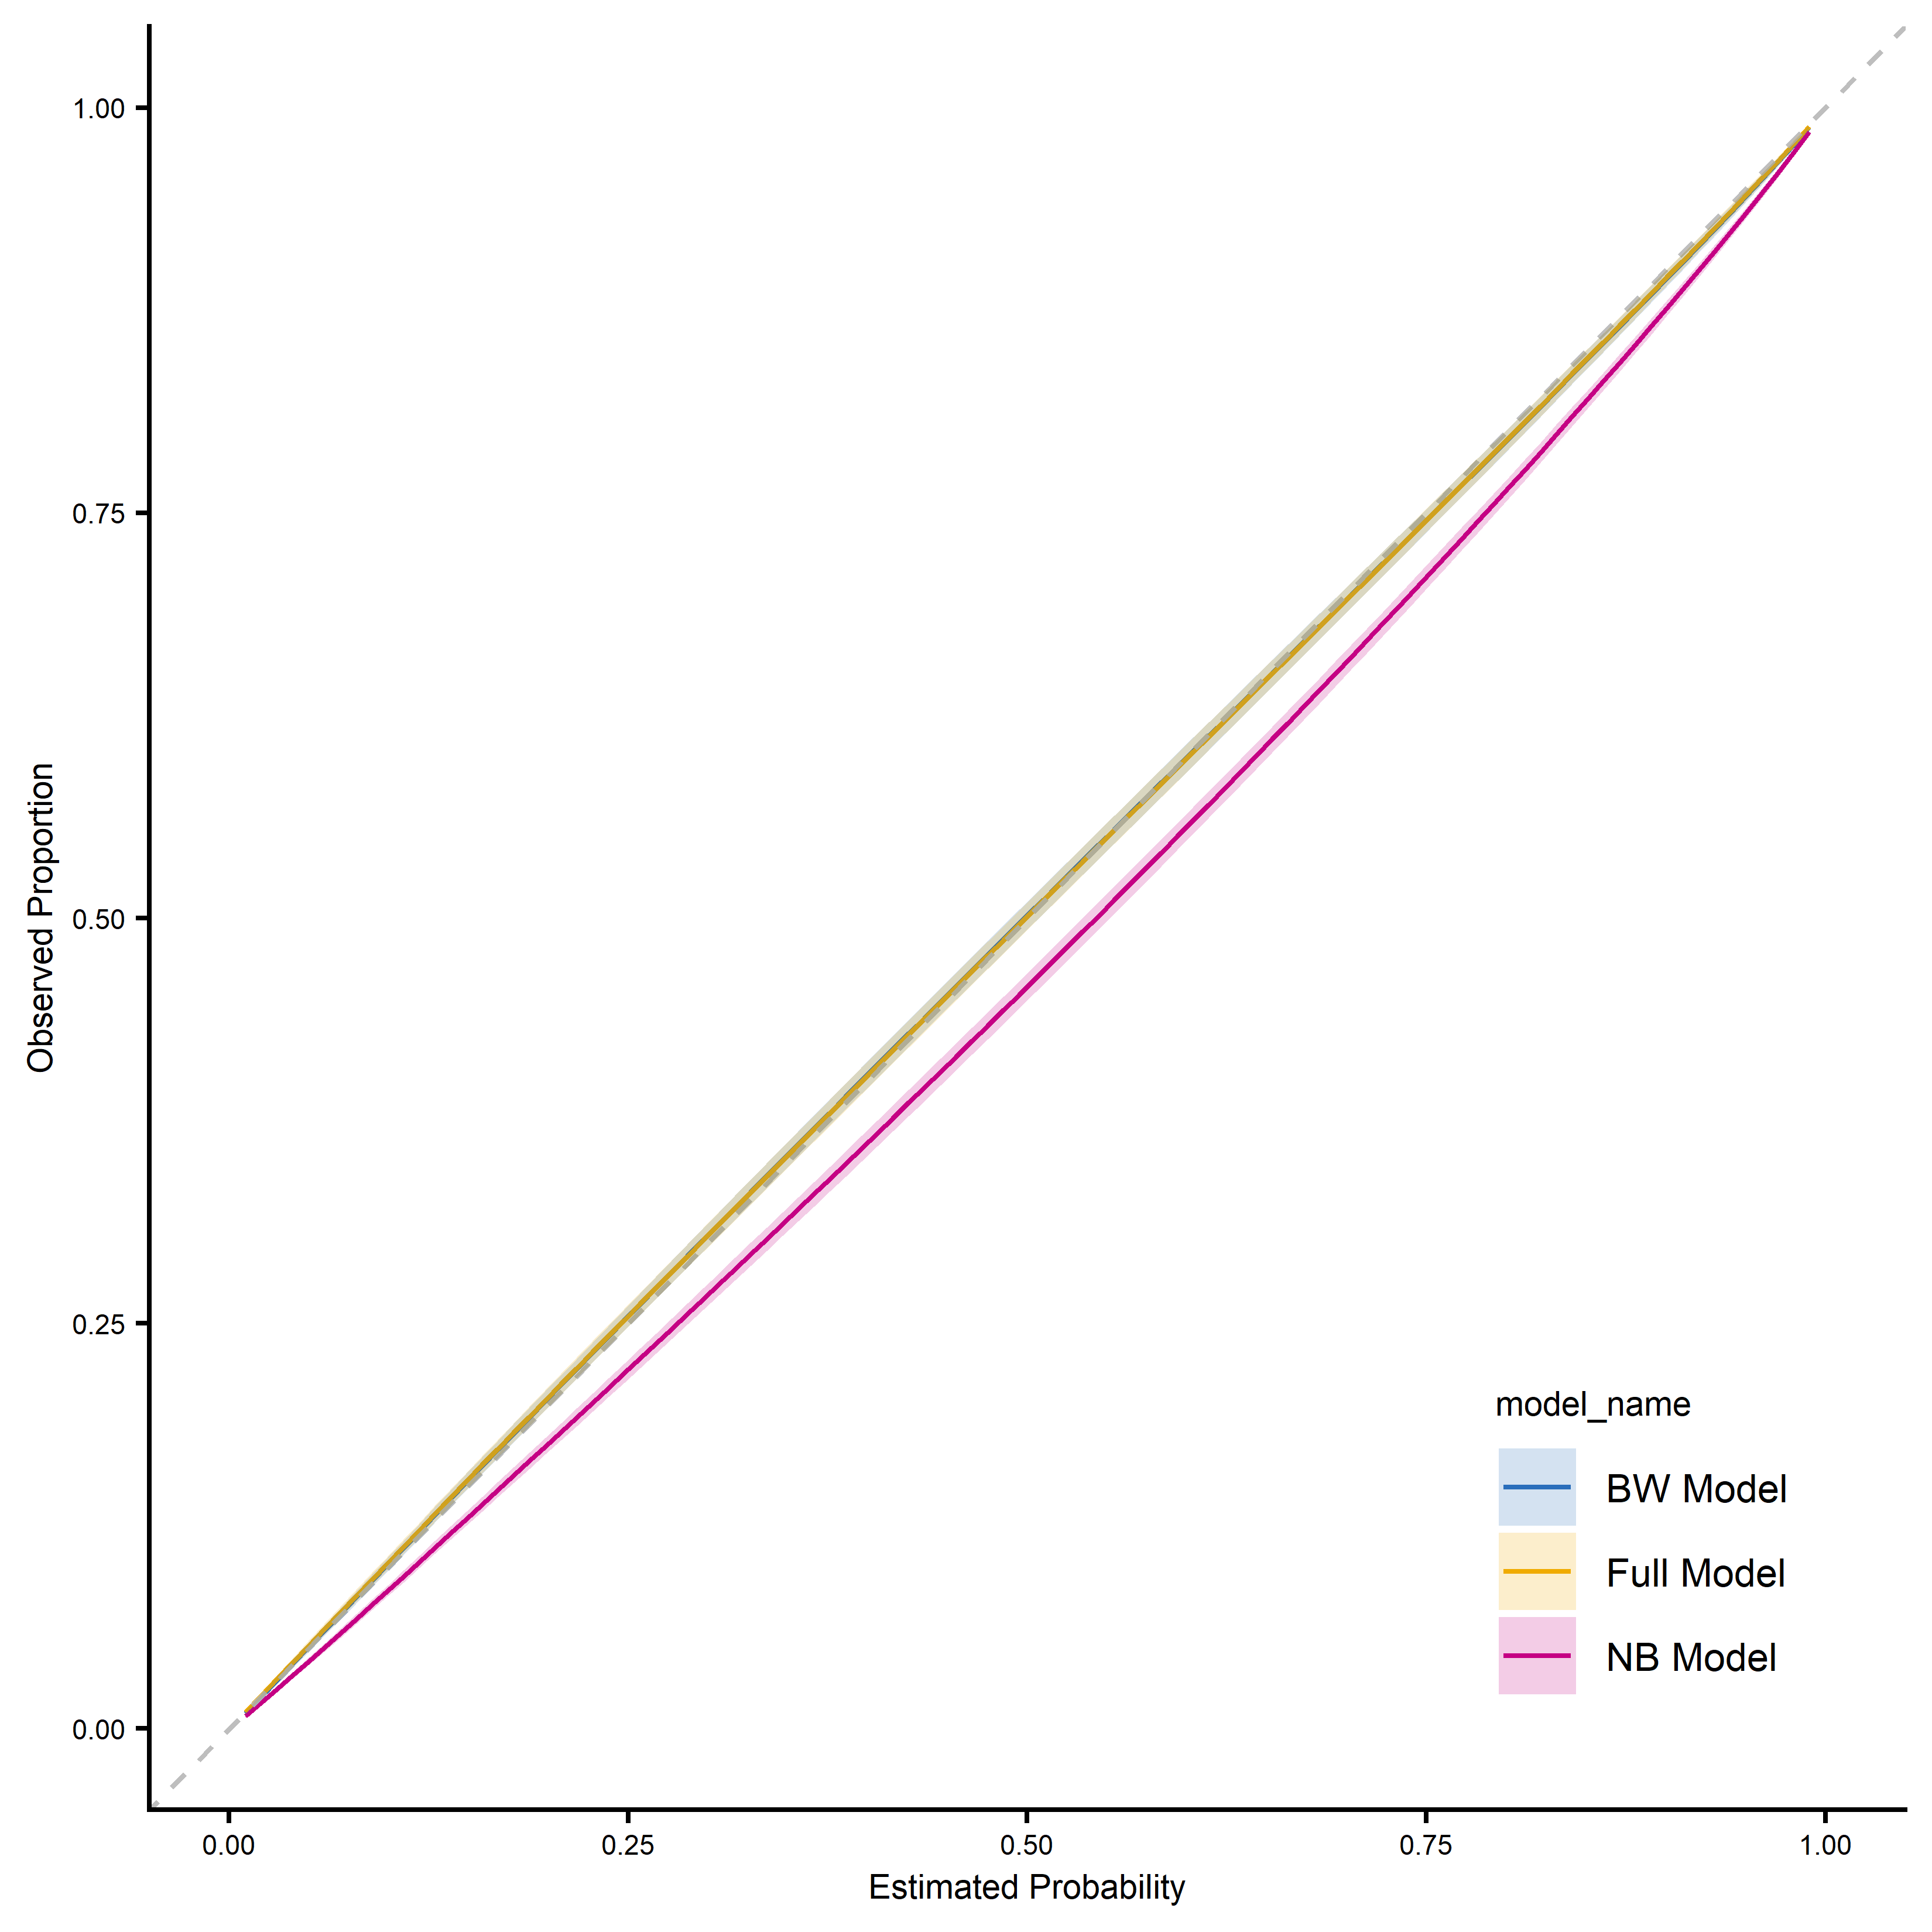
\includegraphics[width=\textwidth]{figures/varselection/fig-simple_illustration_test-2.png}
	\caption{Calibration plot for the simple illustration.}
\end{subfigure}
\label{fig:varsel:dca}
\end{figure}


\begin{table}[h!]
\centering
\small
\caption{Model comparison (mean ± 95\% CI over 1000 bootstraps on test set of 100k observations; NB threshold 10\%).}
\begin{tabularx}{\textwidth}{XXXXXXX}
\toprule
\textbf{Method} & \textbf{AUC} & \textbf{Brier} & \textbf{O:E} & \textbf{Net} & \textbf{Harm} \\
 & & & \textbf{ratio} & \textbf{Benefit} & \textbf{Adj. NB} \\
\midrule
Backward elim. & 0.970 & 0.068 & 0.987 & 0.522 & 0.371 \\
Perform. (CV) & 0.974 & 0.064 & 0.990 & 0.522 & 0.361 \\
Net Benefit & 0.966 & 0.074 & 0.974 & 0.522 & 0.421 \\
\bottomrule
\end{tabularx}
\label{tab:varsel:models}
\end{table}

\section{Case studies}

We will test the variable selection methodology with three datasets previously used to develop clinical prediction models. We will then compare the performance in terms of discrimination (AUC), calibration (calibration plots) and clinical utility (Net Benefit and DCA).

The analysis was performed on an HP EliteDesk 8 Tower G11 Desktop AI PC equipped with an Intel Core Ultra 9 285 processor (24 cores, base frequency 2.50 GHz) and 128 GB of RAM, running on a 64-bit Windows operating system and with R version 4.4. The parallelized processes used 23 cores.

\subsection{Ovarian cancer diagnosis -- IOTA data}

The optimal management of patients with an ovarian tumour depends on the histology of the mass. Benign masses do not always need to be removed and can be monitored with ultrasound follow up  \cite{carleyLaparoscopyLaparotomyManagement2002}. According to a recent study with 2 year follow-up, most of these masses spontaneously resolve, which reduces the risk of surgical complications  \cite{froymanRiskComplicationsPatients2019}. If the mass is malignant, management in specialised oncology centers is suggested \cite{timmermanESGOISUOGIOTA2021}. The IOTA group has developed and implemented several prediction models that use ultrasound and clinical characteristics to estimate the risk of malignancy of ovarian masses preoperatively  \cite{kaijserImprovingStrategiesDiagnosing2013}. In 2014, the ADNEX model was published using data from the IOTA phases 1-3 (N = 5909) Van Calster et al. (2014) \cite{vancalsterEvaluatingRiskOvarian2014}. The model has shown excellent performance across different settings and populations, as shown in recent systematic reviews and meta-analyses \cite{bbarrenadaADNEXRiskPrediction2024,barrenadaHeadHeadComparison2025}. ADNEX is a multinomial model that predicts the risk of benign, borderline, stage I invasive cancer, stage II-IV invasive cancer or metastatic cancer. In this work, we will treat it as a binary model, where the risk of malignancy is equal to the sum of the four malignant subtypes. As a validation dataset we will use IOTA phase 5 study (N = 6847) which was prospectively collected to externally validate ADNEX  \cite{vancalsterValidationModelsDiagnose2020}.

The variable selection procedure is detailed in the supplementary material of the original publication \cite{vancalsterEvaluatingRiskOvarian2014}, we refer the reader there for details. The original ADNEX model utilized nine predictors: three clinical (age, serum CA125, and center type) and six ultrasound-based (lesion diameter, solid tissue proportion, >10 cyst locules, number of papillary projections, acoustic shadows, and ascites). While family history was initially considered, it was excluded during the variable selection process. For our analysis, missing CA125 values were handled via a regression-based imputation using all other ADNEX predictors, following recent methodological recommendations \cite{siskImputationMissingIndicators2023}. Then this model was applied to the development and validation dataset to impute missing values. In the validation dataset, some of the tumours were classified as uncertain for various reasons. In the published validation study, these values were also imputed with multiple imputation. We use those imputed values for our analysis.

We extended the original predictor set with five additional features: bilateral masses, irregular internal cyst walls, Doppler color score, maximum solid component diameter, and lesion-associated pain. In total 65,536 predictor combinations were evaluated across decision thresholds from 1\% to 20\% risk with 20-fold cross validation. We then compute discrimination in terms of AUC, clustered calibration and decision curve analysis \cite{barrenadaClusteredFlexibleCalibration2026}. Adjusted NB was also calculated with costs based on three group of variables: clinical history variables (no cost, should be available for all patients from the records), ultrasound based variables (TT = 200), blood based variables (TT = 80). We compared NB based variables selections to LASSO and backward elimination. The total time to run the algorithm was 1h 25 minutes.

All models removed family history of ovarian cancer. The LASSO model also removed presence of papillary projections. NB based models removed instead maximum diameter of the solid part of the tumour and in addition the adjusted NB removed CA125 biomarker. According to the variable importance calculations, the least important predictor was family history and the most important one was the proportion of solid tissue.

The models showed comparable performance, with BE and NB-based approaches outperforming slightly the rest. Clinical utility of all models was similar, as shown in the decision curves, but when the costs of measuring a predictor are accounted for, the variable selection with adjusted NB was clearly more useful across the whole range of decision thresholds.

% Placeholder for Table showing IOTA results
\begin{table}[h!]
\centering
\small
\caption{IOTA variable selection comparison (VS = procedure, BE = backward elimination, Fam hist = family history, Pap = papillary projections, MSD = max solid diameter, Adj = adjusted).}
\begin{tabularx}{\textwidth}{XXXXXX}
\toprule
\textbf{VS Procedure} & \textbf{Removed} & \textbf{AUC} & \textbf{O:E} & \textbf{NB} & \textbf{Adj} \\
 &  & & \textbf{ratio} & \textbf{(10\%)} & \textbf{NB} \\
\midrule
BE & Fam hist & 0.961 & 0.957 & 0.226 & 0.209 \\
LASSO & Fam hist, Pap & 0.953 & 0.929 & 0.223 & 0.205 \\
NB & Fam hist, MSD & 0.961 & 0.974 & 0.227 & 0.209 \\
Adj NB & Fam hist, CA125 & 0.960 & 0.968 & 0.226 & 0.219 \\
\bottomrule
\end{tabularx}
\label{tab:varsel:iota}
\end{table}

% Placeholder for DCA figure
\begin{figure}[h!]
\centering
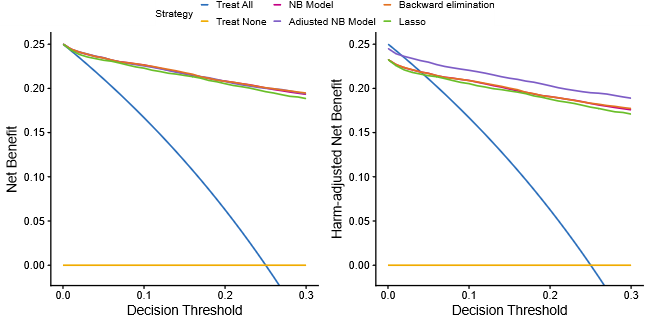
\includegraphics[width=0.8\textwidth]{figures/varselection/ADNEX_dca.png}
\caption{Decision curve analysis for unadjusted (left) and harm-adjusted (right) for the different variable selection procedures (IOTA ovarian cancer data).}
\label{fig:varsel:iota}
\end{figure}

\subsection{Emergency department hospitalization -- MIMIC IV ED (Large dimensional setting)}

For the second case study we will use the well-known MIMIC IV emergency department (MIMIC IV ED) data combined with the MIMIC IV to predict the risk of hospitalization after visiting the emergency department \cite{PhysioNet-mimiciv-3.1,hysioNet-mimic-iv-ed-2.2,johnsonMIMICIVFreelyAccessible2023}. MIMIC IV ED contains electronic health records data collected retrospectively from more than 425,000 emergency department stays in the Beth Israel Deaconess Medical Center in Boston, between 2011 and 2019. We use the benchmark proposed by Xie et al., but with the latest version of MIMIC IV (v3.1) and MIMIC ED (v2.2) Xie et al. (2022) \cite{xieBenchmarkingEmergencyDepartment2022}. The authors propose this benchmark to allow different model developers to make fair comparisons when using MIMIC IV data, therefore we followed the same procedure to obtain the training and test data according to their guidelines. The training data contains 334,420 (80\%) patients and the testing data 83605 (20\%).

They propose 64 predictors to develop models to predict risk of hospitalization when a patient arrives to the emergency department, and they develop models using different algorithms, but we will focus on the LR model, that we denote as baseline model. The predictor distribution across test and training datasets is identical and is displayed in Table S6. If we were to use the exhaustive approach as in the ovarian cancer case this would mean approximately $2^{64}$ (million trillion) combinations, which obviously is not feasible. Therefore we will use the groupwise approach with group sizes 1 and 2.

The method with a group size of one completely ignores interactions between predictors, similar to backward elimination. In the first step, the algorithm trains 65 models, followed by 64 in the next step, and so on. For MIMIC IV-ED dataset, 8 predictors were removed using this algorithm and the process took 1.45 hours. The method with group size of two iteratively removes predictors in pairs, so it accounts for interactions of two predictors. This method is computationally more intensive because the algorithm needs to train 2017 models in first step, followed by 1953 and so on. In the data, the algorithm removed 12 predictors in 6 steps.

The most important predictors according to NB variable selection were triage acuity and age of the patient. Baseline model and groupwise approaches obtained similar AUC (0.81), but the groupwise approaches tended to obtain less extreme probabilities but consistently ranked slightly higher for clinical utility across the decision curve.

% Placeholder for Table showing MIMIC-ED results
\begin{table}[h!]
\centering
\footnotesize
\caption{MIMIC-ED variable selection comparison (Pred. = predictors, Mean NB = mean net benefit).}

\begin{tabularx}{0.6\textwidth}{XXXXX}
\toprule
\textbf{Method} & \textbf{Pred.} & \textbf{AUC} & \textbf{Time} & \textbf{Mean NB} \\
 & \textbf{Removed} & & & (20--80\%) \\
\midrule
Baseline & 0 & 0.810 & -- & 0.234 \\
Groupwise (1) & 8 & 0.811 & 1.45h & 0.241 \\
Groupwise (2) & 12 & 0.809 & 1.17d & 0.239 \\
\bottomrule
\end{tabularx}
\label{tab:varsel:mimic}
\end{table}

% Placeholder for Calibration plot
\begin{figure}[h!]
\centering
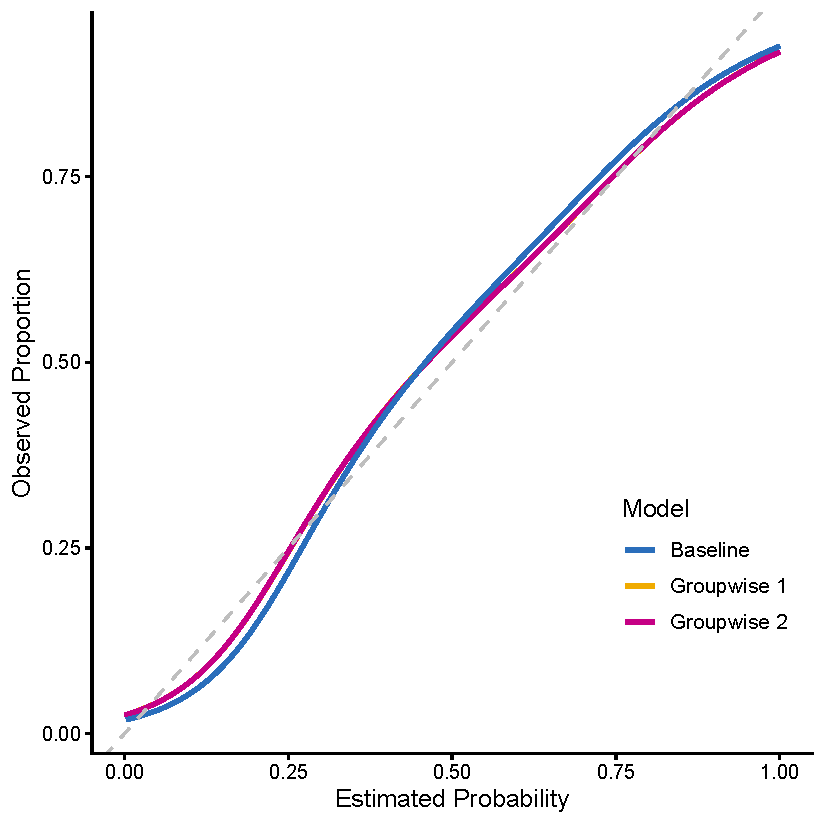
\includegraphics[width=0.8\textwidth]{figures/varselection/calibration_groupwise_mimic.pdf}
\caption{Calibration plot for the MIMIC-ED case study. Calibration for groupwise 1 and 2 are fully overlapping. (Results: Groupwise 1 time 1.458248 hours, Groupwise 2 time 1.165657 days)}
\label{fig:varsel:mimic}
\end{figure}

\subsection{Non typhoidal Salmonella (NTS) - DeNTS trial}

The last case study will use prospective cohort data to predict the risk of non-typhoidal Salmonella (NTS) bloodstream infection in children under five to guide the choice of empirical antibiotics  \cite{tackDevelopingClinicalPrediction2025}. The dataset contains clinical information collected prospectively from 2,327 paediatric hospital admissions with severe febrile illness at the Kisantu district hospital in the Democratic Republic of Congo. We use the a priori clinical predictors proposed by Tack et al., applying their exact variable definitions and restricted cubic spline transformations for continuous predictors. The authors propose this specific set of predictors based on a systematic literature review to ensure clinical relevance and avoid data-driven bias; therefore, we followed the same procedure to obtain our variables according to their guidelines. They propose 11 predictors to develop models for antibiotic triage, and they develop a simplified clinical scoring system alongside it, but we will focus on their main multivariable logistic regression (LR) model.

In their work, variables were selected using a double backward elimination process and the final model was fitted using Firth's correction  \cite{puhrFirthsLogisticRegression2017}. We will compare their approach to the introduced net benefit variable selection including splines for continuous predictors and then fitting the final model also using Firth's correction. In our algorithm, continuous predictors were introduced either with splines or were removed. The authors propose the reasonable range of thresholds to be between 20\% and 50\% so this were the range of thresholds used in the variable selection procedure.

If we were to use the exhaustive variable selection approach as in previous case studies, this would mean evaluating exactly 2,047 combinations. No test data was available, therefore, we present apparent results first and then to correct for optimism and compare the published approach and our algorithm we repeated the process across 1000 bootstrap samples.

\subsubsection{Apparent performance}

According to NB variable selection, the model removed the age, malnutrition and hemoglobin levels. Individual risks varied considerably among the published model and the model where variables were removed. The calibration of the model was closer to the diagonal for the NB model for estimated risk below 45\% but tended to estimate too low risks in higher estimated probabilities. The model had higher NB from decision thresholds of 25\% till 55\%.

% Placeholder for Figure showing risk distribution
\begin{figure}[h!]
\centering
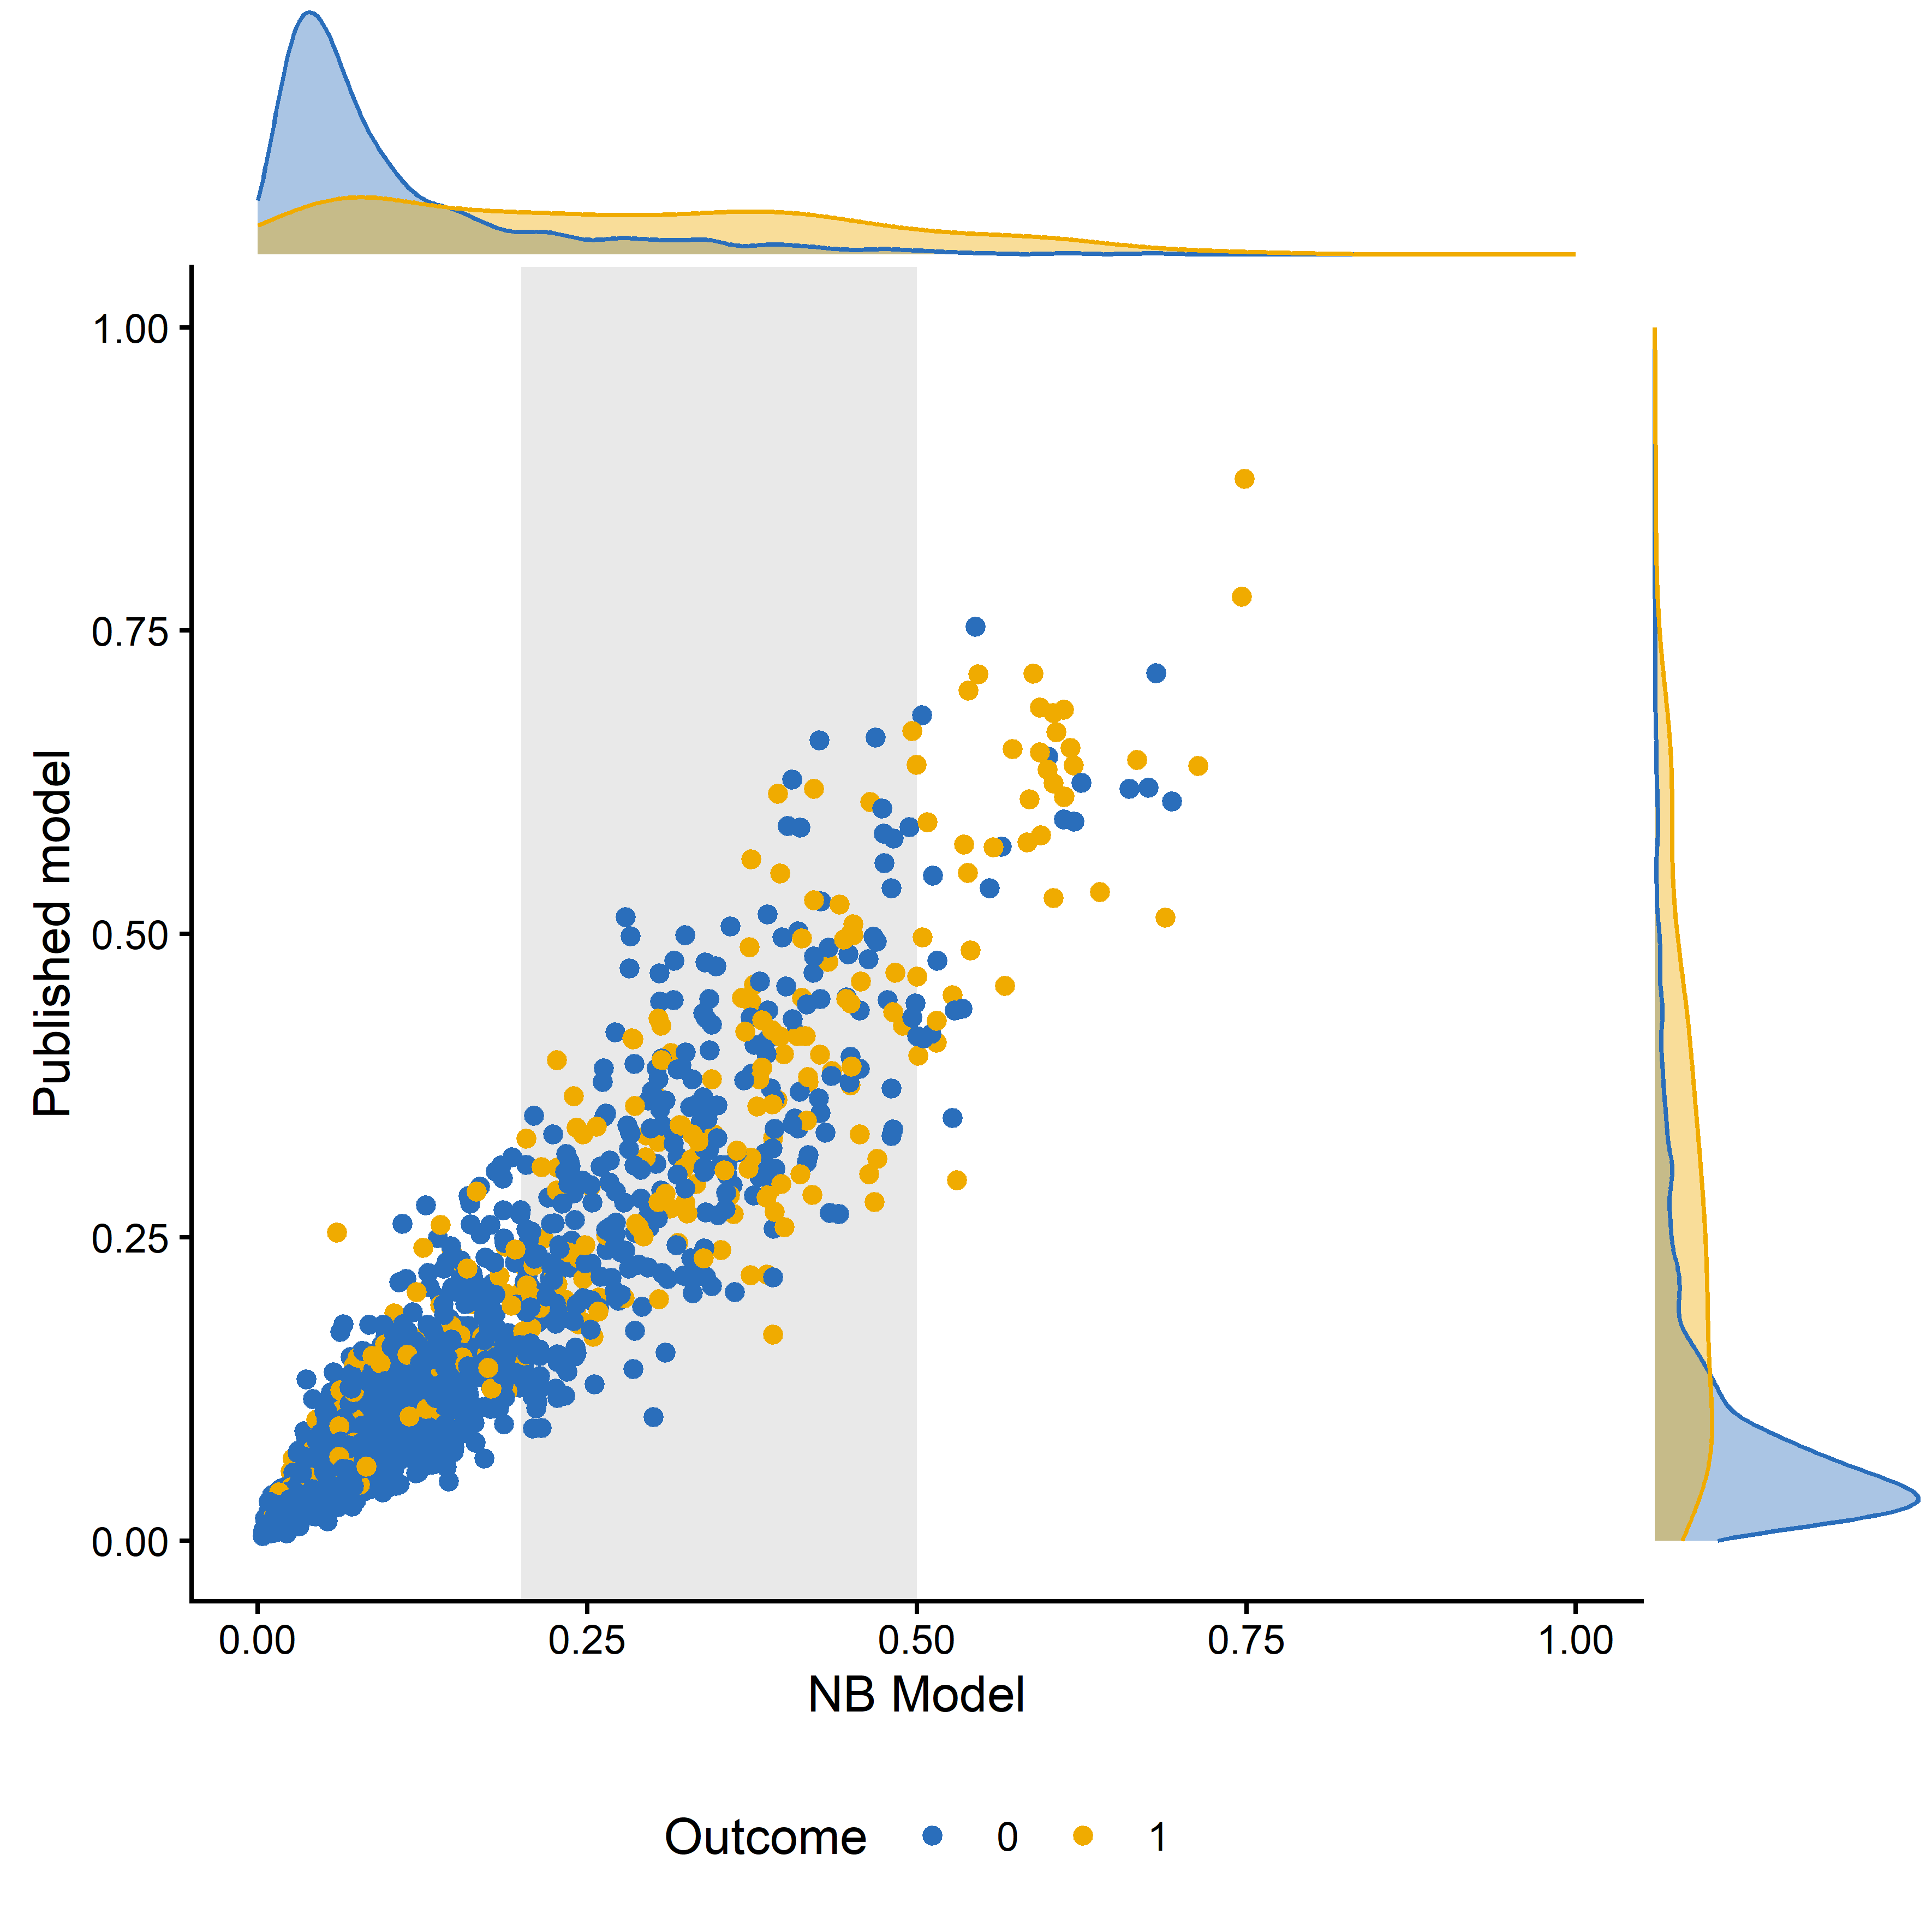
\includegraphics[width=0.8\textwidth]{figures/varselection/fig-auc_dents-1.png}
\caption{Distribution of individual risks for the model based on NB variable selection and the published model by outcome. Plots in the margin depict densities per outcome.}
\label{fig:varsel:dents}
\end{figure}

\subsubsection{Bootstrap results}

Discrimination and calibration metrics showed similar results for both models. However, the median net benefit across the reasonable range of decision thresholds was better for the NB based variable selection algorithm.

% Placeholder for Table showing DeNTS results
\begin{table}[h!]
\centering
\footnotesize
\begin{tabular}{lccc}
\toprule
\textbf{Metric} & \textbf{Published} & \textbf{NB} & \textbf{Diff} \\
 & \textbf{Model} & \textbf{Selection} & \\
\midrule
AUC & 0.784 & 0.791 & +0.007 \\
Calib. O:E & 0.991 & 0.995 & +0.004 \\
Mean NB & 0.156 & 0.167 & +0.011 \\
\bottomrule
\end{tabular}
\caption{DeNTS trial results (median Q1--Q3) across 1000 bootstrap runs; AUC = AUROC, Calib = calibration, NB = net benefit, Diff = difference.}
\label{tab:varsel:dents}
\end{table}

% Placeholder for optimism-corrected DCA figure
\begin{figure}[h!]
\centering
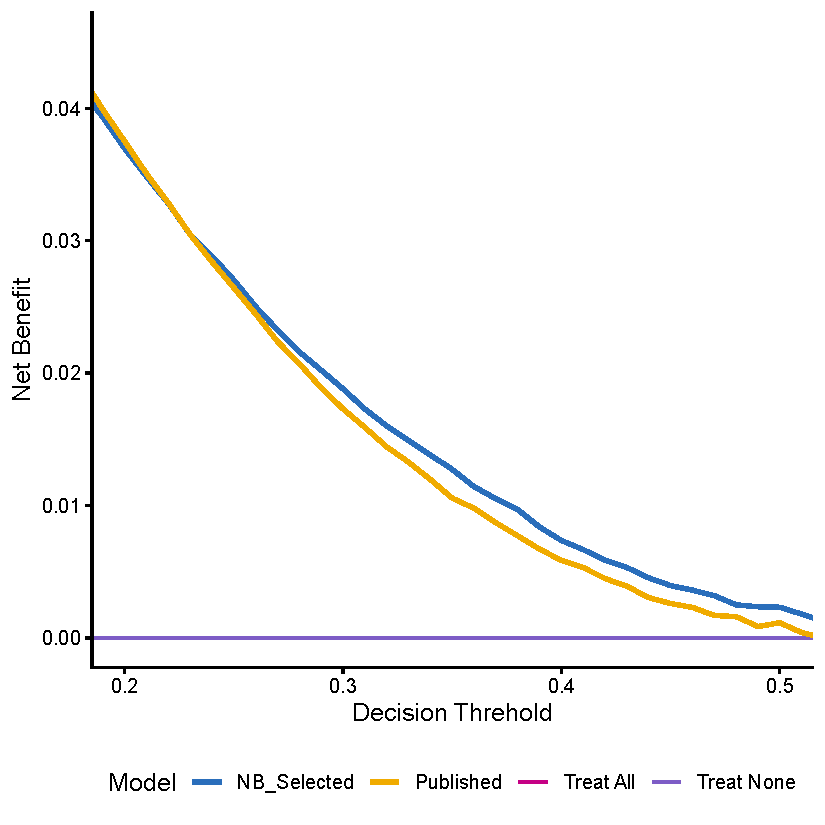
\includegraphics[width=0.8\textwidth]{figures/varselection/DCA_bootstrap_dents_zoomed.pdf}
\caption{Optimism corrected decision curve analysis based on 1000 bootstraps (Median results) for the DeNTS trial.}
\label{fig:varsel:dents_dca}
\end{figure}

\section{Discussion}

\subsection{Summary of Key Findings}

While classical statistical properties are widely used to build clinical prediction models, relying solely on them for variable selection often fails to optimise clinical benefit and to account for the real-world burden of measuring predictors. To address this gap, we developed and implemented a variable selection algorithm as an easy-to-use R package that determines the optimal subset of predictors by exhaustively exploring all predictor combinations and maximizing clinical utility, measured via (harm-adjusted) Net Benefit (NB). Through our simple illustration and three case studies, we showed that this decision analysis-based approach effectively reduces model complexity, maintaining comparable discrimination, calibration and clinical utility. In the ovarian cancer case study, adjusting for measurement harm successfully removed the CA125 biomarker, a test requiring a blood draw, while maintaining comparable performance to traditional backward elimination and LASSO methods. Furthermore, we showed that by using a groupwise elimination approach, this methodology can be successfully scaled to high-dimensional datasets like MIMIC IV-ED, yielding slightly higher clinical utility across decision thresholds compared to baseline models.

\subsection{Interpretation of Results}

The results highlight that the ``best'' model in purely statistical terms (e.g., maximizing AUC or AIC/BIC) is not necessarily the most useful model in clinical practice. Purely statistical metrics do not have the ability to balance correctly identified cases and harms of misclassifying a patient as done through NB. In addition our approach accounts for harms of measuring predictors as an crucial layer for variable selection. For instance, in our simulated illustration, ignoring test harms led to the inclusion of predictors that offered negligible improvements in NB at a disproportionate measurement cost. By translating the clinical burden into a Test Tradeoff, the minimum number of tests a doctor is willing to perform per true positive to justify the cost, our algorithm penalizes ``expensive'' predictors. Consequently, models developed using this algorithm are naturally more parsimonious and tailored for pragmatic clinical implementation, as seen in the DeNTS trial data where the NB-based model achieved a better median net benefit in the 25\% to 55\% threshold range while requiring fewer predictors.

\subsection{Contextualization Within Existing Literature}

There is growing recognition in the field of clinical prediction modelling that traditional performance measures are insufficient to guarantee a model's clinical value \cite{steyerberg2019clinical,calsterPerformanceEvaluationPredictive2024}. However, embedding utility directly into the variable selection phase has historically been difficult. While Baker et al. (2012) \cite{bakerEvaluatingNewMarker2012} discussed the use of Net Benefit to evaluate new markers, it was not operationalized as an automated variable selection algorithm. Previous attempts to introduce cost-based selection, such as the cost-adjusted Bayesian Information Criterion (BIC) proposed by Fouskakis and colleagues \cite{fouskakisBayesianVariableSelection2009}, struggled with complexity, requiring clinicians to specify difficult cost-penalized priors. Our approach bridges this methodological gap by anchoring the penalty to Net Benefit and the Test Tradeoff, providing a much more intuitive scale for clinicians to quantify the harm-to-benefit ratio.

\subsection{Limitations}

Despite its advantages, this methodology has several limitations:

\begin{enumerate}
\item Determining the specific ``harm'' of measuring a predictor is subjective, highly context-dependent, and challenging to quantify precisely prior to model development.

\item Because the method is a data-driven variable selection process, it is susceptible to overfitting, especially in studies with limited sample sizes. The procedure must strictly adhere to modern minimum sample size recommendations to prevent overly optimistic performance.

\item The exhaustive evaluation of all predictor combinations is computationally intensive and becomes infeasible with a large number of candidate predictors, though the proposed groupwise extension mitigates this issue.

\item For the moment, we only include logistic regression, but we aim to increase to other modelling algorithms.
\end{enumerate}

\subsection{Implications}

Prediction models that require burdensome, invasive, or expensive data collection for only marginal statistical gains are rarely adopted in routine care \cite{wyattCommentaryPrognosticModels1995}. By integrating clinical utility directly into the model training pipeline, developers can ensure that their final models are both statistically rigorous and practically viable. The open-source NBvarsel R package (\url{https://lasaibarrenada.github.io/NB_varsel/}) and its associated visualizations provide researchers with accessible tools to make informed, utility-driven decisions about variable selection.

\subsection{Future Research}

Future research should focus on extensive evaluation of the methodology under controlled setting with simulation studies and to extend the methodology to other modelling algorithms. For logistic regression, the methodology would also benefit of further utilities such as full control over variable interactions and spline terms. The package is intended to be continuously updated, and we made it open-source welcoming contributions from the community.

Another approach to account for clinical utility directly into parameter estimation could be using harm-adjusted NB as the optimization criterion for a loss function in deep learning architectures \cite{vickersHypothesisNetBenefit2025}.

\subsection{Conclusion}

Clinical utility should not be an afterthought reserved only for external validation. By integrating a harm-adjusted Net Benefit metric directly into the variable selection process, researchers can produce prediction models that maximize patient benefit while minimizing unnecessary clinical burden.

\glsunset{NB}
\glsunset{AUC}
\glsunset{BIC}
\glsunset{DCA}
\glsunset{TT}
\glsunset{EPV}
\glsunset{EPP}


\part{Discussion and conclusion}
\label{part:discussion}

\chapter{Discussion}
\label{ch:discussion}
\glsunset{ADNEX}
\glsunset{RMI}
\glsunset{IOTA}
\glsunset{AUC}
\glsunset{EIDM}
\glsunset{IPD}
\glsunset{SaMD}
\glsunset{MDR}
\glsunset{TRIPOD}
\glsunset{PROBAST}


This thesis set out to improve evidence-informed decision-making in the diagnosis of ovarian cancer by evaluating the \gls{ADNEX} model and advancing statistical methodology for clinical prediction models. The work integrates an applied arm --- focused on evaluating, comparing and updating \gls{ADNEX} in diverse clinical settings --- with a methodological arm that advances methodology in model development, evaluation and probability estimation. 

\section{Summary of findings}

Chapter~\ref{sec:chp_ADNEXSR} presented the first comprehensive systematic review and meta-analysis of \gls{ADNEX} external validation studies. Across 47 studies encompassing more than 17\,000 tumours, the model demonstrated robust discriminative performance, with a summary \gls{AUC} of 0.93 for distinguishing benign from malignant masses \cite{barrenadaADNEXRiskPrediction2024}. However, the review also exposed important weaknesses in the validation literature: 91\% of validations were at high risk of bias, primarily due to small sample sizes, inadequate handling of missing data, and incomplete performance assessment. Perhaps most critically, only 4 of 47 studies reported any form of calibration assessment, making it impossible to draw conclusions about the accuracy of \gls{ADNEX}'s predicted probabilities across settings.

Chapter~\ref{sec:chp_ADNEXvsRMI} extended this work with a head-to-head meta-analysis comparing \gls{ADNEX} to the \gls{RMI}, the most widely used alternative in clinical practice. The results were unequivocal: \gls{ADNEX} consistently outperformed \gls{RMI} in terms of discrimination (summary \gls{AUC} 0.92 vs 0.85 in operated patients) and clinical utility. The probability of \gls{ADNEX} being clinically useful in a hypothetical new centre was 96\%, compared to only 15\% for \gls{RMI} at the 10\% risk threshold \cite{barrenadaHeadHeadComparison2025}. These findings provide strong evidence that clinical guidelines should recommend \gls{ADNEX} over \gls{RMI} for the preoperative characterisation of ovarian masses \cite{sundarRiskpredictionModelsPostmenopausal2024,sundarDiagnosticTestsOvarian2026}.

A recurring theme throughout this thesis is that calibration --- the agreement between predicted probabilities and observed event rates --- remains underappreciated in the clinical prediction literature. The systematic reviews in Chapters~\ref{sec:chp_ADNEXSR} and~\ref{sec:chp_ADNEXvsRMI} showed that most validation studies of \gls{ADNEX} reported discrimination and classification but ignored calibration. That imbalance is methodologically weak and clinically risky. A model can rank patients correctly and still provide systematically wrong absolute probabilities, which can be harmful when the output is used to decide whether a woman with an adnexal mass should be referred, conservatively managed, or operated on \cite{vancalsterCalibrationRiskPrediction2015}. In the context of \gls{ADNEX} and prediction models as decision support tools, calibration and the probability estimate is not a secondary output: it is the output that informs action.

The same applied story motivates Chapter~\ref{sec:chp_ADNEX2}. The original \gls{ADNEX} development data were necessarily limited to women who underwent surgery, whereas in clinical practice the model is intended to be used to determine who to operate. We used bayesian refitting borrowing information from the original model to update \gls{ADNEX} with a larger and more representative dataset that includes non-operated patients. The goal is to produce  the \emph{ADNEX2} model that is better calibrated and more robust for use in a two-step strategy that starts with the simple benign descriptors, followed by the full model for indeterminate cases. ADNEX2 is undergoing medical device regulatory approval, and will be deployed in the near future through Gynaia Inc. (https://www.gynaia.com/) in a safe and easy to use app. 

Chapter~\ref{sec:chp_RFOverfitting} shifted attention from the applied model to the behaviour of algorithms used for probability estimation. Using both a case study in ovarian malignancy prediction and simulation experiments, the chapter showed that random forests can achieve almost perfect training \gls{AUC}s, which is often a sign of overfitting, and at the same time competitive test performance. The key issue is not classical overfitting in the narrow sense, but the tendency of fully grown trees to create local probability peaks and unstable risk estimates. That distinction matters because prediction models are often tuned as if classification performance were the only objective. For risk prediction, however, the quality of the probabilities themselves is central, and the default strategy of growing trees as deep as possible can be counterproductive when the goal is calibration rather than only discrimination. 

Chapter~\ref{sec:chp_ClusteredCalibration} addressed a different but closely related issue: calibration should not be treated as a purely pooled property when the data come from multiple centres. Much of the evidence used to evaluate clinical prediction models is clustered by hospital or study, yet traditional calibration plots suppress that structure. The chapter therefore proposed clustered group calibration (CG-C), two-stage meta-analysis calibration (2MA-C), and mixed model calibration (MIX-C). The main lesson is that calibration has both an overall component and a between-centre component. The recommended approaches, especially 2MA-C with splines and MIX-C, make that distinction visible by combining an overall calibration curve with prediction intervals where the calibration of a new centre should lie. That is a more realistic summary than a single pooled curve because it asks the clinically relevant question of whether a model remains well calibrated when it is moved to a new setting.

Chapter~\ref{sec:chp_FundamentalProblem} took a step back from the technical evaluation of model performance to examine a more fundamental question: how much can we trust a risk estimate for an individual patient? The study demonstrated that individual risk estimates are far more uncertain than commonly assumed. While estimation uncertainty (due to finite sample size) decreases with larger training samples, model uncertainty (due to arbitrary modelling choices) and applicability uncertainty (due to differences in measurement procedures and populations) remain substantial. Even with 10\,000 training observations, the 95\% range of predicted probabilities for the same patient averaged 0.39 on the probability scale. These findings challenge the common practice of presenting a single risk estimate to patients and clinicians without acknowledging the underlying uncertainty.

Chapter~\ref{sec:chp_varselection} is still under development, but it follows naturally from the methodological chapters. If a model is judged not only by fit but also by usefulness, then predictor selection should account for the clinical consequences of including or excluding variables. That question is especially relevant in settings such as ovarian mass diagnosis, where a model may guide referral, surgery, or follow-up decisions.



\section{Embracing uncertainty in individualised decision-making}

Clinical prediction models are developed and evaluated at the population level, but their purpose is to inform decisions for individual patients \cite{steyerbergClinicalPredictionModels2009}. The chapters in this thesis show that moving from population performance to individual decision-making adds successive layers of uncertainty. Chapter~\ref{sec:chp_ADNEXSR} established that \gls{ADNEX} performs well on average across settings. Chapter~\ref{sec:chp_ADNEXvsRMI} showed that it compares favourably with \gls{RMI} for triage. Chapter~\ref{sec:chp_ClusteredCalibration} showed that pooled performance can mask meaningful centre-to-centre variation. Chapter~\ref{sec:chp_FundamentalProblem} then showed that uncertainty persists even after all of those population-level summaries are taken into account.

That sequence matters because the apparent precision of a risk estimate can be misleading. A patient and clinician may see one number, but that number is the product of a model that may behave differently in another centre, another patient subgroup, or another data collection context. Chapter~\ref{sec:chp_ClusteredCalibration} makes this visible at the centre level; Chapter~\ref{sec:chp_FundamentalProblem} makes it visible at the individual level. 
Chapters~\ref{sec:chp_ADNEXSR} and~\ref{sec:chp_ADNEXvsRMI} established that \gls{ADNEX} performs well on average across diverse populations. However, both chapters noted considerable heterogeneity in performance across centres and studies. Chapter~\ref{sec:chp_ClusteredCalibration} provided formal methods to quantify this heterogeneity, showing that calibration can vary substantially between clusters even when the overall curve appears satisfactory. 
This has direct implications for the concept of \gls{EIDM} introduced earlier in the thesis. A predicted probability should be treated as an estimate based on the used model, not as an exact measurement. Confidence intervals will represent how uncertain the model is based on the used data, but do not guarantee that the true underliying risk of the patient lies within the interval. In practice, that means risk estimates should be communicated together with an explanation of what is known, what is uncertain, and why the estimate may change if the patient were seen in another centre or assessed under slightly different assumptions \cite{pateUncertaintyUsingRisk2019, rileyUncertaintyRiskEstimates2025, aldermanTacklingAlgorithmicBias2025, ganapathiTacklingBiasAI2022}.
Chapter~\ref{sec:chp_FundamentalProblem} pushed this line of reasoning further, showing that even within a single centre, the predicted probability for an individual patient is subject to model and applicability uncertainty that cannot be reduced by increasing sample size alone \cite{pateUncertaintyUsingRisk2019, rileyUncertaintyRiskEstimates2025}. A risk estimate of 15\% should not be interpreted as a precise measurement but rather as a point within a range of plausible values, each of which might lead to a different clinical decision.
These findings do not diminish the value of clinical prediction models. \gls{ADNEX} remains a useful tool for ovarian mass characterisation because it shows clinical utility at population level and can support referral and management decisions. The lesson is instead that its outputs should be used with caution. Clinical prediction models should support shared decision-making rather than replace it, and that requires assesments embracing this uncertainty \cite{moonsCriticalAppraisalData2014, steyerbergClinicalPredictionModels2009}.

\section{Towards honest and safe medical devices}

The systematic reviews in Chapters~\ref{sec:chp_ADNEXSR} and~\ref{sec:chp_ADNEXvsRMI} consistently identified poor methodological quality in external validation studies. This is very concerning because this evidence is of utmost importance for safe implementation of clinical prediction models \cite{steyerbergPredictionModelsNeed2016}.  The most common issues --- assessed using the \gls{PROBAST} tool \cite{wolffPROBASTToolAssess2019} --- were inadequate sample sizes, inappropriate exclusion of patients with missing data, and incomplete reporting of model performance. Adherence to the \gls{TRIPOD} reporting guidelines \cite{collinsTRIPODAIStatementUpdated2024} was low, with key items such as sample size justification, missing data handling, and calibration assessment reported in fewer than 8\% of studies. These findings are consistent with previous reviews of clinical prediction model validation studies, which have repeatedly highlighted similar issues \cite{collinsExternalValidationMultivariable2014, bouwmeesterReportingMethodsClinical2012, andaurnavarroCompletenessReportingClinical2022,andaurnavarroSystematicReviewFinds2023, andaurnavarroSystematicReviewIdentifies2023, dhimanMethodologicalConductPrognostic2022, dhimanOverinterpretationFindingsMachine2023}.

These findings are even more concerning in light of the regulatory developments discussed in the introduction. As clinical prediction models increasingly fall under medical device regulation --- including the EU \gls{MDR} and the \gls{SaMD} framework --- the evidence base for their validation must improve. Regulatory frameworks require demonstration of safety and effectiveness, which in the context of prediction models translates to robust evidence of discrimination, calibration, and clinical utility across diverse populations \cite{vancalsterPerformanceEvaluationPredictive2024, collinsTRIPODAIStatementUpdated2024}. The current state of the validation literature and regulatory approval, falls short of what should be expected for tools that are intended to be used in patients. Recent studies have highlighted that many models that have been approved and are in use, have not undergone rigorous external validation, and their performance in real-world settings is often unknown or unclear \cite{mehtaEvaluatingTransparencyAI2025,vanleeuwenArtificialIntelligenceRadiology2021}.

Improving this situation requires combined efforts from researchers and regulators. Researchers should use better study designs, with adequate sample size\cite{rileyMinimumSampleSize2021}, proper handling of missing data and prospective multicenter data collection. The quality of reporting in published literature also needs improving which can be done by adhering to international guidelines like \gls(TRIPOD) and its extensions \cite{collinsTRIPODAIStatementUpdated2024,debrayTransparentReportingMultivariable2023, snellTransparentReportingMultivariable2023}), and a shift in culture towards recognising external validation as an ongoing process rather than a one-time exercise is needed \cite{vancalsterThereNoSuch2023}. From the regulators side, there should be stricter requirements about the model's performance before approval, ensuring that at least key performance measures are presented such as the calibration plot and a clinical utility metric (i.e. Net Benefit) \cite{vancalsterPerformanceEvaluationPredictive2024, ShowUsEvidence2026}. Both perspectives are synergistic: better research leads to better evidence for regulators, and stricter regulation incentivises better research. Ultimately, the goal is to ensure that clinical prediction models are safe, effective, and trustworthy tools for improving patient care.


\section{Future directions for trustworthy AI in medicine}

There is an exponential growth in the development of clinical prediction models, but the findings of this thesis suggest that there is still much work to be done to ensure that these models are trustworthy and useful in practice. A recent systematic review showed that the probability of a new clinical prediction model being externally validated in 5 years is of 13\% \cite{arshiNumberPublicationsNew2025}. Only one in eight models will be validated, which is a requirement for being trustworthy and applied in clinical practice. The findings of this thesis suggest that there is need for more and better validation studies, with a focus on calibration and clinical utility. This is a fast growing and evolving field, and there are many opportunities for future research to improve the development, evaluation, and implementation of clinical prediction models. Some of the most promising directions include:

\subsection{Focus on clinical utility}

\subsection{Better uncertainty estimation}

\subsection{Evaluation when clustering is present}

\subsection{Policymakers and regulators as key stakeholders}

\subsection{Trustworthy AI for ovarian cancer diagnosis}

\subsection{Updating ADNEX}
The most immediate applied priority is the development and validation of \gls{ADNEX}2. The preceding chapters make clear what such an update should address: the development data should be expanded to include non-operated patients, more recent \gls{IOTA} data should be incorporated, and the updated model should be validated with methods that explicitly quantify calibration in clustered settings \cite{vancalsterEvaluatingRiskOvarian2014, steyerbergAssessmentHeterogeneityIndividual2019}. The aim is not simply to improve average performance, but to obtain a model whose probabilities remain reliable across centres and clinical contexts.

\subsection{Variable selection for clinical utility}
Current variable selection methods in prediction modelling typically optimise statistical criteria such as the Akaike Information Criterion, cross-validated log-loss, or discrimination. However, the ultimate purpose of a diagnostic prediction model is to improve clinical decisions. Developing variable selection algorithms that directly optimise for net benefit \cite{vickersNetBenefitApproaches2016} or related utility measures could lead to simpler models that are more useful in practice, even if they sacrifice a small amount of traditional statistical performance. This is the focus of the ongoing work in Chapter~\ref{sec:chp_varselection}.

\subsection{Extending clustered calibration methodology}
The methods proposed in Chapter~\ref{sec:chp_ClusteredCalibration} can be extended in several directions. Bayesian approaches to prediction interval estimation may improve coverage properties compared to the current frequentist methods. More complex heterogeneity structures, including \glspl{random_slope} and nonlinear centre effects, should be evaluated. The methods should also be tested with prediction models beyond logistic regression, including machine learning algorithms whose probability estimates may exhibit different calibration patterns.

\subsection{Uncertainty communication in clinical practice}
Chapter~\ref{sec:chp_FundamentalProblem} demonstrated that individual risk estimates carry substantial uncertainty, but translating this insight into clinical practice remains an open challenge. Future work should explore how uncertainty can be communicated effectively to clinicians and patients without undermining trust in prediction models \cite{kompaSecondOpinionNeeded2021}. Practical approaches may include prediction abstention, presenting ranges instead of point estimates, and integrating uncertainty quantification into clinical decision support systems. These developments connect directly to the broader goal of \gls{EIDM} and shared decision-making.

\subsection{Model lifecycle monitoring}
As clinical prediction models are increasingly recognised as medical devices, continuous monitoring of their performance after deployment becomes a regulatory and ethical requirement. Methods for detecting performance degradation over time --- due to changes in patient populations, clinical practice, or measurement technologies --- need to be developed and standardised. The clustered calibration methods from this thesis provide a foundation for such monitoring, but further work is needed to adapt them for sequential surveillance rather than one-time validation.



\section{Conclusion}
This thesis contributes to the development and evaluation of clinical prediction models for ovarian cancer diagnosis from both applied and methodological perspectives. The systematic evaluation of \gls{ADNEX} confirmed its value as a diagnostic tool and provided the evidence base for recommending it over alternatives such as the \gls{RMI}. At the same time, the methodological chapters showed why this should not be the end of the story: calibration is rarely assessed, probability estimates from machine learning algorithms can be misleading if not validated properly, clustering changes how performance should be interpreted, and individual risk predictions carry more uncertainty than is often acknowledged.

These findings underscore that clinical prediction models, including \gls{ADNEX}, are very valuable but they need to be used responsibly. Trustworthy AI or prediction model requires honest model development and validation, ensuring that the results are reliable and generalisable. Their responsible use requires rigorous validation, transparent communication of uncertainty, and ongoing monitoring --- principles that are increasingly formalised in both reporting guidelines and medical device regulation, although not properly enforced by some regulators \cite{,mehtaEvaluatingTransparencyAI2025}. The ongoing work on variable selection for clinical utility and the \gls{ADNEX}2 update aims to translate the methodological insights of this thesis into a better model for clinical practice.

\color{black}

 


\renewcommand*{\bibfont}{\footnotesize}
\printbibliography[heading=bibintoc]

\part{Back matter}
\label{part:backmatter}
\markboth{}{}

\chapter*{Scientific acknowledgments, personal contribution and conflict of interest statement}
\addcontentsline{toc}{chapter}{Scientific acknowledgments, personal contribution and conflict of interest statement}

\section*{Scientific acknowledgments}

...

\section*{Personal contribution}

...

\section*{Conflict of interest statement}

The authors have no conflicts of interest to declare.
\chapter*{Statement of the use of generative AI}
\addcontentsline{toc}{chapter}{Statement of the use of generative AI}

I did use generative AI assistance tools namely \textit{Gemini 3 PRO}, \textit{Github Copilot} and \textit{Claude}.
\textit{Gemini 3 PRO} was used for brainstorming ideas, improving the phrasing of sentences, checking grammar and solving programming issues or writing small pieces of code.
\textit{Github Copilot} was used to assist in writing code within RStudio. 
\textit{Claude} was used for transforming word document into LaTeX code. 
The text/code/ images in this thesis are my own (unless otherwise specified) and generative AI has only been used in accordance with the KU Leuven guidelines and appropriate references have been added. 
I have reviewed and edited the content as needed and I take full responsibility for the content of the thesis. 
\chapter*{Curriculum Vitae}
\addcontentsline{toc}{chapter}{Curriculum Vitae}

%--- Personal Info Header ---
\noindent
\textbf{Lasai Barreñada} \\
PhD researcher in clinical prediction models at KU Leuven. \\
\textit{Email:} lasai.barrenadataleb@kuleuven.be 

%--- Professional Experience ---
\section*{Professional Experience}

\noindent
\textbf{KU Leuven} \hfill 10/2022 -- Current \\
PhD Researcher in clinical prediction models (Leuven)

\vspace{0.5em} \noindent
\textbf{Memorial Sloan Kettering Cancer Center} \hfill 02/2025 -- 06/2025 \\
Visiting PhD Researcher (New York)

\vspace{0.5em} \noindent
\textbf{Julius center - UMC Utrecht} \hfill 10/2024 -- 02/2025 \\
Visiting PhD Researcher (Utrecht)

\vspace{0.5em} \noindent
\textbf{Basque Center for Applied Mathematics (BCAM)} \hfill 12/2021 -- 09/2022 \\
Research Technician in Machine Learning (Bilbao)

\vspace{0.5em} \noindent
\textbf{Spanish National Statistical Office (INE Spain)} \hfill 10/2020 -- 09/2021 \\
Postgraduate Internship (Madrid)

%--- Education ---
\section*{Education}

\noindent
\textbf{KU Leuven} \hfill 2022 -- 2026 (expected) \\
PhD in Biomedical Sciences

\vspace{0.5em} \noindent
\textbf{Complutense University of Madrid (UCM)} \hfill 2019 -- 2021 \\
European Master in Official Statistics (EMOS)

\vspace{0.5em} \noindent
\textbf{University of Granada} \hfill 2015 -- 2019 \\
B.A. Marketing

%--- Publications ---
% \section*{Publications}

% \begin{itemize}
% \setlength\itemsep{0.5em} % Adds a little breathing room between citations

%     % --- 2025 ---
%     \item Van Calster, B., Collins, G. S., Vickers, A. J., Wynants, L., Kerr, K. F., \textbf{Barreñada, L.}, ... \& Steyerberg, E. W. (2025). 
%     Evaluation of Performance Measures in Predictive Artificial Intelligence Models to Support Medical Decisions: Overview and Guidance. 
%     \textit{The Lancet Digital Health}.

%     \item \textbf{Barreñada, L.}, Ledger, A., Kotlarz, A., Dhiman, P., Collins, G. S., Wynants, L., ... \& Van Calster, B. (2025). 
%     Head-to-Head Comparison of the RMI and ADNEX Models to Estimate the Risk of Ovarian Malignancy: A Systematic Review and Meta-Analysis of External Validation Studies. 
%     \textit{BMJ Open}, 15(10), e104141.

%     \item Moro, F., Momi, M., Ledger, A., \textbf{Barreñada, L.}, Ceusters, J., Sturla, D., ... \& Testa, A. C. (2025). 
%     External Validation of Ultrasound-Based Models for Differentiating between Benign and Malignant Adnexal Masses: A Nationwide Prospective Multicenter Study (IOTA Phase 6). 
%     \textit{American Journal of Obstetrics and Gynecology}.

%     \item Zegarra, R. R., Cimino, G., Bonetti, M., Melito, C., Bontempo, P., Conforti, F., \textbf{Barreñada, L.}, ... \& Ghi, T. (2025). 
%     Standardization of the sonographic measurement of the head to perineum distance: A pilot study comparing techniques with and without perineal compression. 
%     \textit{European Journal of Obstetrics and Gynecology and Reproductive Biology}, 312.

%     \item Geysels, A., Garofalo, G., Timmerman, S., \textbf{Barreñada, L.}, De Moor, B., Timmerman, D., ... \& Van Calster, B. (2025). 
%     Artificial intelligence applied to ultrasound diagnosis of pelvic gynecological tumors: a systematic review and meta-analysis. 
%     \textit{Gynecologic and Obstetric Investigation}.
    
%     \item \textbf{Barreñada, L.}, Campo, B. D. C., Wynants, L., \& Van Calster, B. (2025). 
%     Clustered Flexible Calibration Plots For Binary Outcomes Using Random Effects Modeling. 
%     \textit{arXiv preprint arXiv:2503.08389}.

%     \item Martínez-García, M., García-Gutierrez, S., \textbf{Barreñada, L.}, Inza, I., \& Lozano, J. A. (2025). 
%     Extending the learning using privileged information paradigm to logistic regression. 
%     \textit{Neurocomputing}, 615, 128869.

%     % --- 2024 ---
%     \item \textbf{Barreñada, L.}, Dhiman, P., Timmerman, D., Boulesteix, A. L., \& Van Calster, B. (2024). 
%     Understanding overfitting in random forest for probability estimation: a visualization and simulation study. 
%     \textit{Diagnostic and Prognostic Research}, 8(1), 14.

%     \item \textbf{Barreñada, L.}, Ledger, A., Dhiman, P., Collins, G., Wynants, L., Verbakel, J. Y., ... \& Van Calster, B. (2024). 
%     ADNEX risk prediction model for diagnosis of ovarian cancer: systematic review and meta-analysis of external validation studies. 
%     \textit{BMJ Medicine}, 3(1), e000817.

%     % --- 2023 ---
%     \item Martínez-García, M., García-Gutierrez, S., \textbf{Barreñada Taleb, L.}, Armañanzas, R., Inza, I., \& Lozano, J. A. (2023). 
%     Clinical severity prediction of COVID-19 admitted patients in Spain: SEMI and REDISSEC cohorts. 
%     \textit{medRxiv} (Preprint).

%     % --- 2022 ---
%     \item \textbf{Barreñada, L.}, Gálvez Sainz de Cueto, J. C., \& Fernández Calatrava, J. (2022). 
%     Timeliness reduction on industrial turnover index based on machine learning algorithms. 
%     \textit{Statistical Journal of the IAOS}, 38(4), 1195--1205.\end{itemize}

%--- Peer Review ---
\section*{Peer Review}

Conducted various peer reviews for: \textit{Statistics in Medicine}, \textit{Ultrasound in Obstetrics and Gynecology}, \textit{International Journal of Gynecological Cancer}, \textit{Heliyon}, \textit{npj precision oncology}, \textit{Nature Communications medicine}, and \textit{Diagnostic and prognostic research}.

%--- Conference Presentations ---
\section*{Conference Presentations}

\begin{itemize}
    \item \textbf{Updating the ADNEX model for surgically and conservatively managed patients (Talk)}, ISUOG, Cancun \hfill 09/2025
    \item \textbf{Combining calibration plots (Talk)}, MEMTAB, Birmingham \hfill 04/2025
    \item \textbf{Problem of Individual Risk Estimation for Health AI (Talk)}, ENAR, New Orleans \hfill 03/2025
    \item \textbf{Head-to-head comparisons of RMI and ADNEX models (Talk)}, ISUOG, Budapest \hfill 09/2024
    \item \textbf{Multicenter flexible calibration curves using random effects (Poster)}, ISCB, Thesalonikki \hfill 07/2024
    \item \textbf{Drawing multicenter calibration curves (Talk)}, SEB, Barcelona \hfill 02/2024
    \item \textbf{ADNEX model systematic review and meta-analysis (Talk)}, ISUOG, Seoul \hfill 10/2023
    \item \textbf{Do we understand random forests? (Poster)}, ISCB, Milan \hfill 08/2023
    \item \textbf{Do we understand random forests? (Poster)}, YSM, Leicester \hfill 07/2023
\end{itemize}

%--- Awards & Prizes ---
\section*{Awards \& Prizes}

\begin{itemize}
    \item \textbf{Young Investigator Award in Gynaecology}, issued by ISUOG \hfill 2023
    \item \textbf{Young Statisticians Prize (YSP)}, 2\textsuperscript{nd} Place, issued by IAOS \hfill 2022
\end{itemize}

%--- Skills ---
\section*{Skills}

\begin{itemize}
    \item \textbf{Research:} Clinical Prediction Models, Meta-analysis, Machine Learning, Statistical Analysis, Biomedical Research.
    \item \textbf{Programming:} R, Python.
\end{itemize}

%--- Professional Memberships ---
\section*{Professional Memberships}

\begin{itemize}
    \item STRATOS early career adjunct member
    \item International Society of Ultrasound in Obstetrics and Gynecology (ISUOG)
    \item International Ovarian Tumour Analysis group (IOTA)
    \item International Biometric Society (IBS)
    \item International Society For Clinical Biostatistics (ISCB)
\end{itemize}

%--- Languages ---
\section*{Languages}

\begin{itemize}
    \item \textbf{Spanish:} Native
    \item \textbf{Basque:} Native
    \item \textbf{English:} Full Working Proficiency
    \item \textbf{French:} Full Working Proficiency
\end{itemize}
\chapter*{Publications}
\addcontentsline{toc}{chapter}{Publications}

List of publications from which the ones used in this thesis are indicated with the ($\blacksquare$) symbol. 
\begin{itemize}
	\item Van Calster, B., Collins, G. S., Vickers, A. J., Wynants, L., Kerr, K. F., \textbf{Barreñada, L.}, ... \& Steyerberg, E. W. (2025). 
    Evaluation of Performance Measures in Predictive Artificial Intelligence Models to Support Medical Decisions: Overview and Guidance. 
    \textit{The Lancet Digital Health}.
	\item[$\blacksquare$] \textbf{Barreñada, L.}, Ledger, A., Kotlarz, A., Dhiman, P., Collins, G. S., Wynants, L., ... \& Van Calster, B. (2025). 
    Head-to-Head Comparison of the RMI and ADNEX Models to Estimate the Risk of Ovarian Malignancy: A Systematic Review and Meta-Analysis of External Validation Studies. 
    \textit{BMJ Open}, 15(10), e104141.

	   \item Moro, F., Momi, M., Ledger, A., \textbf{Barreñada, L.}, Ceusters, J., Sturla, D., ... \& Testa, A. C. (2025). 
    External Validation of Ultrasound-Based Models for Differentiating between Benign and Malignant Adnexal Masses: A Nationwide Prospective Multicenter Study (IOTA Phase 6). 
    \textit{American Journal of Obstetrics and Gynecology}.

    \item Zegarra, R. R., Cimino, G., Bonetti, M., Melito, C., Bontempo, P., Conforti, F., \textbf{Barreñada, L.}, ... \& Ghi, T. (2025). 
    Standardization of the sonographic measurement of the head to perineum distance: A pilot study comparing techniques with and without perineal compression. 
    \textit{European Journal of Obstetrics and Gynecology and Reproductive Biology}, 312.

    \item Geysels, A., Garofalo, G., Timmerman, S., \textbf{Barreñada, L.}, De Moor, B., Timmerman, D., ... \& Van Calster, B. (2025). 
    Artificial intelligence applied to ultrasound diagnosis of pelvic gynecological tumors: a systematic review and meta-analysis. 
    \textit{Gynecologic and Obstetric Investigation}.
    
    \item [$\blacksquare$] \textbf{Barreñada, L.}, Campo, B. D. C., Wynants, L., \& Van Calster, B. (2025). 
    Clustered Flexible Calibration Plots For Binary Outcomes Using Random Effects Modeling. 
    \textit{arXiv preprint arXiv:2503.08389}.

    \item Martínez-García, M., García-Gutierrez, S., \textbf{Barreñada, L.}, Inza, I., \& Lozano, J. A. (2025). 
    Extending the learning using privileged information paradigm to logistic regression. 
    \textit{Neurocomputing}, 615, 128869.

    % --- 2024 ---
    \item [$\blacksquare$] \textbf{Barreñada, L.}, Dhiman, P., Timmerman, D., Boulesteix, A. L., \& Van Calster, B. (2024). 
    Understanding overfitting in random forest for probability estimation: a visualization and simulation study. 
    \textit{Diagnostic and Prognostic Research}, 8(1), 14.

    \item [$\blacksquare$]  \textbf{Barreñada, L.}, Ledger, A., Dhiman, P., Collins, G., Wynants, L., Verbakel, J. Y., ... \& Van Calster, B. (2024). 
    ADNEX risk prediction model for diagnosis of ovarian cancer: systematic review and meta-analysis of external validation studies. 
    \textit{BMJ Medicine}, 3(1), e000817.

    % --- 2023 ---
    \item Martínez-García, M., García-Gutierrez, S., \textbf{Barreñada Taleb, L.}, Armañanzas, R., Inza, I., \& Lozano, J. A. (2023). 
    Clinical severity prediction of COVID-19 admitted patients in Spain: SEMI and REDISSEC cohorts. 
    \textit{medRxiv} (Preprint).

    % --- 2022 ---
    \item \textbf{Barreñada, L.}, Gálvez Sainz de Cueto, J. C., \& Fernández Calatrava, J. (2022). 
    Timeliness reduction on industrial turnover index based on machine learning algorithms. 
    \textit{Statistical Journal of the IAOS}, 38(4), 1195--1205.
\end{itemize}

\clearpage

\newpage 
\pagestyle{empty} 
\null 
\newpage
%\newpage
%\pagestyle{empty}
\makebackcover
\end{document}
